%	This is written by Zhiyang Ong as a template for writing reports.

%	The MIT License (MIT)

%	Copyright (c) <2014> <Zhiyang Ong>

%	Permission is hereby granted, free of charge, to any person obtaining a copy of this software and associated documentation files (the "Software"), to deal in the Software without restriction, including without limitation the rights to use, copy, modify, merge, publish, distribute, sublicense, and/or sell copies of the Software, and to permit persons to whom the Software is furnished to do so, subject to the following conditions:

%	The above copyright notice and this permission notice shall be included in all copies or substantial portions of the Software.

%	THE SOFTWARE IS PROVIDED "AS IS", WITHOUT WARRANTY OF ANY KIND, EXPRESS OR IMPLIED, INCLUDING BUT NOT LIMITED TO THE WARRANTIES OF MERCHANTABILITY, FITNESS FOR A PARTICULAR PURPOSE AND NONINFRINGEMENT. IN NO EVENT SHALL THE AUTHORS OR COPYRIGHT HOLDERS BE LIABLE FOR ANY CLAIM, DAMAGES OR OTHER LIABILITY, WHETHER IN AN ACTION OF CONTRACT, TORT OR OTHERWISE, ARISING FROM, OUT OF OR IN CONNECTION WITH THE SOFTWARE OR THE USE OR OTHER DEALINGS IN THE SOFTWARE.

%	Email address: echo "cukj -wb- 23wU4X5M589 TROJANS cqkH wiuz2y 0f Mw Stanford" | awk '{ sub("23wU4X5M589","F.d_c_b. ") sub("Stanford","d0mA1n"); print $5, $2, $8; for (i=1; i<=1; i++) print "6\b"; print $9, $7, $6 }' | sed y/kqcbuHwM62z/gnotrzadqmC/ | tr 'q' ' ' | tr -d [:cntrl:] | tr -d 'ir' | tr y "\n"

%%%%%%%%%%%%%%%%%%%%%%%%%%%%%%%%%%%%%%%%%%%%%%









%%%%%%%%%%%%%%%%%%%%%%%%%%%%%%%%%%%%%%%%%%%%%%
%	Preamble.
%\documentclass[letterpaper,12pt]{report}
\documentclass[letterpaper,12pt]{article}
%%%%%%%%%%%%%%%%%%%%%%%%%%%%%%%%%%%%%%%%%%%%%
%
%	Importing LaTeX source files, without quoting the ".tex" extension.
%
%%%%%%%%%%%%%%%%%%%%%%%%%%%%%%%%%%%%%%%%%%%%%

%%%%%%%%%%%%%%%%%%%%%%%%%%%%%%%%%%%%%%%%%%%%%
%	File containing the LaTeX preamble.
% This is written by Zhiyang Ong as the preamble for all his LaTeX documents.
%
% It includes a list of LaTeX packages that he commonly uses to typeset LaTeX documents.

%	The MIT License (MIT)

%	Copyright (c) <2014> <Zhiyang Ong>

%	Permission is hereby granted, free of charge, to any person obtaining a copy of this software and associated documentation files (the "Software"), to deal in the Software without restriction, including without limitation the rights to use, copy, modify, merge, publish, distribute, sublicense, and/or sell copies of the Software, and to permit persons to whom the Software is furnished to do so, subject to the following conditions:

%	The above copyright notice and this permission notice shall be included in all copies or substantial portions of the Software.

%	THE SOFTWARE IS PROVIDED "AS IS", WITHOUT WARRANTY OF ANY KIND, EXPRESS OR IMPLIED, INCLUDING BUT NOT LIMITED TO THE WARRANTIES OF MERCHANTABILITY, FITNESS FOR A PARTICULAR PURPOSE AND NONINFRINGEMENT. IN NO EVENT SHALL THE AUTHORS OR COPYRIGHT HOLDERS BE LIABLE FOR ANY CLAIM, DAMAGES OR OTHER LIABILITY, WHETHER IN AN ACTION OF CONTRACT, TORT OR OTHERWISE, ARISING FROM, OUT OF OR IN CONNECTION WITH THE SOFTWARE OR THE USE OR OTHER DEALINGS IN THE SOFTWARE.

%	Email address: echo "cukj -wb- 23wU4X5M589 TROJANS cqkH wiuz2y 0f Mw Stanford" | awk '{ sub("23wU4X5M589","F.d_c_b. ") sub("Stanford","d0mA1n"); print $5, $2, $8; for (i=1; i<=1; i++) print "6\b"; print $9, $7, $6 }' | sed y/kqcbuHwM62z/gnotrzadqmC/ | tr 'q' ' ' | tr -d [:cntrl:] | tr -d 'ir' | tr y "\n"

%%%%%%%%%%%%%%%%%%%%%%%%%%%%%%%%%%%%%%%%%%%%%%%%%%

% Importing some standard LaTeX packages.

% To enable standard LaTeX processing for graphics. It enables PDF, JPEG, PNG, and TIFF graphics files to be included in the LaTeX document.
\usepackage{graphicx}
% For better typesetting of mathematical expressions, from the American Mathematical Society (AMS).
\usepackage{amsmath}
% For better typesetting of mathematical expressions, from the American Mathematical Society (AMS). This package includes mathematical symbols for the ``amsmath'' package.
\usepackage{amssymb}
% For better typesetting of mathematical proofs (for theorems and colloraries), from the American Mathematical Society (AMS).
\usepackage{amsthm}
%	Create definitions for new theorems, axioms, colloraries.
%	\newtheorem{theorem}{Theorem}[chapter]
%	\newtheorem{axiom}{Axiom}[chapter]
%	\newtheorem{corollary}{Corollary}[chapter]
%	\newtheorem{lemma}{Lemma}[chapter]
%	\newtheorem{Rule}{Rule}[chapter]
%	\newtheorem{law}{Law}[chapter]
%	\newtheorem{principle}{Principle}[chapter]
	\newtheorem{theorem}{Theorem}[section]
	\newtheorem{axiom}{Axiom}[section]
	\newtheorem{corollary}{Corollary}[section]
	\newtheorem{lemma}{Lemma}[section]
	\newtheorem{Rule}{Rule}[section]
	\newtheorem{law}{Law}[section]
	\newtheorem{principle}{Principle}[section]
% To change the style of newly defined theorems.
%		\usepackage{theorem}


% For better typesetting of tables (and arrays).
\usepackage{array}
% For creating tables without vertical separators.
%		\usepackage{booktabs}
% To control line spacing in LaTeX documents.
\usepackage{setspace}
% To modify the spacing between words and letters.
%		\usepackage{microtype}
% To change the dimensions of the page(s).
%\usepackage[margin=1.5cm,vmargin={0pt,1cm},nohead]{geometry}
\usepackage[margin=1.5cm,vmargin={1.5cm,2cm}]{geometry}
% Use the packages needed to typeset algorithms. I can also use the combined ``algorithms'' bundle.
\usepackage{algorithm}
\usepackage{algorithmic}
% The listings package is a source code printer for LaTeX. You can typeset stand alone files as well as listings with an environment similar to verbatim as well as you can print code snippets using a command similar to \verb. Many parameters control the output and if your preferred programming language isn�t already supported, you can make your own definition.
\usepackage{listings}
% Use the ``clrscode3e'' LaTeX package to typeset algorithms like CLRS
%	\usepackage{/data/others/notes/clrscode3e}
\usepackage{/data/others/grappanotes/clrscode3e}
% Use the ``algpseudocode'' LaTeX package to typeset algorithms -- Alternate solution, not preferred
%\usepackage{algpseudocode}
% Alternative packages for typesetting algorithms.
%\usepackage{algorithm2e}
%\usepackage{algorithmicx}
%\usepackage{program}
%	To check for syntax errors in my LaTeX document.
\RequirePackage[l2tabu, orthodox]{nag}

% Concatenate adjacent references together when typeset.
% That is, cite{ref1,ref2,ref3,ref4} can appear as [12-15], instead of [12] [13] [14] [15]
\usepackage{cite}
% For automatic insertion of cross-referencing words, such as fig. for figures and eq. for equations.
%		\usepackage{cleveref}

% LaTeX support for Metafont and MetaPost logos.
\usepackage{mflogo}













% How to typeset single and double quotes for feet and inches?
% For feet, use [FEET]\textasciiacute
% For inches, use [INCHES]\textacutedbl
% For feet and inches, use [FEET]\textasciiacute\ [INCHES]\textacutedbl; force a character space between the single quote for feet and the height of the object in inches
% Don't use \textceltpal as a single quote to represent height in feet, or double \textceltpal (two concatenated \textceltpal) as a double quote to represent height in inches
% For double quotes, don't use two single quotes provided by the default settings of LaTeX. The resultant double quotes will be curly.

% The tipa package is for Phonetic Symbols -- I wanna use the \textceltpal symbol to represent a single quote, instead of using the generic ``curly'' single quote from \LaTeX (Table 10, pp.10)
\usepackage{tipa}
% The textcomp package is for Diacritics -- I wanna use the \textacutedbl symbol to represent a double quote (Table 28, pp.17), instead of using the generic ``curly'' double quotes from \LaTeX; however, when this symbol is used, I must force a character space to exist after the symbol by using the backslash followed by a character space. This package also provides the symbol for Copyleft, \textcopyleft, which is not available in LaTeX by default, and provides better looking symbols for: copyright, registered, and trademark (Table 33, pp.18). Also, it provides symbols for: \textcelsius, \textmho, \textmu, \textohm (Table 201, pp.67). It also provides symbols for Genealogical Symbols (Table 253, pp78), such as \textborn, \textdivorced, \textmarried, \textdied, and \textleaf (symbol of a leaf)... Its symbol for the Euro, EU currency, is \texteuro
\usepackage{textcomp}
% Look at \url{http://www.ctan.org/tex-archive/info/symbols/comprehensive/symbols-a4.pdf} for a list of symbols that can be used in LaTeX and its packages. Table 280, pp.88, deals with Symbol Name Clashes; hence, if the same command name refers to multiple symbols, the symbol-conflict resolution abides by this.
% In particular, check out the gensymb package (Table 197, page 67) for symbols defined to work in both math and text modes, such as \celsius, \micro, \degree, and \ohm.
% Also, check out the wasysym package (Table 198, page 67) for electrical symbols, such as that of alternating current (AC); it also provides symbols for \female, and \male (Table 212, pp.70); it also has symbols for ``Xs and Check Marks,'' which are checked boxes, \CheckedBox, squares, \Square, and crossed boxes (boxes filled with a cross), \XBox (Table 232, pp.73); it also has symbols for a clock, \clock, a Simley, \smiley, diameter, \diameter, lightning, \lightning, sun, \sun, and a tick or check mark \checked (symbol to indicate that something is correct), and a bell, \bell (Table 254, pp.78); it also has symbols for left and right turns (Table 256, pp.78), \leftturn and \rightturn; this package (Table 256, pp.78) and the arev package (Table 257, pp.78) can be used to typeset music symbols, along with Table 182, pp.62; it also has symbols for Navigation (Table 261, pp.79), such as \Forward, \RewindToStart, and \ForwardToIndex; it also has symbols for laundry (Table 262, pp.80); it also has the symbol for a heart, \Heart (Table 263, pp.80).
% In addition, check out the ifsym package (Table 199, page 67) for pulse diagram symbols; it also has symbols for weather (Table 266, pp.80), alpine and mountain climbing, such as \Summit, \Mountain, \IceMountain, \VarMountain, \Flag, \FilledHut, \Hut, \Village, and \Tent (Table 267, pp.81); it also has different symbols for clocks, such as \Interval, \StopWatchEnd, \VarClock, \showclock (to indicate the time) (Table 268, pp.81); it also has symbols for fire, letter, telephone, dice, \PaperPortrait, and \PaperLandscape. Also, has symbol for the cross to indicate that something is incorrect
\usepackage{ifsym}
% Besides, check out the keystroke package (Table 208, page 69) for symbols of Computer Keys, such as Alt, Ctrl, Del, Page down, Esc, Enter, Shift, Space Bar, and Up Arrow.
% From the dingbat package (Table 225, page 72), it has symbols for Fists, such as \rightthumbsdown and \rightthumbsup.
%\usepackage{dingbat}
% From the pifont package (Table 234, page 73), it has symbols for Circled Numbers, such as any digit that is circled, where the space in the circle can be shaded black.
% From the dictsym package (Table 277, page 84), it has symbols for dictionaries, and indicates which type of dictionary will define this term - say a medical, technical, mathematical, or judical dictionary
% The simpsons package can be used to indicate characters from {\it The Simpsons} (Table 278, pp.85)
% The symbol for quadruple integrals \iiiint is available as an AMS Variable-sized Math Operator, or I can use this symbol from the packages txfonts, pxfonts, esint, or MnSymbol 










% The marvosym package (Table 210, page 69) is for Communication Symbols, such as \Email, \fax, \FAX (Preferred), \Letter, \Mobilefone, and \Telefon; it also has the symbol for the Cross to represent Christianity, \Cross (Table 263, pp.80); it also has symbols for checked boxes, \Checkedbox, crossed boxes (boxes marked with a cross), \Crossedbox, bicycles, \Bicycle, clocks, \Clocklogo, the industry, \Industry, taking notes manually with pen/pencil and paper, \Writinghand, coffee, \Coffeecup, providing information or important note, \Info (Table 249, pp.76)... In addition, it has the symbols for the Euro (EU currency), \EUR (OK), \EURdig (OK), \EURtm, \EURcr
\usepackage{marvosym}
% From the bbding package (Table 226, page 72), it has symbols for Fists, such as \HandPencilLeft; it also has symbols for the Cross to represent Christianity, such as \Cross and \CrossOpenShadow (Table 228, pp.72); Use of the symbol \Cross has bugs; bugs exist in the package, as it fails to correctly overwrite the \Cross symbol; also has the peace symbol, \Peace. 
%\usepackage{bbding}
% The skak contains a cross, incorrect symbol that I can use to indicate that something is wrong, e.g. \markera or \weakpt
\usepackage{skak}
% Package to enable the use of a strikeout/strikethrough font with LaTeX. To use the strikeout/strikethrough font, use the ``sout'' LaTeX command, or tag,  to ``strike through'' text. E.g., \sout{Bill Clinton} G.W. Bush is the pres.
\usepackage{ulem}
% The eurosym package has the symbols for the Euro (EU currency), \geneuro, \geneuronarrow, \geneurowide, \officialeuro (GOOD)
\usepackage{eurosym}











% Create fancy headers and footers for this document
\usepackage{fancyhdr}
\setlength{\headheight}{15.2pt}
\pagestyle{fancy}
% Headers for the document
\lhead{}
%\lhead{Zhiyang Ong}
%\rhead{\today}
% Footers for the document
\lfoot{Zhiyang Ong}
\cfoot{}
\rfoot{\thepage}

% The following does not work, since it does not differentiate between odd and even pages. Hence, the last odd/even command will overwrite the previous even/odd command
%\fancyhf{}
%\fancyhead[LE]{Author's DFM}
%\fancyhead[LO]{\today EDA}
%\fancyfoot[LE]{\thepage USC}
%\fancyfoot[RO]{\thepage Adel}


% Allow for multi-line comments
\usepackage{verbatim}




% Commands for using the package for hyperlinks. Includes the package ``url''.
\usepackage[pdftex,
	pdftitle={Graphics and Color with LaTeX},
	pdfauthor={Patrick W Daly},
	pdfsubject={Importing images and use of color in LaTeX},
	pdfkeywords={LaTeX, graphics, color},
	pdfpagemode=UseOutlines,bookmarks, bookmarksopen,
	pdfstartview=FitH, colorlinks, linkcolor=blue, citecolor=blue, urlcolor=red,
]{hyperref}
\hypersetup{colorlinks, linkcolor=blue}







% Create a glossary for symbols and terms in this document
% The following attempt failed
%\makeglossaries

% The following attempt failed
%%%%%%%%%%%%%%%%%%%%%%%%%%%%%\makeglossary
%\usepackage{supertabular}
%\newcommand{\glossaryname}{Symbols Index}
%\newenvironment{theglossary}
%    {\section*{Symbols Index}
%      \begin{supertabular}{ll}}
%    {\end{supertabular}
%}
%\newcommand{\printglossary}{\InputIfFileExists{zhiyang_ong.glo}{}{\section*{Symbols Index - File not found}}}

% Another failed attempt at creating a glossary
%\input{gatech-thesis-gloss.sty}
%\usepackage{gatech-thesis-gloss}
%\glossfiles{zhiyang_ong.glo}

% Create the glossary
\usepackage{nomencl}
\makenomenclature


% Enable captions to be modified.
%\usepackage{caption}
% Addition support for colored text.
%\usepackage{color}
% Enable the insertion of PDF/PS files/documents.
		\usepackage{pdfpages}
% To rotate objects, including tables.
		\usepackage{rotating}
% To define multiple floats (figures and tables), with individual captions and labels, within one environment.
		\usepackage{subfig}
% For a modular LaTeX document with multiple files (including the ``root file''), it allows the a non-empty subset of the ``child files'' to be typeset without having to typeset the ``root file'' (and/or the other ``child files'').
		\usepackage{subfiles}
% To annotate the LaTeX document with to-do notes.
		\usepackage[colorinlistoftodos]{todonotes}
% To insert images surrounded by text.
		\usepackage{wrapfig}
% To create trees, graphs, (commutative) diagrams, and similar things. Reference: Wikibooks contributors, ``\LaTeX/Xy-pic,'' in {\it \LaTeX}, Wikibooks: Open books for an open world, Wikimedia Foundation, San Francisco, CA, June 5, 2005. Available online at: \url{http://en.wikibooks.org/wiki/LaTeX/Xy-pic}; last accessed on December 25, 2013.		=> This package seems to have bugs in it. If I use this package, my document will not typeset properly. I have tried to use it successfully in other documents. It does not seem to be compatible with 
%\usepackage{xypic}
% Package for SI units.
\usepackage{siunitx}








%%%%%%%%%%%%%%%%%%%%%%%%%%%%%%%%%%%%%%%%%%%%%%%%%%
% Other helpful hints:

% To use the italic and bold font concurrently, try this: {\itshape Review the {\bfseries updated} training log}

% To use the symbol for summation, which is the capital-sigma notation, with proper super- and sub- fixes, try: $\displaystyle\sum_{i = -1}^{m} \frac{log_2 n_i}{T_i}$

% Make sure that I include the following so that I can cite references properly: \usepackage{cite}. This allows references to be included as [1-10], rather than [1], [2], [3], [4], [5], [6], [7], [8], [9], [10]

% Colors that appear well in PDF format for LaTeX text include: red, blue, and magenta

% Use \scriptsize, instead of \textsc, \sc, or \schape to use small caps. Currently, I cannot use \textsc, \sc, or \schape to write in small caps on my MacBook Pro laptop.

% The Typewriter font cannot be used concurrently with the bold font. That is, the following cannot be used: {\tt \bf text}, AND \texttt{\textbf{text}}

% Use \LaTeX for LaTeX; B{\scriptsize IB}\TeX to indicate the symbol for BibTeX; \texttrademark for trademarks; \MF for Metafont; and \MP for MetaPost




%%%%%%%%%%%%%%%%%%%%%%%%%%%%%%%%%%%%%%%%%%
%																%
%	Default colors that I can use with \LaTeX:								%
%	1) red														%
%	2) green														%
%	3) blue														%
%	4) yellow														%
%	5) cyan														%
%	6) magenta													%
%	7) black														%
%	8) white														%
%																%
%%%%%%%%%%%%%%%%%%%%%%%%%%%%%%%%%%%%%%%%%%


% Partial list of ``the 68 predefined internal colors of the {\tt dvips} PostScript driver'' \cite{Kopka04} that I can use for changing the color of text ... Use bold font for the text
%YellowOrange
%RoyalBlue
%DarkOrchid
%ForestGreen
%OliveGreen
%Mulberry
%ProcessBlue
%RubineRed
%VioletRed
%WildStrawberry
% E.g., try: \textcolor{VioletRed}{\bf hello world}

% As for changing the background color of text, choose a light colored background to make the text stand out in black colored bold font; see \url{oregonstate.edu/~peterseb/tex/samples/docs/color-package-demo.pdf} for a list of colors
% E.g., try: \colorbox{Apricot}{\bf hello world}
%	Enable the use of right-sided cases.
\usepackage{mathtools}
%\usepackage{extarrows}






%%%%%%%%%%%%%%%%%%%%%%%%%%%%%%%%%%%%%%%%%%%%%
%
%	Start of LaTeX document
%
%%%%%%%%%%%%%%%%%%%%%%%%%%%%%%%%%%%%%%%%%%%%%
\begin{document}

%%%%%%%%%%%%%%%%%%%%%%%%%%%%%%%%%%%%%%%%%
%	File containing a list of ``the 68 predefined internal colors of the {\tt dvips} PostScript driver'' \cite{Kopka04} 
%	This allows me to use any of these ``68 predefined internal colors''
% This is written by Zhiyang Ong to recreate the ``68 predefined internal colors of the {\tt dvips} PostScript driver'' \cite{Kopka04}
%
%
% I have written this because I cannot get the aforementioned 68 predefined internal colors to work for any \LaTeX document on my MacBook Pro. Perhaps the \LaTeX\ setup is the cause of the problem.
% I have used the \usepackage{color} command with the ``dvipsnames'' and ``usenames'' options to no avail
% The \usepackage{color} command with the aforementioned options are added into the preamble \cite{Kopka04} and see \url{http://oregonstate.edu/~peterseb/tex/samples/color-package.html} (last viewed Monday, May 25, 2009 @ 0900 hrs PST)
% \usepackage[dvipsnames]{color}
% \usepackage[usenames]{color}
%
%
% Hence, I used a file ``dvipsnam.def'' containing the list of these 68 predefined internal colors to create the definitions of these 68 colors for use in my \LaTeX\ document(s)
% The original source file is located at \url{http://spib.ece.rice.edu/E-Pub/color/dvipsnam.def}
% This source file is provided in the Signal Processing Information Base (SPIB), which is made available by courtesy of the Department of Electrical and Computer Engineering, Rice University
%
%	The MIT License (MIT)
%
%	Copyright (c) <2014> <Zhiyang Ong>
%
%	Permission is hereby granted, free of charge, to any person obtaining a copy of this software and associated documentation files (the "Software"), to deal in the Software without restriction, including without limitation the rights to use, copy, modify, merge, publish, distribute, sublicense, and/or sell copies of the Software, and to permit persons to whom the Software is furnished to do so, subject to the following conditions:
%
%	The above copyright notice and this permission notice shall be included in all copies or substantial portions of the Software.
%
%	THE SOFTWARE IS PROVIDED "AS IS", WITHOUT WARRANTY OF ANY KIND, EXPRESS OR IMPLIED, INCLUDING BUT NOT LIMITED TO THE WARRANTIES OF MERCHANTABILITY, FITNESS FOR A PARTICULAR PURPOSE AND NONINFRINGEMENT. IN NO EVENT SHALL THE AUTHORS OR COPYRIGHT HOLDERS BE LIABLE FOR ANY CLAIM, DAMAGES OR OTHER LIABILITY, WHETHER IN AN ACTION OF CONTRACT, TORT OR OTHERWISE, ARISING FROM, OUT OF OR IN CONNECTION WITH THE SOFTWARE OR THE USE OR OTHER DEALINGS IN THE SOFTWARE.
%
%	Email address: echo "cukj -wb- 23wU4X5M589 TROJANS cqkH wiuz2y 0f Mw Stanford" | awk '{ sub("23wU4X5M589","F.d_c_b. ") sub("Stanford","d0mA1n"); print $5, $2, $8; for (i=1; i<=1; i++) print "6\b"; print $9, $7, $6 }' | sed y/kqcbuHwM62z/gnotrzadqmC/ | tr 'q' ' ' | tr -d [:cntrl:] | tr -d 'ir' | tr y "\n"

%%%%%%%%%%%%%%%%%%%%%%%%%%%%%%%%%%%%%%%%%%%%%%



%%%%%%%%%%%%%%%%%%%%%%%%%%%%%%%%%%%%%%%
% Text retained from the header of the original ``dvipsnam.def'' file
%%
%% This is file `dvipsnam.def',
%% generated with the docstrip utility.
%%
%% The original source files were:
%%
%% drivers.dtx  (with options: `dvipsnames')
%% 
%% drivers.dtx Copyright (C) 1994      David Carlisle Sebastian Rahtz
%%             Copyright (C) 1995 1996 1997 1998 1999 David Carlisle
%%
%% This file is part of the Standard LaTeX `Graphics Bundle'.
%% It may be distributed under the terms of the LaTeX Project Public
%% License, as described in lppl.txt in the base LaTeX distribution.
%% Either version 1.0 or, at your option, any later version.
%%




%%%%%%%%%%%%%%%%%%%%%%%%%%%%%%%%%%%%%%%
% Commence definition of ``the 68 predefined internal colors of the {\tt dvips} PostScript driver'' \cite{Kopka04}
\definecolor{GreenYellow}{cmyk}{0.15,0,0.69,0}
\definecolor{Yellow}{cmyk}{0,0,1,0}
\definecolor{Goldenrod}{cmyk}{0,0.10,0.84,0}
\definecolor{Dandelion}{cmyk}{0,0.29,0.84,0}
\definecolor{Apricot}{cmyk}{0,0.32,0.52,0}
\definecolor{Peach}{cmyk}{0,0.50,0.70,0}
\definecolor{Melon}{cmyk}{0,0.46,0.50,0}
\definecolor{YellowOrange}{cmyk}{0,0.42,1,0}
\definecolor{Orange}{cmyk}{0,0.61,0.87,0}
\definecolor{BurntOrange}{cmyk}{0,0.51,1,0}
\definecolor{Bittersweet}{cmyk}{0,0.75,1,0.24}
\definecolor{RedOrange}{cmyk}{0,0.77,0.87,0}
\definecolor{Mahogany}{cmyk}{0,0.85,0.87,0.35}
\definecolor{Maroon}{cmyk}{0,0.87,0.68,0.32}
\definecolor{BrickRed}{cmyk}{0,0.89,0.94,0.28}
\definecolor{Red}{cmyk}{0,1,1,0}
\definecolor{OrangeRed}{cmyk}{0,1,0.50,0}
\definecolor{RubineRed}{cmyk}{0,1,0.13,0}
\definecolor{WildStrawberry}{cmyk}{0,0.96,0.39,0}
\definecolor{Salmon}{cmyk}{0,0.53,0.38,0}
\definecolor{CarnationPink}{cmyk}{0,0.63,0,0}
\definecolor{Magenta}{cmyk}{0,1,0,0}
\definecolor{VioletRed}{cmyk}{0,0.81,0,0}
\definecolor{Rhodamine}{cmyk}{0,0.82,0,0}
\definecolor{Mulberry}{cmyk}{0.34,0.90,0,0.02}
\definecolor{RedViolet}{cmyk}{0.07,0.90,0,0.34}
\definecolor{Fuchsia}{cmyk}{0.47,0.91,0,0.08}
\definecolor{Lavender}{cmyk}{0,0.48,0,0}
\definecolor{Thistle}{cmyk}{0.12,0.59,0,0}
\definecolor{Orchid}{cmyk}{0.32,0.64,0,0}
\definecolor{DarkOrchid}{cmyk}{0.40,0.80,0.20,0}
\definecolor{Purple}{cmyk}{0.45,0.86,0,0}
\definecolor{Plum}{cmyk}{0.50,1,0,0}
\definecolor{Violet}{cmyk}{0.79,0.88,0,0}
\definecolor{RoyalPurple}{cmyk}{0.75,0.90,0,0}
\definecolor{BlueViolet}{cmyk}{0.86,0.91,0,0.04}
\definecolor{Periwinkle}{cmyk}{0.57,0.55,0,0}
\definecolor{CadetBlue}{cmyk}{0.62,0.57,0.23,0}
\definecolor{CornflowerBlue}{cmyk}{0.65,0.13,0,0}
\definecolor{MidnightBlue}{cmyk}{0.98,0.13,0,0.43}
\definecolor{NavyBlue}{cmyk}{0.94,0.54,0,0}
\definecolor{RoyalBlue}{cmyk}{1,0.50,0,0}
\definecolor{Blue}{cmyk}{1,1,0,0}
\definecolor{Cerulean}{cmyk}{0.94,0.11,0,0}
\definecolor{Cyan}{cmyk}{1,0,0,0}
\definecolor{ProcessBlue}{cmyk}{0.96,0,0,0}
\definecolor{SkyBlue}{cmyk}{0.62,0,0.12,0}
\definecolor{Turquoise}{cmyk}{0.85,0,0.20,0}
\definecolor{TealBlue}{cmyk}{0.86,0,0.34,0.02}
\definecolor{Aquamarine}{cmyk}{0.82,0,0.30,0}
\definecolor{BlueGreen}{cmyk}{0.85,0,0.33,0}
\definecolor{Emerald}{cmyk}{1,0,0.50,0}
\definecolor{JungleGreen}{cmyk}{0.99,0,0.52,0}
\definecolor{SeaGreen}{cmyk}{0.69,0,0.50,0}
\definecolor{Green}{cmyk}{1,0,1,0}
\definecolor{ForestGreen}{cmyk}{0.91,0,0.88,0.12}
\definecolor{PineGreen}{cmyk}{0.92,0,0.59,0.25}
\definecolor{LimeGreen}{cmyk}{0.50,0,1,0}
\definecolor{YellowGreen}{cmyk}{0.44,0,0.74,0}
\definecolor{SpringGreen}{cmyk}{0.26,0,0.76,0}
\definecolor{OliveGreen}{cmyk}{0.64,0,0.95,0.40}
\definecolor{RawSienna}{cmyk}{0,0.72,1,0.45}
\definecolor{Sepia}{cmyk}{0,0.83,1,0.70}
\definecolor{Brown}{cmyk}{0,0.81,1,0.60}
\definecolor{Tan}{cmyk}{0.14,0.42,0.56,0}
\definecolor{Gray}{cmyk}{0,0,0,0.50}
\definecolor{Black}{cmyk}{0,0,0,1}
\definecolor{White}{cmyk}{0,0,0,0}









%%%%%%%%%%%%%%%%%%%%%%%%%%%%%%%%%%%%%%%%%%%%%
%%%%%%%%%%%%%%%%%%%%%%%%%%%%%%%%%%%%%%%%%%%%%
%
%	Information for Top Matter / Title page
%
%%%%%%%%%%%%%%%%%%%%%%%%%%%%%%%%%%%%%%%%%%%%%
%%%%%%%%%%%%%%%%%%%%%%%%%%%%%%%%%%%%%%%%%%%%%
%	Beginning of FRONT MATTER: title page, table of contents and prefaces
%	Note that the \vspace{length} command does NOT work for the front matter
%\frontmatter
\title{\Huge \bf A Primer on Processor Architecture}

%	Indicate the date of the report.
\date{\today}

\author{{\LARGE Zhiyang Ong} \\
\ \\
%\thanks{Email correspondence to: \href{mailto:ongz@acm.org}{\Email\ ongz@acm.org}}
\href{mailto:ongz@acm.org}{ongz@acm.org} \\
Department of Electrical and Computer Engineering \\
Dwight Look College of Engineering \\
Texas A\&M University
}

%	Create the title page.
\maketitle


%%%%%%%%%%%%%%%%%%%%%%%%%%%%%%%%%%%%%%%%%%%%%
%
%	Abstract

\begin{abstract} 
This report provides an introduction into processor architecture (or microarchitecture) design. Four common microarchitecture designs are covered in this report are: single-cycle processors, multi-cycle processors, pipelined processors, and superscalar processors. A description of how to design the datapath and control path of these processor architectures is provided. In addition, a performance comparison of the aforementioned microarchitectures is provided.
\end{abstract}

%%%%%%%%%%%%%%%%%%%%%%%%%%%%%%%%%%%%%%%%%%%%%
%%%%%%%%%%%%%%%%%%%%%%%%%%%%%%%%%%%%%%%%%%%%%

% Set the page numbering to lowercase Roman numerals
\pagenumbering{roman}
% Set the initial page number of the pages in the content section to be ``i''
\setcounter{page}{1}

%%%%%%%%%%%%%%%%%%%%%%%%%%%%%%%%%%%%%%%%%
%	Revision History
%%	This is written by Zhiyang Ong to record significant changes made to the report.

%	The MIT License (MIT)

%	Copyright (c) <2014> <Zhiyang Ong>

%	Permission is hereby granted, free of charge, to any person obtaining a copy of this software and associated documentation files (the "Software"), to deal in the Software without restriction, including without limitation the rights to use, copy, modify, merge, publish, distribute, sublicense, and/or sell copies of the Software, and to permit persons to whom the Software is furnished to do so, subject to the following conditions:

%	The above copyright notice and this permission notice shall be included in all copies or substantial portions of the Software.

%	THE SOFTWARE IS PROVIDED "AS IS", WITHOUT WARRANTY OF ANY KIND, EXPRESS OR IMPLIED, INCLUDING BUT NOT LIMITED TO THE WARRANTIES OF MERCHANTABILITY, FITNESS FOR A PARTICULAR PURPOSE AND NONINFRINGEMENT. IN NO EVENT SHALL THE AUTHORS OR COPYRIGHT HOLDERS BE LIABLE FOR ANY CLAIM, DAMAGES OR OTHER LIABILITY, WHETHER IN AN ACTION OF CONTRACT, TORT OR OTHERWISE, ARISING FROM, OUT OF OR IN CONNECTION WITH THE SOFTWARE OR THE USE OR OTHER DEALINGS IN THE SOFTWARE.

%	Email address: echo "cukj -wb- 23wU4X5M589 TROJANS cqkH wiuz2y 0f Mw Stanford" | awk '{ sub("23wU4X5M589","F.d_c_b. ") sub("Stanford","d0mA1n"); print $5, $2, $8; for (i=1; i<=1; i++) print "6\b"; print $9, $7, $6 }' | sed y/kqcbuHwM62z/gnotrzadqmC/ | tr 'q' ' ' | tr -d [:cntrl:] | tr -d 'ir' | tr y "\n"

%%%%%%%%%%%%%%%%%%%%%%%%%%%%%%%%%%%%%%%%%%%%%
\section*{Revision History}
\addcontentsline{toc}{section}{Revision History}
\label{sec:revisionhistory}


Revision History: \vspace{-0.3cm}
\begin{enumerate} \itemsep -4pt
\item Version 0.1, June 1, 2014. Initial copy of the report.
\item Version 0.2, June 4, 2014. Added chapter on typesetting algorithms.
\item Version 0.3, June 4, 2014. Added chapter on typesetting text, inserting figures and tables, added a subdirectory for pictures of the report, and begun a section on typesetting mathematical symbols, expressions, and equations.
\item Version 0.4, June 4, 2014. Added introductory paragraph on typesetting in \LaTeX, and referencing and citations.
\item Version 0.5, June 5, 2014. Completed section on using color in \LaTeX. In addition, I have completed another section on symbols representing \LaTeX\ and related computer languages/technologies/concepts.
\item Version 0.6, June 5, 2014. Completed chapter on typesetting (macros) in \LaTeX.
\item Version 0.7, June 8, 2014. Completed \LaTeX\ template for reports.
\end{enumerate}








%%%%%%%%%%%%%%%%%%%%%%%%%%%%%%%%%%%%%%%%%
%	Create the table of contents
\tableofcontents
%	Start the numbering of chapters from 1, instead of 0.
%\setcounter{chapter}{1}
%	Increase the depth of each section in the Table of Contents to 4.
\setcounter{secnumdepth}{4}

%	List of Figures		=> Insert Here!!!
%	List of Tables			=> Insert Here!!!
%	List of To-Do Tasks	=> Insert Here!!!
%\listoftodos





%%%%%%%%%%%%%%%%%%%%%%%%%%%%%%%%%%%%%%%%%%%%%
%%%%%%%%%%%%%%%%%%%%%%%%%%%%%%%%%%%%%%%%%%%%%
%\newpage
%\mainmatter

%	Body, or main section, of the document
%	Set the page numbering to normal (Arabic) numerals
\pagenumbering{arabic}
% Set the page numbers for the body of the document
\setcounter{page}{1}





%%%%%%%%%%%%%%%%%%%%%%%%%%%%%%%%%%%%%%%%%
%	Introduction
%	This is written by Zhiyang Ong as a template for writing reports.

%	The MIT License (MIT)

%	Copyright (c) <2014> <Zhiyang Ong>

%	Permission is hereby granted, free of charge, to any person obtaining a copy of this software and associated documentation files (the "Software"), to deal in the Software without restriction, including without limitation the rights to use, copy, modify, merge, publish, distribute, sublicense, and/or sell copies of the Software, and to permit persons to whom the Software is furnished to do so, subject to the following conditions:

%	The above copyright notice and this permission notice shall be included in all copies or substantial portions of the Software.

%	THE SOFTWARE IS PROVIDED "AS IS", WITHOUT WARRANTY OF ANY KIND, EXPRESS OR IMPLIED, INCLUDING BUT NOT LIMITED TO THE WARRANTIES OF MERCHANTABILITY, FITNESS FOR A PARTICULAR PURPOSE AND NONINFRINGEMENT. IN NO EVENT SHALL THE AUTHORS OR COPYRIGHT HOLDERS BE LIABLE FOR ANY CLAIM, DAMAGES OR OTHER LIABILITY, WHETHER IN AN ACTION OF CONTRACT, TORT OR OTHERWISE, ARISING FROM, OUT OF OR IN CONNECTION WITH THE SOFTWARE OR THE USE OR OTHER DEALINGS IN THE SOFTWARE.

%	Email address: echo "cukj -wb- 23wU4X5M589 TROJANS cqkH wiuz2y 0f Mw Stanford" | awk '{ sub("23wU4X5M589","F.d_c_b. ") sub("Stanford","d0mA1n"); print $5, $2, $8; for (i=1; i<=1; i++) print "6\b"; print $9, $7, $6 }' | sed y/kqcbuHwM62z/gnotrzadqmC/ | tr 'q' ' ' | tr -d [:cntrl:] | tr -d 'ir' | tr y "\n"

%%%%%%%%%%%%%%%%%%%%%%%%%%%%%%%%%%%%%%%%%%%%%%


%%%%%%%%%%%%%%%%%%%%%%%%%%%%%%%%%%%%%%%%%%%
\section{Introduction to Processor Architecture}
\label{sec:IntroProcessorArchitecture}

Current and emerging trends in ``Big Data'' \cite{BilbaoOsorio2014,Wedewer2013,Manyika2011a}, Internet of Things \cite{Witchalls2013}, and cyber-physical systems \cite{PCAST2013} drive a need for energy-efficient computing. From mobile devices to high-performance super computing, the power consumption and cost of cooling these computers have become so dominant that they have become a barrier to improving the performance of computers \cite{Hennessy2012,Fuller2011}. Without better computers, it can be harder for companies to sell computers to consumers and enterprises. \\

Furthermore, computer architecture is a difficult subject to teach, especially at the undergraduate level \cite{Yurcik2002}. Due to the demand for high-performance, energy-efficient processors \cite{Duranton2013}, we need to train more highly-skilled computer engineering students to pursue careers in the field of computer architecture. In addition, before students and professionals can tackle grand challenges in computer architecture \cite{Track2014}, they need to master the basics of modern processor design. \\

To quantify the improvements made to a processor's/computer's performance, we need to determine how much a processor's/computer's performance has improved compared to the best processor/computer for a generic set of software applications. We can also do likewise for a specific category of usage/applications. In order to reduce experimental bias, a standard benchmark suite for a specific category of computers (e.g., embedded processors, general-purpose multi-core processors, or graphics processors) shall be used to evaluate the performance and power consumption of computers \cite{Bertozzi2009}. For example, for evaluating the performance of single-threaded, single-core processors (or uniprocessors), the benchmark suite from the {\it Standard Performance Evaluation Corporation (SPEC)} \cite{SPEC2014} can be used. For multi-threaded, chip multiprocessors (CMP) \cite{Olukotun2007}, benchmark suites from the {\it Princeton Application Repository for Shared-Memory Computers (PARSEC)} \cite{Bienia2011,CSPrinceton2010} and {\it SPLASH-2} \cite{Venetis2007} shall be used. \\

%The performance speedup of computers, including single-core processors, due to improvements made to a component can be evaluated with Amdahl's law \cite{Hennessy2012} (see Equation \ref{eqn:Amdahlslaw}); Amdahl's law can also be extended for improvements to a diverse a set of components \cite{Shen2005a}.
When the performance of a computer's component is improved, the resultant performance speedup for that computer can be evaluated with Amdahl's law \cite{Hennessy2012} (see Equation \ref{eqn:Amdahlslaw}); Amdahl's law can be extended for improvements made to a diverse a set of components \cite{Shen2005a}.
\begin{equation}
\label{eqn:Amdahlslaw}
{\rm Performance\ speedup} = \frac{1}{(1 - {\rm proportion\ of\ speedup}) + \frac{\rm proportion\ of\ speedup}{\rm speedup}}
\end{equation}

That is, when the performance of a component is improved by {\it x} and this component makes up {\it y\%} of the computer system's resources for computation, the overall performance speedup for this computer system is given by: $\frac{1}{(100\% - y\%) + \frac{y\%}{x}}$. In general, performance speedup is considered to be the ratio of the execution times or the performance of the two computers ($X$ and $Y$); see Equation \ref{eqn:performancespeedup} \cite{Hennessy2012}. \\

\begin{equation}
\label{eqn:performancespeedup}
{\rm Performance\ speedup}, n = \frac{{\rm performance\ of\ }X}{{\rm performance\ of\ }Y} = \frac{{\rm execution\ time\ of\ }Y}{{\rm execution\ time\ of\ }X}
\end{equation}

From Equation \ref{eqn:performancespeedup}, the performance speedup gained by computer $X$ over computer $Y$ is $n$. That is, $X$ is $n$ times faster than $Y$. \\

The ``iron law'' \cite{Shen2005a} to determine the execution time of a processor is given as follows in Equation \ref{eqn:ironlaw} \cite{Hennessy2012}.
\begin{equation}
\label{eqn:ironlaw}
{\rm Execution\ time} = IC \times CPI \times CCT,
\end{equation}
where $IC$ refers to instruction count (or number of instructions in the benchmark program), $CPI$ refers to cycles per instruction (i.e., average number of clock cycles to execute an instruction), and $CCT$ refers to clock cycle time (or ``global'' clock period of the processor). The execution time is inversely proportional to the computer's performance; see Equation \ref{eqn:performanceexecutiontime} \cite{Patterson2005}.

\begin{equation}
\label{eqn:performanceexecutiontime}
{\rm performance} = \frac{1}{\rm execution\ time}
\end{equation}

To evaluate the performance of two computers $X$ and $Y$ using computer $Z$ as a reference computer for benchmarking, determine the {\it SPECRatio}s of $X$ and $Y$ for a given benchmark {\it bmk}$_{i}$ by normalizing the performance of $X$ and that of $Y$ with respect to $Z$. Hence, Equation \ref{eqn:performancespeedup} becomes the ratio of the {\it SPECRatio}s for $X$ and $Y$ \cite{Hennessy2012}:
\begin{equation}
\label{eqn:specratioxy}
{\rm Performance\ speedup}, n = \frac{\it SPECRatio_{X}}{\it SPECRatio_{Y}} = \frac{(\frac{{\rm execution\ time\ of\ }Z}{{\rm execution\ time\ of\ }X})}{(\frac{{\rm execution\ time\ of\ }Z}{{\rm execution\ time\ of\ }Y})} = \frac{(\frac{{\rm performance\ of\ }X}{{\rm performance\ of\ }Z})}{(\frac{{\rm performance\ of\ }Y}{{\rm performance\ of\ }Z})} = \frac{{\rm performance\ of}\ X}{{\rm performance\ of}\ Y}
\end{equation}

Consequently, to determine the average performance speedup for $X$ over $Y$, one needs to determine the geometric mean of the performance speedup of $X$ over $Y$ for each benchmark. For a given set of $n$ benchmarks, this geometric mean is determined as follows \cite{Hennessy2012}:
\begin{equation}
\label{eqn:GeometricMeanofSPECRatioXY}
{\rm Performance\ speedup}, n = \sqrt[n]{\displaystyle\prod^{n}_{i = 1} \frac{\it SPECRatio_{X}}{\it SPECRatio_{Y}}} = \sqrt[n]{\displaystyle\prod^{n}_{i = 1} \frac{{\rm performance\ of\ }X_{i}}{{\rm performance\ of\ }Y_{i}}}
\end{equation}

Here, ``performance of X$_{i}$'' and ``performance of Y$_{i}$'' refer to the performances of computers $X$ and $Y$ for the benchmark {\it bmk}$_{i}$, and $i$ denotes the $i^{\rm th}$ benchmark in the set of $n$ benchmarks. \\

Before proceeding to discuss various techniques for improving the performance of computers, we need to put things in perspective. Computer architecture defines the interface between hardware and software (i.e., the hardware/software interface) with the instruction set architecture (ISA), and a given microarchitecture is an implementation of the ISA. Thus, for a given ISA, many microarchitectures can implement that ISA \cite{Hennessy2012,Shen2005a}. In turn, the microarchitecture is implemented as a digital integrated circuit (IC) or very-large-scale integrated (VLSI) system. VLSI system designs begin with developing hardware behavioral models at the register-transfer level (RTL), which require a lot of engineers and time to create; these behavioral RTL models also take a long time to simulate. To speed up the process of designing microarchitectures, processor simulators can be developed and modified to explore different microarchitecture designs (i.e., design space exploration). This is because processor simulators simulate faster than behavioral RTL models \cite{Vachharajani2004,Monchiero2008,Bailey2010a,Bailey2007,Kempf2011,Leupers2010,Shen2005a}. An example of a processor simulator for single-core processors is {\it SimpleScalar 3.0} \cite{SimpleScalar2004}, and an example of a processor simulator for multi-core processors is {\it gem5} \cite{Binkert2011,gem5developers2014}. \\

This report aims to help students and junior professionals acquire the basics of modern processor design for single-core processors. It will cover different techniques of designing processor architecture (or microarchitecture), and how each processor design can be evaluated for its performance; in this report, the terms processor architecture and microarchitecture will be used interchangeably. The techniques covered include single-cycle processors, multi-cycle processors, pipelined processors, and superscalar processors. However, the following topics are beyond the scope of this report: memory system design \cite{Jacob2008,Jacob2009,Sorin2011}, such as cache design \cite{Balasubramonian2011}; multi-core and many-core processor design \cite{Keckler2009,Dubois2012,Olukotun2007,Hubner2011,Culler1999,Nemirovsky2013}; embedded processors \cite{Kornaros2010,Nurmi2007,Jerraya2005,Sriram2009,Wolf2007,Ienne2007} or low-power and energy-efficient processors \cite{Oklobdzija2006,Kaxiras2008}; data center computers \cite{Barroso2013,Abts2011} and high-performance computing \cite{Levesque2011,Yang2006,Hager2011,Lanzagorta2009}; application-specific processors \cite{Hager2011,Kempf2011,Bhattacharyya2010,Fisher2005,Crowley2003,Crowley2004,Crowley2005,Giladi2008,Lekkas2003,Henkel2007,Kim2012}; and network-on-chips (i.e., on-chip interconnect networks) \cite{Dally2004,DeMicheli2006,Gebali2009,Jantsch2003,Jerger2009,Chen2012b,Cota2012,Flich2011,Murali2009,Nicopoulos2009,Nurmi2004,Ogras2013,Pasricha2008,Phan2012,Silvano2011}. It assumes that the reader has significant experience in designing digital ICs or VLSI systems \cite{Arora2012,Kang2003a,Rabaey2003,Weste2011,Wolf2009}, is familiar with working with a {\it UNIX}-like operating system (e.g., {\it Linux}) \cite{Blum2008,Petersen2008,Rosen2007a}, has mastered the basics of computer system organization \cite{Patterson2009,Stallings2013,Tanenbaum2013,Dandamudi2003,AbdElBarr2005}, and can develop software \cite{Pressman2010,Schach2008,Bruegge2010,Sommerville2007}. Lastly, the ISA used in this report is the {\it MIPS} ISA, where {\it MIPS} refers to the architecture and assembly programming language for {\it Microprocessor without Interlocked Pipeline Stages (MIPS)}. I have chosen the {\it MIPS} ISA because of its simplicity; the {\it MIPS} ISA is a classic specification for a reduced instruction set computer (RISC) \cite{Hennessy2012,Patterson2009,Sweetman2007}. \\

The rest of this report is organized as follows. In Section \ref{sec:SingleCycleProcessorDesign}, I present the fundamental principles of designing a processor that executes each instruction in a single clock cycle. Following that in Section \ref{sec:MultiCycleProcessorDesign}, I modify the architecture of the processor to enable instructions to execute in multiple clock cycles, so that the performance of the processor can be improved. Subsequently, in Section \ref{sec:PipelinedProcessorDesign}, I introduce the notion of pipelining and use pipelining to improve execution of computer programs by modifying the microarchitecture. Next, superscalar processors that can issue multiple instructions per clock cycle are briefly described in Section \ref{sec:SuperscalarProcessorDesign}. Finally, in Section \ref{sec:Conclusion}, conclusions are drawn from designing processors using the aforementioned techniques.



%    Generic: \vspace{-0.3cm}
%    \begin{enumerate} \itemsep -4pt
%    \item Poor: \vspace{-0.3cm}
%            	\begin{enumerate} \itemsep -2pt
%            	\item \cite{Null2012}
%            	\item \cite{DumasII2006}
%            	\item \cite{Baer2009}
%            	\item \cite{Gonzalez2011}
%            	\item \cite{Murdocca2000}
%            	\item \cite{Parhami2005} (not available)
%            	\item \cite{Shiva2000}
%            	\item \cite{Shiva2008}
%            	\item parallel: \vspace{-0.2cm}
%            		\begin{enumerate} \itemsep -2pt
%            		\item \cite{ElRewini2005}
%            		\end{enumerate}
%            	\end{enumerate}
%    \item Good: \vspace{-0.3cm}
%            	\begin{enumerate} \itemsep -2pt
%            	\item \cite{Flynn1995}, chapter 4 on pipelined processors
%            	\item \cite{Harris2007}
%            	\item \cite{Harris2013}
%            	\item \cite{Mueller2000}
%            	\item \cite{Page2009}
%            	\item \cite{Silc1999}
%            	\item \cite{Omondi1999}
%            	\end{enumerate}
%    \end{enumerate}









%%%%%%%%%%%%%%%%%%%%%%%%%%%%%%%%%%%%%%%%%
%	Single-cycle Processor Design
%	This is written by Zhiyang Ong as a template for writing reports.

%	The MIT License (MIT)

%	Copyright (c) <2014> <Zhiyang Ong>

%	Permission is hereby granted, free of charge, to any person obtaining a copy of this software and associated documentation files (the "Software"), to deal in the Software without restriction, including without limitation the rights to use, copy, modify, merge, publish, distribute, sublicense, and/or sell copies of the Software, and to permit persons to whom the Software is furnished to do so, subject to the following conditions:

%	The above copyright notice and this permission notice shall be included in all copies or substantial portions of the Software.

%	THE SOFTWARE IS PROVIDED "AS IS", WITHOUT WARRANTY OF ANY KIND, EXPRESS OR IMPLIED, INCLUDING BUT NOT LIMITED TO THE WARRANTIES OF MERCHANTABILITY, FITNESS FOR A PARTICULAR PURPOSE AND NONINFRINGEMENT. IN NO EVENT SHALL THE AUTHORS OR COPYRIGHT HOLDERS BE LIABLE FOR ANY CLAIM, DAMAGES OR OTHER LIABILITY, WHETHER IN AN ACTION OF CONTRACT, TORT OR OTHERWISE, ARISING FROM, OUT OF OR IN CONNECTION WITH THE SOFTWARE OR THE USE OR OTHER DEALINGS IN THE SOFTWARE.

%	Email address: echo "cukj -wb- 23wU4X5M589 TROJANS cqkH wiuz2y 0f Mw Stanford" | awk '{ sub("23wU4X5M589","F.d_c_b. ") sub("Stanford","d0mA1n"); print $5, $2, $8; for (i=1; i<=1; i++) print "6\b"; print $9, $7, $6 }' | sed y/kqcbuHwM62z/gnotrzadqmC/ | tr 'q' ' ' | tr -d [:cntrl:] | tr -d 'ir' | tr y "\n"

%%%%%%%%%%%%%%%%%%%%%%%%%%%%%%%%%%%%%%%%%%%%%%


%%%%%%%%%%%%%%%%%%%%%%%%%%%%%%%%%%%%%%%%%%%
%\chapter{Single-Cycle Processor Design}
\section{Single-Cycle Processor Design}
\label{sec:SingleCycleProcessorDesign}

A simple microarchitecture of the {\it MIPS} ISA is the single-cycle processor that executes all instructions in one clock cycle. In this section, the basic concepts and techniques for implementing a single-cycle processor are discussed. These basic concepts can be built upon to implement more complex microarchitectures, such as multi-cycle processors, pipelined processors, and superscalar processors. These concepts and techniques can also be used to design microarchitectures that implement other ISAs, including ISAs of complex instruction set computers (CISC) \cite{Patterson2005}. \\

This section shall focus on implementing a representative subset of the {\it MIPS} ISA that spans all the categories of {\it MIPS} instructions; the remaining instructions of the {\it MIPS} ISA can be implemented using the aforementioned basic concepts for single-cycle processor design. The categories of {\it MIPS} instructions are \cite{Patterson2005}: \vspace{-0.3cm}
\begin{enumerate} \itemsep -4pt
\item memory access instructions for read and write access; e.g., {\tt load word (lw)} and {\tt store word (sw)} instructions
\item arithmetic and logical operation instructions; e.g., {\tt add}, {\tt subtract (sub)}, (logical) {\tt or}, and {\tt set on less than (slt)} instructions
\item branch instructions; i.e., {\tt branch equal (beq)} (for conditional branch) and {\tt jump (j)} (for unconditional branch) instructions
\end{enumerate}

The microarchitecture described in this section, and subsequent sections, shall be based on the following design principles \cite{Patterson2012}: \vspace{-0.3cm}
\begin{enumerate} \itemsep -4pt
\item Regularity in the ISA and hardware provides simplicity in the design of the processor architecture.
\item Smaller hardware components are faster than larger hardware components.
\item Hardware resources that are commonly used shall be optimized for performance.
\item Good processor architecture designs involve making good trade-offs between design objectives, while satisfying design constraints.
\end{enumerate}

The remainder of this section is organized as follows: in Subsection \ref{ssec:DatapathDesignforSingleCycleProcessors}, I will briefly describe how the datapath of a single-cycle processor can be designed; subsequently, in Subsection \ref{ssec:ControlPathDesignforSingleCycleProcessors}, I will describe how the control path of a single-cycle processor can be designed; and, lastly, I will compare the advantages and disadvantages of the single-cycle processor in Subsection \ref{ssec:AdvantagesandDisadvantagesofSingleCycleProcessorDesign}.





%%%%%%%%%%%%%%%%%%%%%%%%%%%%%%%%%%%%%%%%%%%
\subsection{Datapath Design for Single-Cycle Processor}
\label{ssec:DatapathDesignforSingleCycleProcessors}


\begin{figure}[h]
\centering 
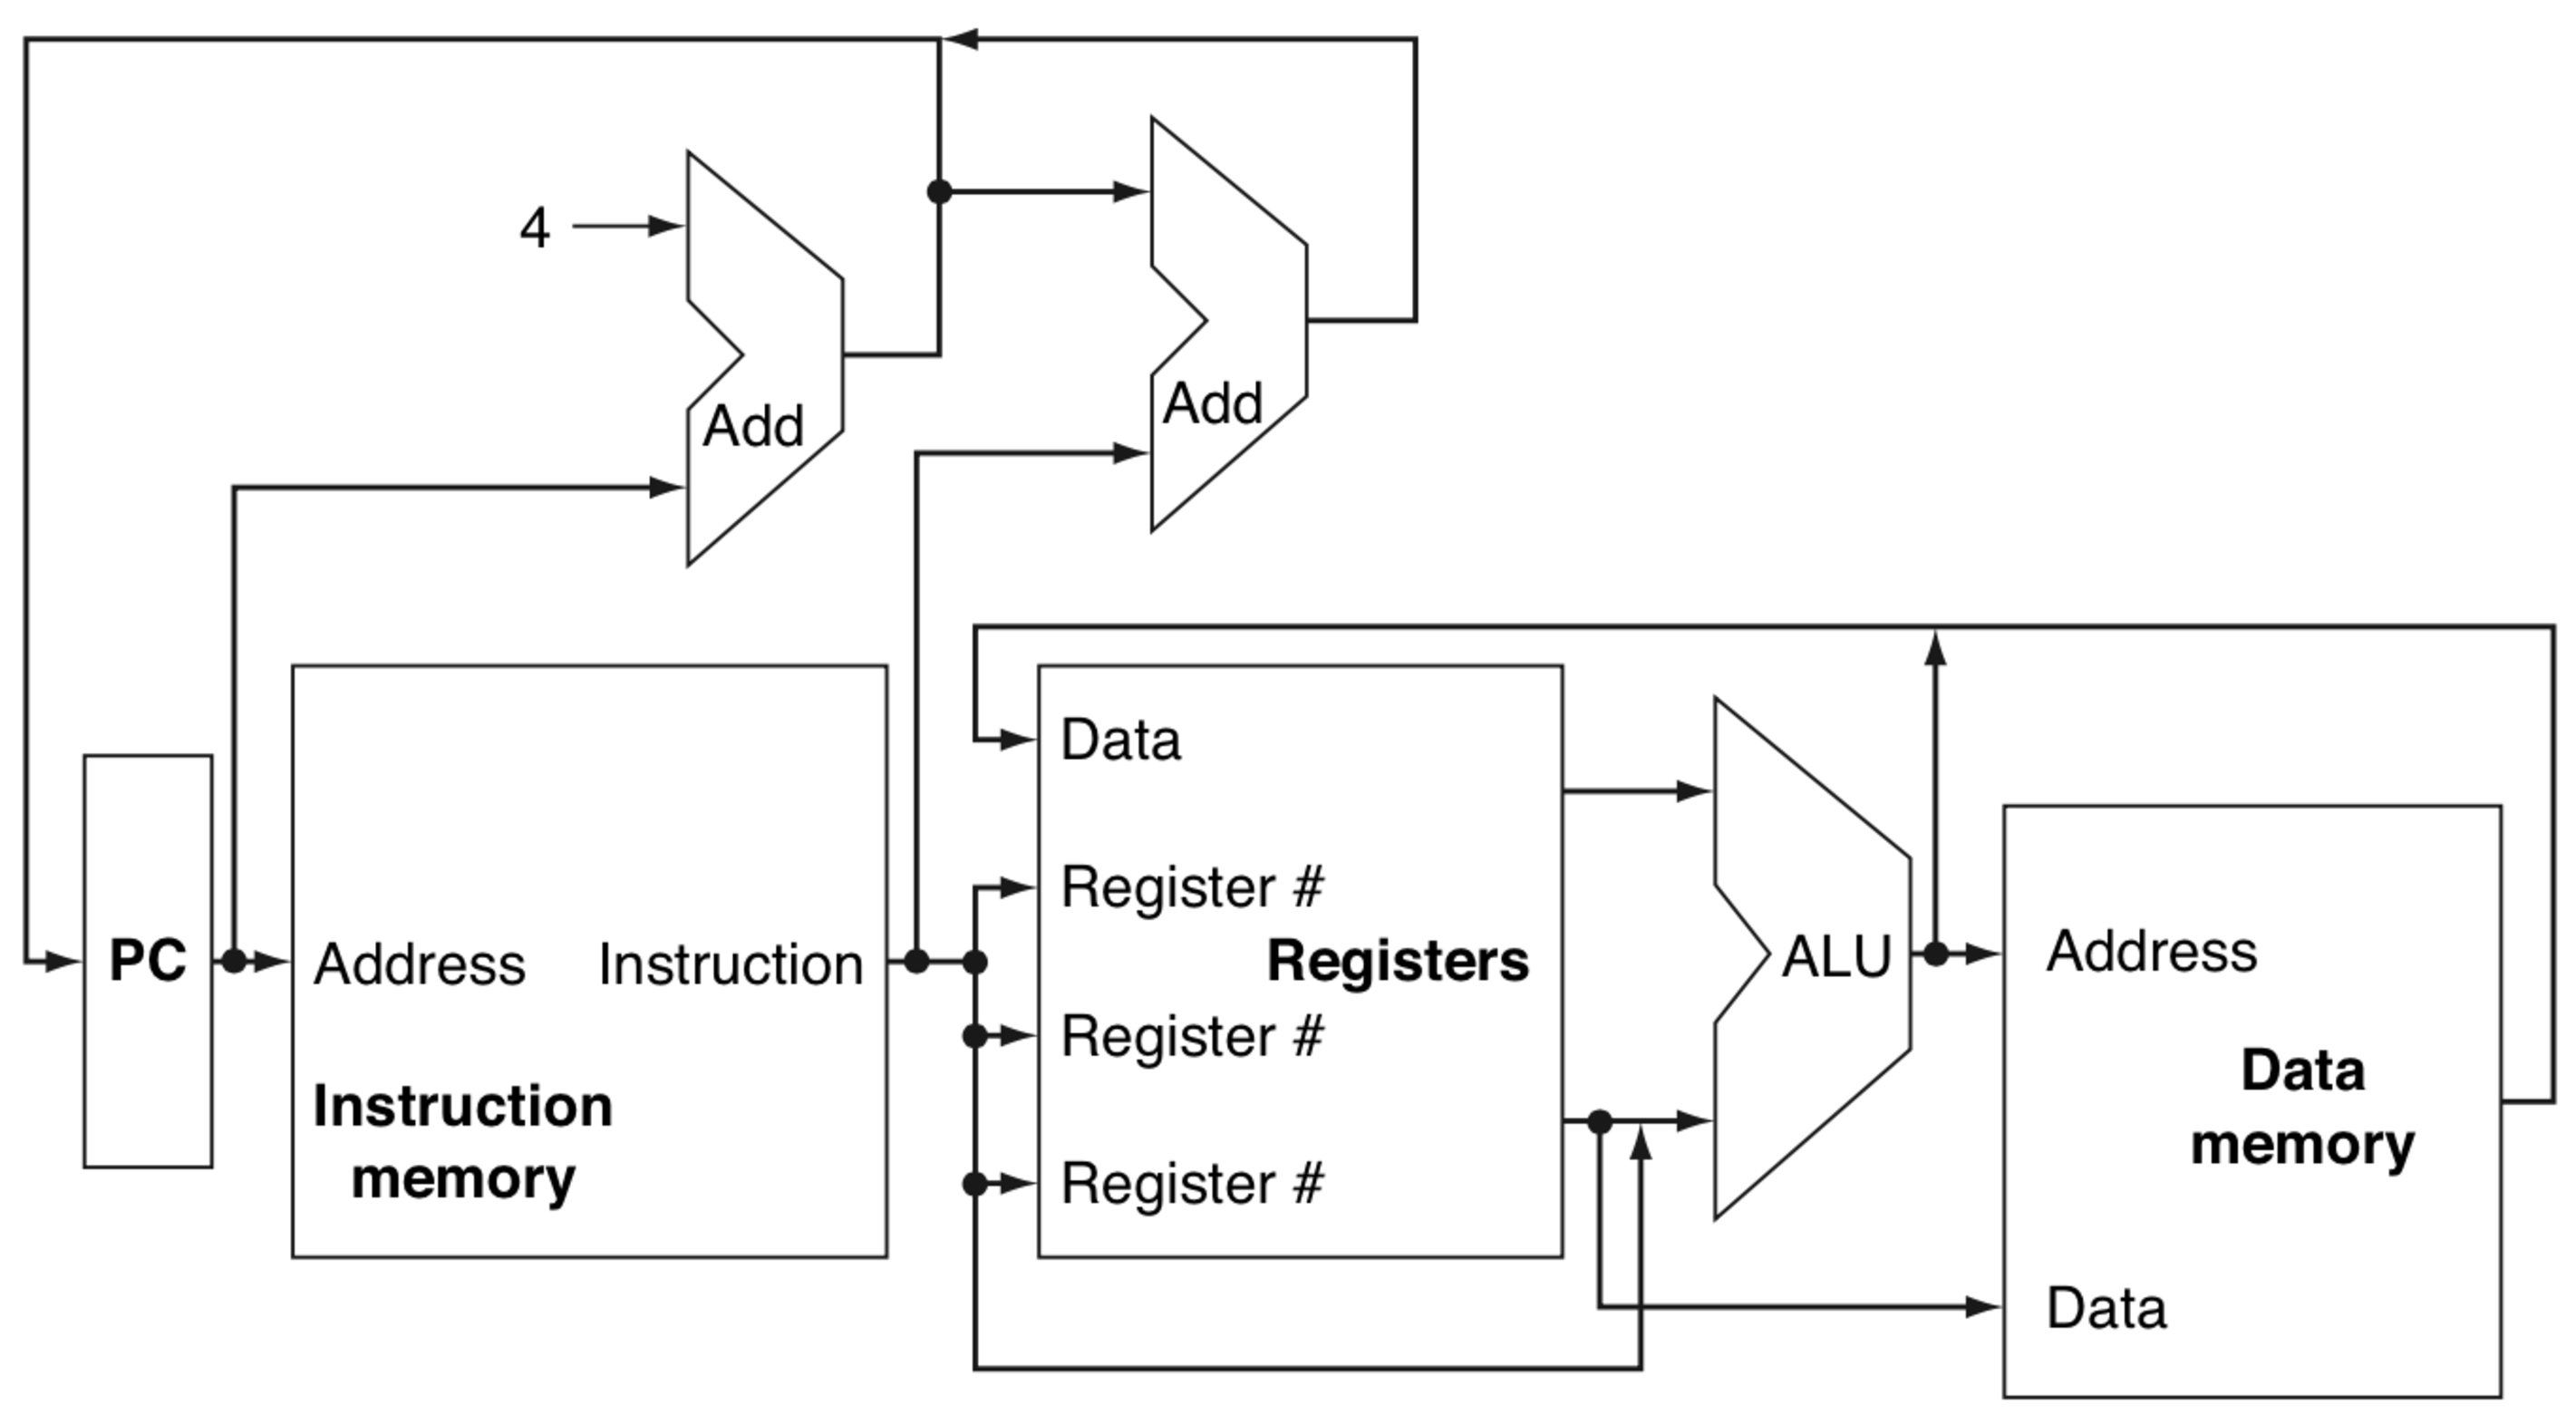
\includegraphics[width=6in]{./pics/mips-datapath}
\caption{An abstract (or high-level) view of a {\it MIPS} processor's datapath \cite{Patterson2005,Patterson2009}.}
\label{fig:mipsdatapath}
\end{figure}
%	Figure 4.1, Patterson2009, 4E, page 302
%	Figure 5.1, Patterson2005, 3E, page 287


Figure \ref{fig:mipsdatapath} shows the datapath of a simple, single-cycle microarchitectural implementation of the {\it MIPS} ISA. The datapath of a microarchitecture shows the hardware components, or logic circuits, needed to perform computation of arithmetic and logical operations as well as read/write data into memory. Its main components are logic circuits that: \vspace{-0.3cm}
\begin{enumerate} \itemsep -4pt
\item Fetch an instruction from memory, and update the program counter (PC).
\item Decode the instruction, and read register(s) (from the register file, {\tt regfile}) used by that instruction. The {\tt regfile} is shown as {\tt Registers} in Figure \ref{fig:mipsdatapath}.
\item Perform computation on an arithmetic/logical operation; i.e., the arithmetic-logical unit (ALU).
\item Read data from or write data to a memory device, or memory system (including caches). Separate memory devices can be used to store data and instructions separately. In Figure \ref{fig:mipsdatapath}, instruction memory is a memory device that stores instructions and data memory is another memory device that stores data. 
\end{enumerate}

These main components for the single-cycle microarchitectural implementation of the {\it MIPS} ISA are also used in other microarchitectural implementation of the {\it MIPS} ISA, such as the multi-cycle {\it MIPS} processor, pipelined {\it MIPS} processor, and the superscalar {\it MIPS} processor. The VLSI implementation of the main datapath components are briefly described as follows. The PC can be implemented as a binary counter or linear-feedback shift register that increments a binary number (either a 32- or 64- bit number) by four each clock cycle. A simple memory device for physical memory can be implemented using a dynamic random-access memory (DRAM). Alternatively, a simple memory system can be implemented with a three-level cache system and a DRAM, where a cache in either of the three levels can be implemented as a static random-access memory (SRAM). The ALU can be implemented with arithmetic circuits, such as adders, multipliers, and dividers. The ALU also includes comparators, shifters, one/zero detectors, encoders, and decoders \cite{Weste2011}. \\

Regarding the aforementioned design principles, I will discuss how this basic datapath satisfies the design principles mentioned earlier in Section \ref{sec:SingleCycleProcessorDesign}. Firstly, regularity in the {\it MIPS} ISA is found in majority of instructions that require the ALU to perform arithmetic or logic operations. This implies that a set of datapath components and a subset of the control logic can implement most instructions in the {\it MIPS} ISA. In addition, the regularity in the design of datapath components, such as adders in the ALU and DRAM devices, results in their simplicity. This allows architects to design simpler and faster datapaths that do not need to interface with complex control logic.  Secondly, as for smaller hardware components, components of the ALU (such as adders and shifters) are optimized for performance within area constraints. Also, for memory systems that include a multi-level cache system, the first level cache is designed to be smaller that the lower-level caches and the memory device. This allows the cache to be significantly faster than lower-level caches and the memory device. Thirdly, since most of the instructions use the ALU, a significant amount of work has been done to optimize ALU designs so that computer performance can be improved \cite{Ercegovac2004,Parhami2010,Stine2004,Farhat2004}. Lastly, the design trade-offs made for this simple datapath of a single-cycle {\it MIPS} processor demonstrates a trade-off between performance and hardware cost.




%%%%%%%%%%%%%%%%%%%%%%%%%%%%%%%%%%%%%%%%%%%
\subsection{Control Path Design for Single-Cycle Processors}
\label{ssec:ControlPathDesignforSingleCycleProcessors}

\begin{figure}[h]
\centering 
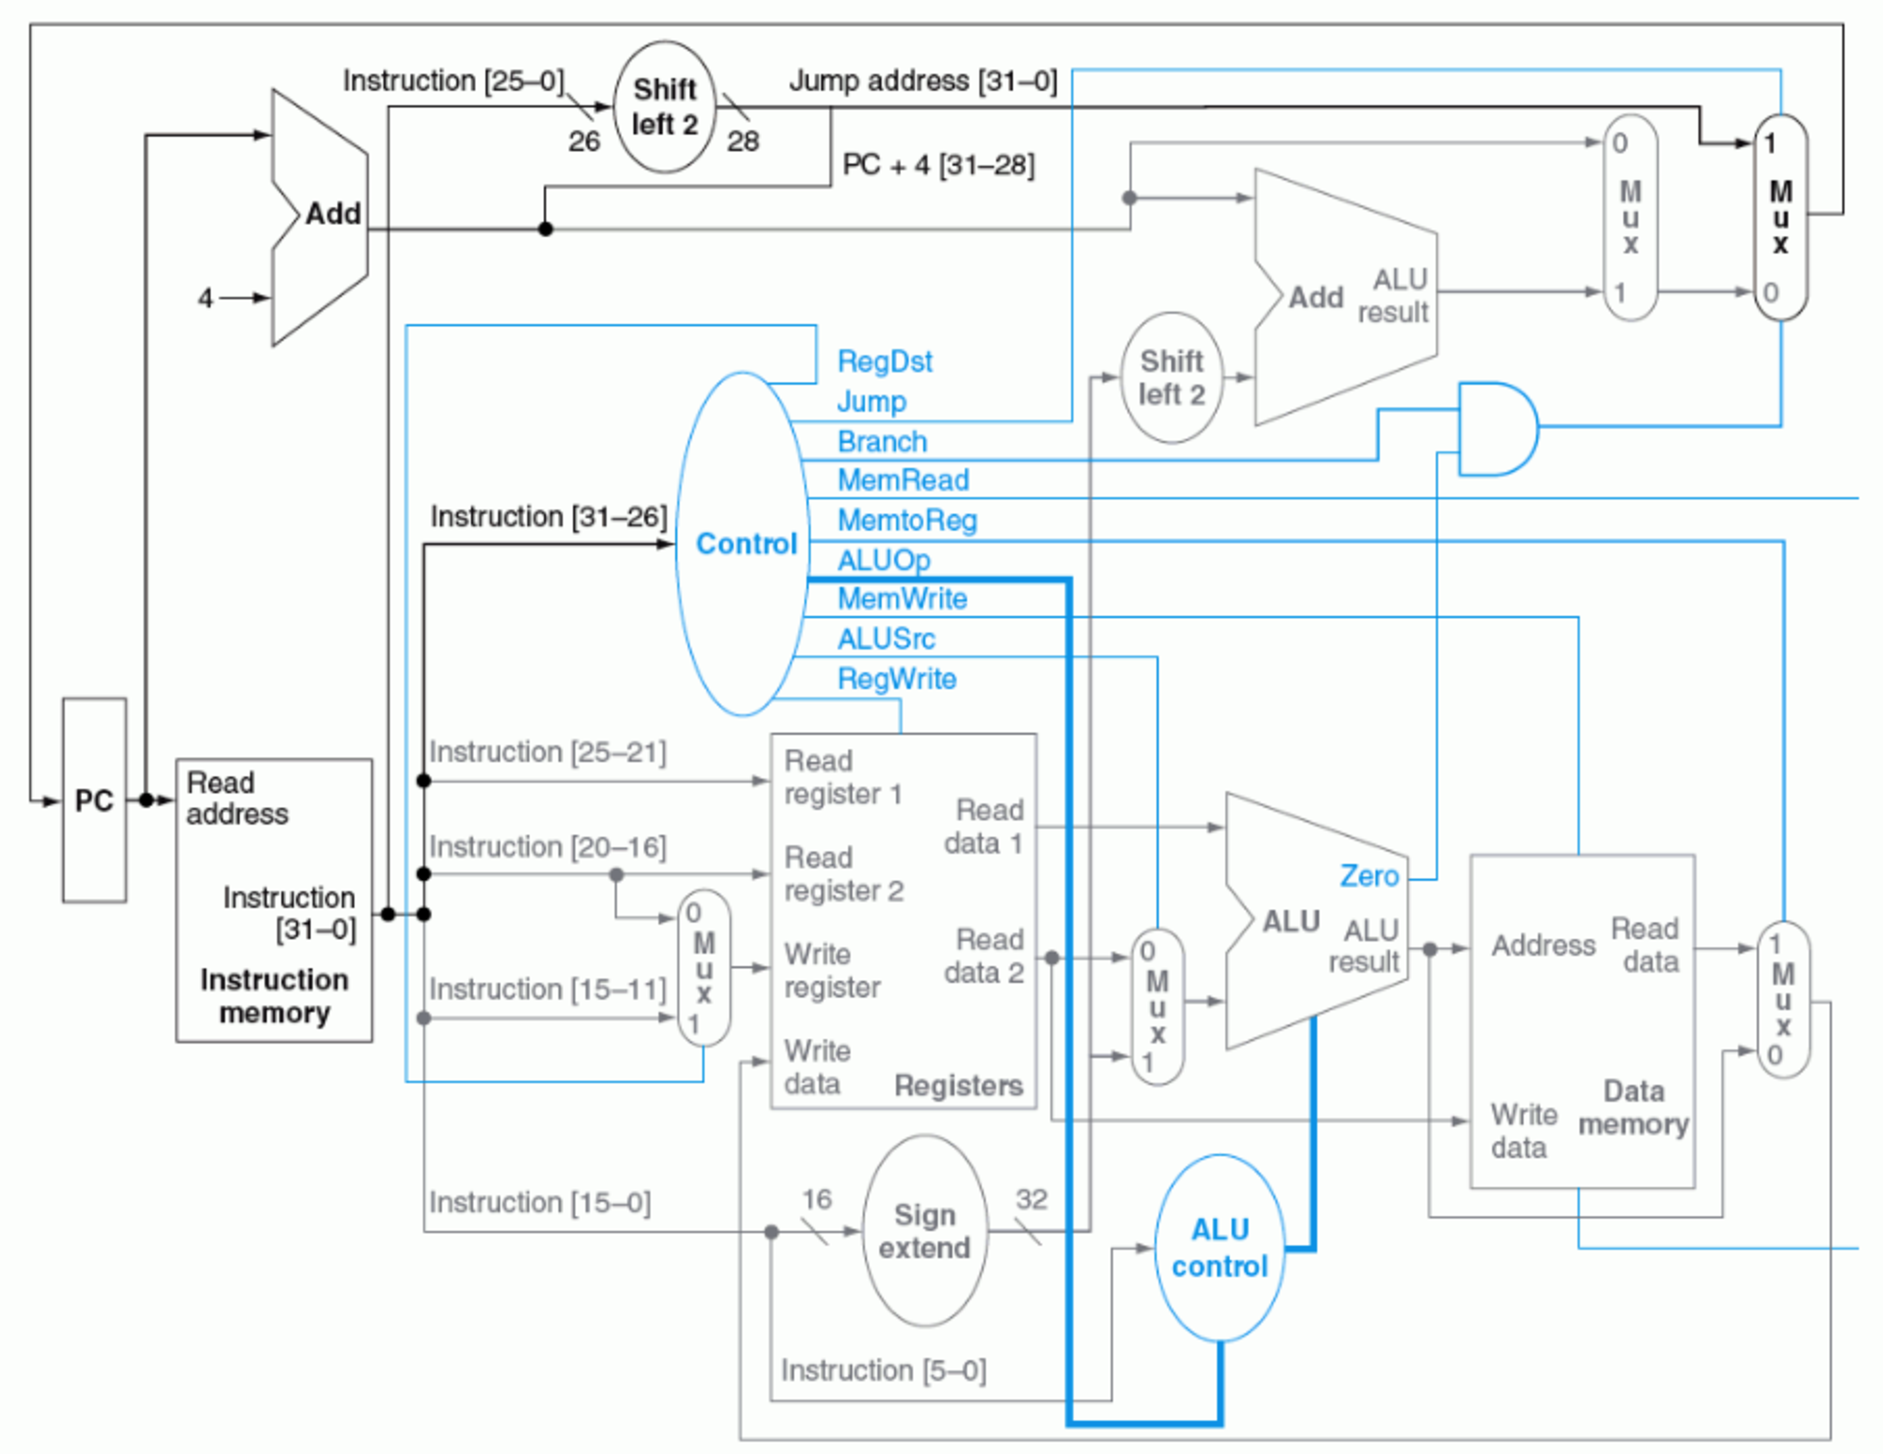
\includegraphics[width=5in]{./pics/single-cycle-processor}
\caption{Control path of a single-cycle {\it MIPS} processor, which is superimposed on the datapath of the {\it MIPS} processor \cite{Patterson2005,Patterson2009}.}
\label{fig:singlecycleprocessor}
\end{figure}
%	Figure 4.24, Patterson2009, 4E, page 329
%	Figure 5.24, Patterson2005, 3E, page 314

The control path of a processor includes a control unit to generate control signals for the processor, and wires to transmit those control signals from the control unit to various datapath components of the processor. This control unit for a single-cycle {\it MIPS} processor does not have multiple sequential states. Hence, the control unit can be implemented as a combinational logic circuit \cite{Patterson2005a}. \\

To implement the control unit as a combinational circuit, map the inputs of the control unit to its outputs. The mapping for a set of input signals to an output signal is a boolean function. This mapping can be represented as a truth table \cite{Patterson2005a} or a data structure that is typically used to represent a boolean function. Examples of such data structures include binary decision diagrams (BDDs)\cite{Hachtel1996,Hassoun2002} and AND-Inverter graphs (AIGs) \cite{Wang2009,BLSVG2011}. Electronic design automation (EDA) software can be used to optimize the size of truth tables, BDDs, or AIGs \cite{Wang2009}. By using EDA software to design and optimize the combinational circuit for the control unit, the process of designing the control path can be sped up by automation created by EDA software; also, EDA software can be used to automatically verify the correctness of the resultant circuits \cite{Scheffer2006,Scheffer2006a}. EDA software maps truth tables, BDDs, or AIGs to combinational circuits for the control unit. The combinational circuit for the control unit can be implemented as VLSI circuits using standard cells \cite{Kang2003a,Rabaey2003,Weste2011} or a programmable logic array (PLA) \cite{Patterson2005a}. \\

%The resultant hardware for the control unit is mapped by EDA software from the truth table, BDD, or AIG to a combinational circuit, using standard cells \cite{Kang2003a,Rabaey2003,Weste2011} or a programmable logic array (PLA) \cite{Patterson2005a}.





Figure \ref{fig:singlecycleprocessor} shows the datapath and the control path (in blue). The control path includes the control unit (shown as {\tt Control}) and ALU control unit {\tt ALU control}. The wiring of the buses and wires for the control path are colored in blue. The {\it PC} provides PC update, and the {\tt Instruction memory} fetches instructions from the memory device for instructions. The {\tt Registers regfile} allows data in registers to be read from the {\tt regfile}, and the lower {\tt ALU} provides computation of arithmetic and logical operations. The data memory allows data to be read from or written to memory \cite{Patterson2005,Patterson2009}. To summarize, sequentially ordered instructions from a software application would be loaded from memory into the processor for execution. After these instructions are executed, the resultant output data from executing those instructions would update the state of the processor. Next, data updated by the processor would be written to memory locations, or data would be read from memory. Finally, registers in the {\tt regfile} may have their data updated.



%%%%%%%%%%%%%%%%%%%%%%%%%%%%%%%%%%%%%%%%%%%
\subsection{Advantages and Disadvantages of Single-Cycle Processor Design}
\label{ssec:AdvantagesandDisadvantagesofSingleCycleProcessorDesign}

The single-cycle {\it MIPS} processor has the advantage of a simple datapath, which can be easily designed and verified. However, its major disadvantage is that it is computationally inefficient, since it requires all instructions to be executed in one clock cycle. Therefore, the CPI for the single-cycle {\it MIPS} processor is one. Since the latency of memory access instructions tends to be much slower than the latency of other instructions, the speed of the single-cycle {\it MIPS} processor is limited to the memory access speed \cite{Patterson2005,Patterson2009}.















































%%%%%%%%%%%%%%%%%%%%%%%%%%%%%%%%%%%%%%%%%
%	Multi-cycle Processor Design
%	This is written by Zhiyang Ong as a template for writing reports.

%	The MIT License (MIT)

%	Copyright (c) <2014> <Zhiyang Ong>

%	Permission is hereby granted, free of charge, to any person obtaining a copy of this software and associated documentation files (the "Software"), to deal in the Software without restriction, including without limitation the rights to use, copy, modify, merge, publish, distribute, sublicense, and/or sell copies of the Software, and to permit persons to whom the Software is furnished to do so, subject to the following conditions:

%	The above copyright notice and this permission notice shall be included in all copies or substantial portions of the Software.

%	THE SOFTWARE IS PROVIDED "AS IS", WITHOUT WARRANTY OF ANY KIND, EXPRESS OR IMPLIED, INCLUDING BUT NOT LIMITED TO THE WARRANTIES OF MERCHANTABILITY, FITNESS FOR A PARTICULAR PURPOSE AND NONINFRINGEMENT. IN NO EVENT SHALL THE AUTHORS OR COPYRIGHT HOLDERS BE LIABLE FOR ANY CLAIM, DAMAGES OR OTHER LIABILITY, WHETHER IN AN ACTION OF CONTRACT, TORT OR OTHERWISE, ARISING FROM, OUT OF OR IN CONNECTION WITH THE SOFTWARE OR THE USE OR OTHER DEALINGS IN THE SOFTWARE.

%	Email address: echo "cukj -wb- 23wU4X5M589 TROJANS cqkH wiuz2y 0f Mw Stanford" | awk '{ sub("23wU4X5M589","F.d_c_b. ") sub("Stanford","d0mA1n"); print $5, $2, $8; for (i=1; i<=1; i++) print "6\b"; print $9, $7, $6 }' | sed y/kqcbuHwM62z/gnotrzadqmC/ | tr 'q' ' ' | tr -d [:cntrl:] | tr -d 'ir' | tr y "\n"

%%%%%%%%%%%%%%%%%%%%%%%%%%%%%%%%%%%%%%%%%%%%%%


%%%%%%%%%%%%%%%%%%%%%%%%%%%%%%%%%%%%%%%%%%%
\section{Multi-Cycle Processor Design}
\label{sec:MultiCycleProcessorDesign}


%	Figure 5.39 and 5.40 from \cite{Patterson2005}
To improve the performance of the single-cycle {\it MIPS} processor (see \S\ref{sec:SingleCycleProcessorDesign}), a better semiconductor manufacturing process technology can be used to manufacture implementations of the microarchitecture as a VLSI system. Alternatively, the microarchitecture can be modified to significantly improve the performance of the processor. For each instruction in the {\it MIPS} ISA, decompose the instruction into steps based on the functional units required to complete executing that instruction. That is, if an instruction needs five components, it shall be decomposed/partitioned into five steps. Each step of the decomposed instruction shall take one clock cycle. In general, the datapath in Subsection \ref{ssec:DatapathDesignforSingleCycleProcessors} (see Figure \ref{fig:mipsdatapath}) can be decomposed into the following five stages \cite{Patterson2005}: \vspace{-0.3cm}
\begin{enumerate} \itemsep -4pt
\item Instruction fetch (IF). Instructions are fetched from memory and the program counter (PC) is updated.
\item Instruction decode (ID). Instructions are decoded and register(s) are read from the register file {\tt regfile}.
\item Execution (EX). Arithmetic/logical operations are performed by the arithmetic-logical unit (ALU).
\item Memory access (MEM). Read data from or write data to the memory device or memory system (including caches).
\item Write-back (WB). Complete memory read operations (i.e., load operations).
\end{enumerate}

Each of the stages listed above can be a step for a decomposed instruction. Since different instructions require different number of stages, the CPI for instructions in the {\it MIPS} ISA would vary for microarchitectures that allow instructions to complete in a range of clock cycles. These microarchitectures are known as multi-cycle processors. A multi-cycle processor allows a functional unit to be used multiple times per clock cycle. This reduces the amount of required hardware resources/components and encourages microarchitects (or processor architects) to share hardware resources between different steps of an instruction \cite{Patterson2005}. \\

The rest of this section is organized as follows. In Subsection \ref{ssec:DatapathDesignforMultiCycleProcessors}, I discuss the datapath design for the multi-cycle {\it MIPS} processor. Following this, in Subection \ref{ssec:ControlPathDesignforMultiCycleProcessors}, I describe the control path of the multi-cycle {\it MIPS} processor, including a brief discussion of how to implement the finite state machine representation of the control unit (in the control path) as a sequential circuit (see \S\ref{sssec:FiniteStateControl}). Next, I compare the advantages and disadvantages of the multi-cycle {\it MIPS} processor with the single-cycle {\it MIPS} processor (see \S\ref{sec:SingleCycleProcessorDesign}) in Subsection \ref{ssec:AdvantagesandDisadvantagesofMultiCycleProcessorDesign}. Lastly, in Subsection \ref{ssec:Microprogramming}, I discuss how microprogramming can be used to reduce the hardware complexity of a microarchitecture's control path, and reduce the amount of effort needed to design that microarchitecture as a VLSI system.



%%%%%%%%%%%%%%%%%%%%%%%%%%%%%%%%%%%%%%%%%%%
\subsection{Datapath Design for Multi-Cycle Processor}
\label{ssec:DatapathDesignforMultiCycleProcessors}

\begin{figure}[h]
\centering 
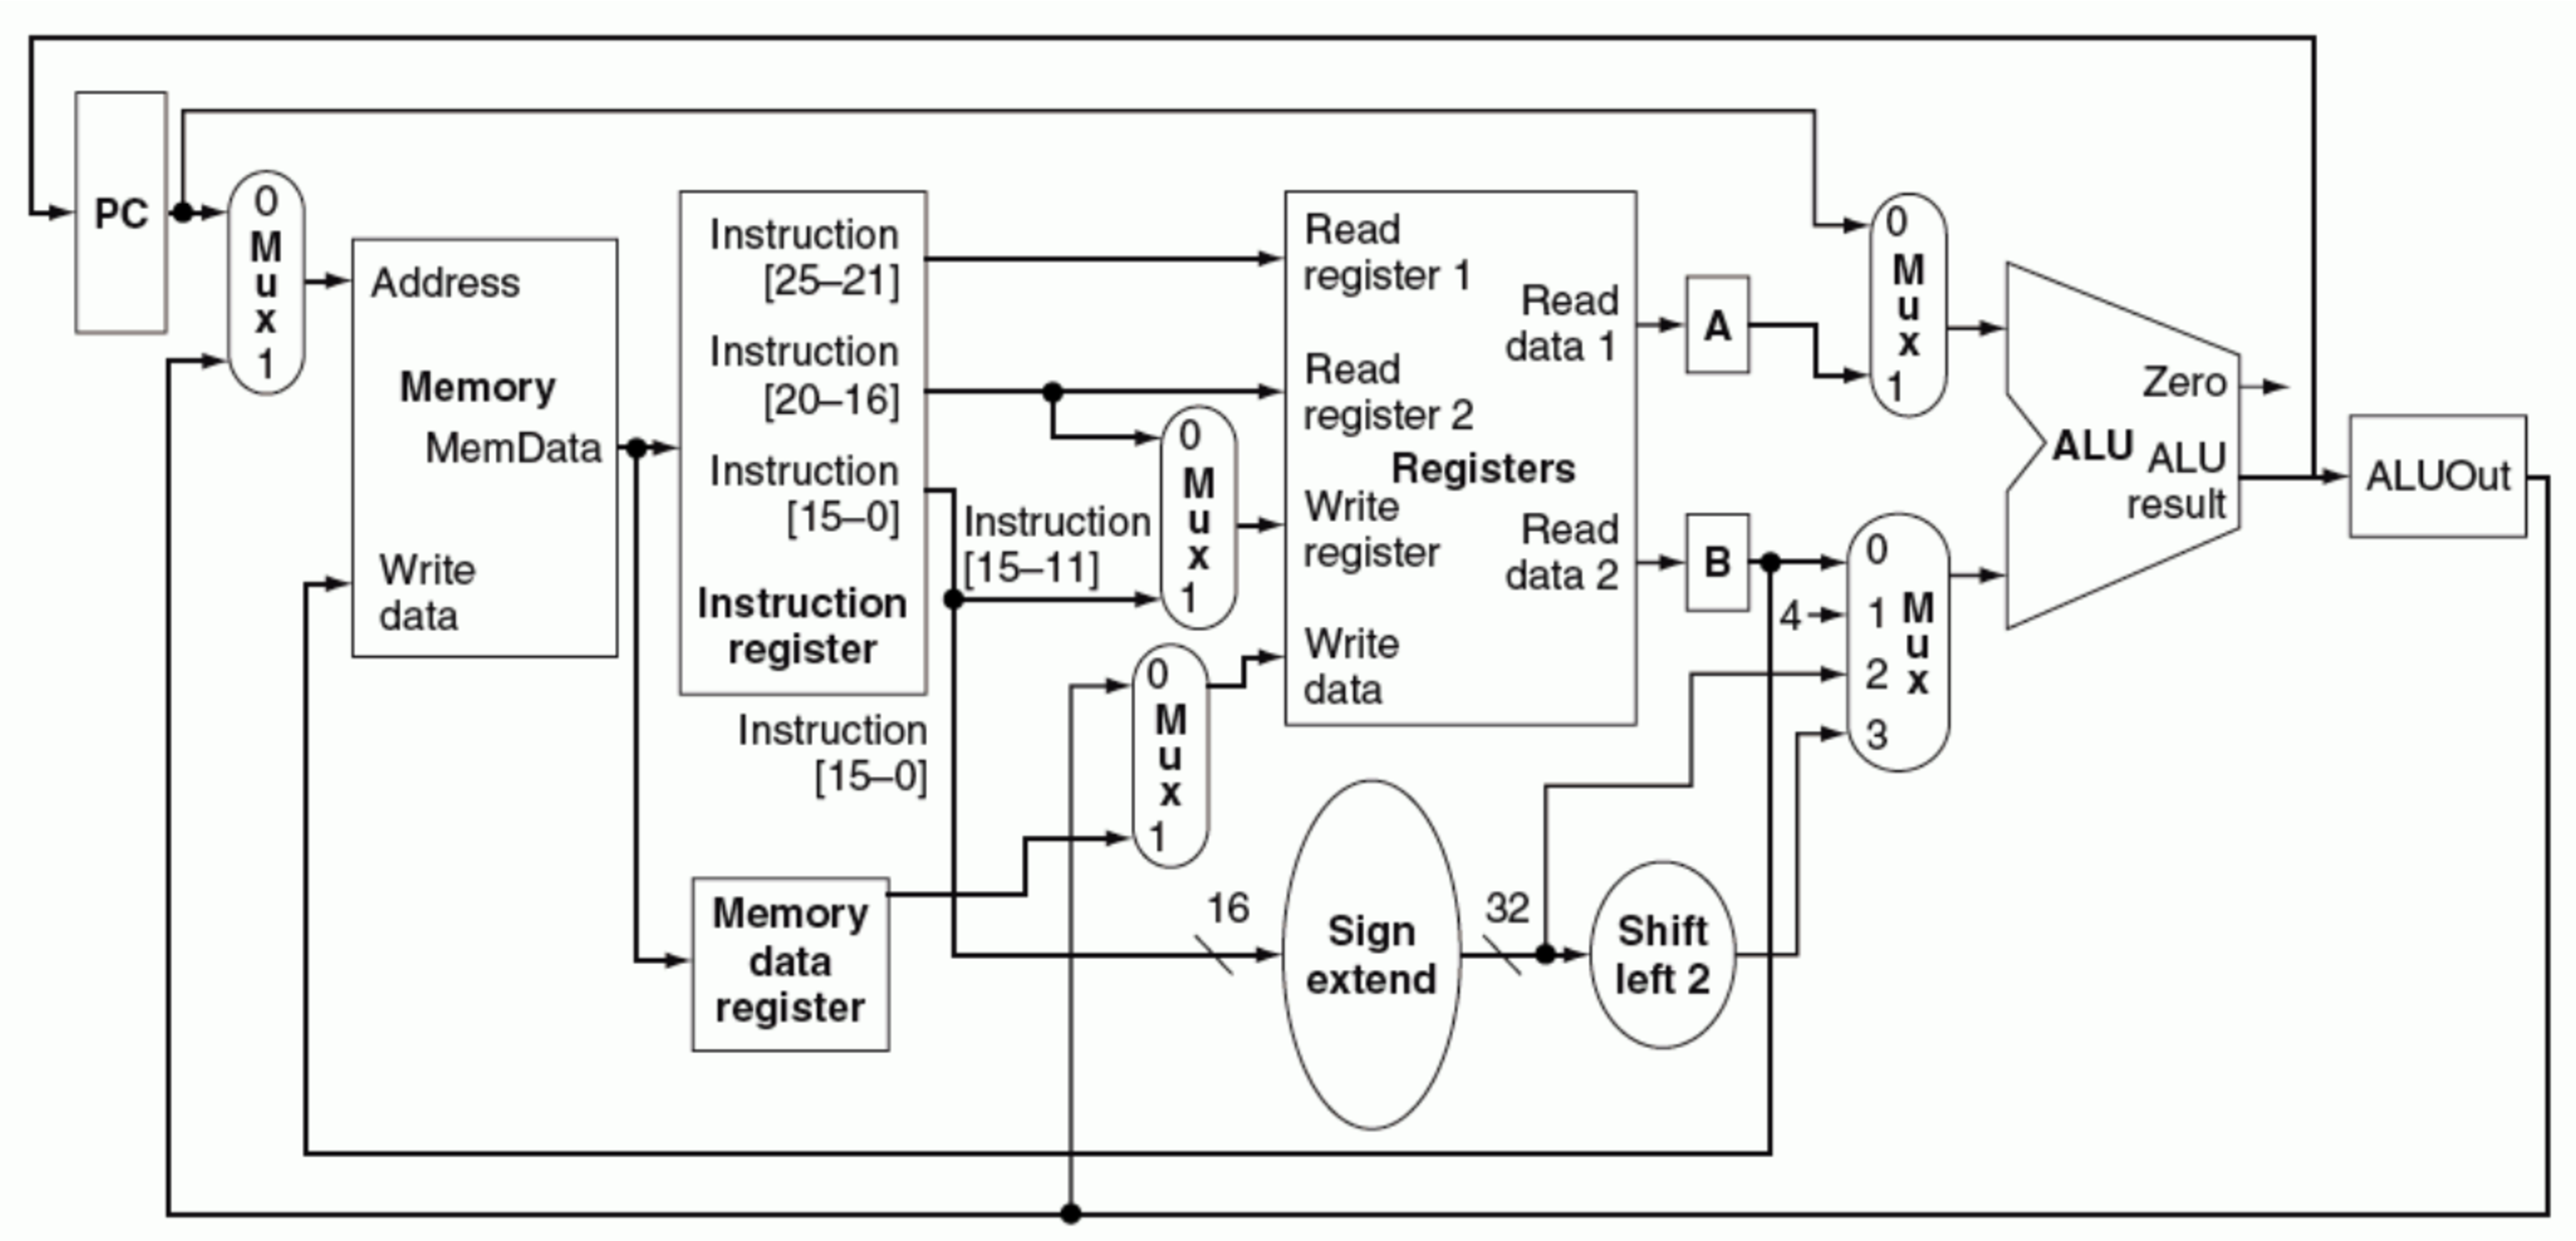
\includegraphics[width=6in]{./pics/multi-cycle-processor-data-path2}
\caption{Datapath of a multi-cycle {\it MIPS} processor \cite{Patterson2005}.}
\label{fig:multicycleprocessordatapath2}
\end{figure}
%	Figure 5.39, \cite{Patterson2005}, pp. 344


Figure \ref{fig:multicycleprocessordatapath2} shows the datapath of a multi-cycle {\it MIPS} processor \cite{Patterson2005}. The datapath design is obtained by partitioning the datapath of the single-cycle {\it MIPS} processor into hardware components needed for decomposed steps of instructions. As aforementioned, datapath components (or hardware resources in the datapath) of the single-cycle {\it MIPS} processor (see Figure \ref{fig:singlecycleprocessor}) are shared to reduce the number of components in the datapath. For example, the data and instruction memory devices are combined into a memory device for data and instructions. In addition, only one ALU is needed in the datapath, since it can be reused in different clock cycles during the execution of an instruction \cite{Patterson2005}. \\

For a given instruction, it can use data for multiple clock cycles, since an instruction would require more than two clock cycles to load and complete execution. Therefore, state elements are used to provide this data for multiple clock cycles. State elements are visible to software developers and include the following: PC counter, register file, memory device/system, and registers (for temporary storage of data that will be used in later cycles of a given instruction). The following temporary registers are added to the microarchitecture of the multi-cycle {\it MIPS} processor \cite{Patterson2005}: \vspace{-0.3cm}
\begin{enumerate} \itemsep -4pt
\item Instruction register (IR). IR is used to save the output of an instruction read operation for use in the same clock cycle.
\item Memory data register (MDR). MDR is used to save the output of an data read operation for use in the same clock cycle.
\item Registers {\tt A} and {\tt B}. They are used to hold the values of register operands of an instruction and serve as a buffer between the register file and the ALU.
\item Register {\tt ALUOut}. It holds the output of the ALU.
\end{enumerate}

Therefore, for the multi-cycle {\it MIPS} processor to function correctly, the clock cycle has to be determined by the longest latency of the aforementioned five stages. In turn, this determines the performance of the multi-cycle {\it MIPS} processor.


%%%%%%%%%%%%%%%%%%%%%%%%%%%%%%%%%%%%%%%%%%%
\subsection{Control Path Design for Multi-Cycle Processor}
\label{ssec:ControlPathDesignforMultiCycleProcessors}

\begin{figure}[h]
\centering 
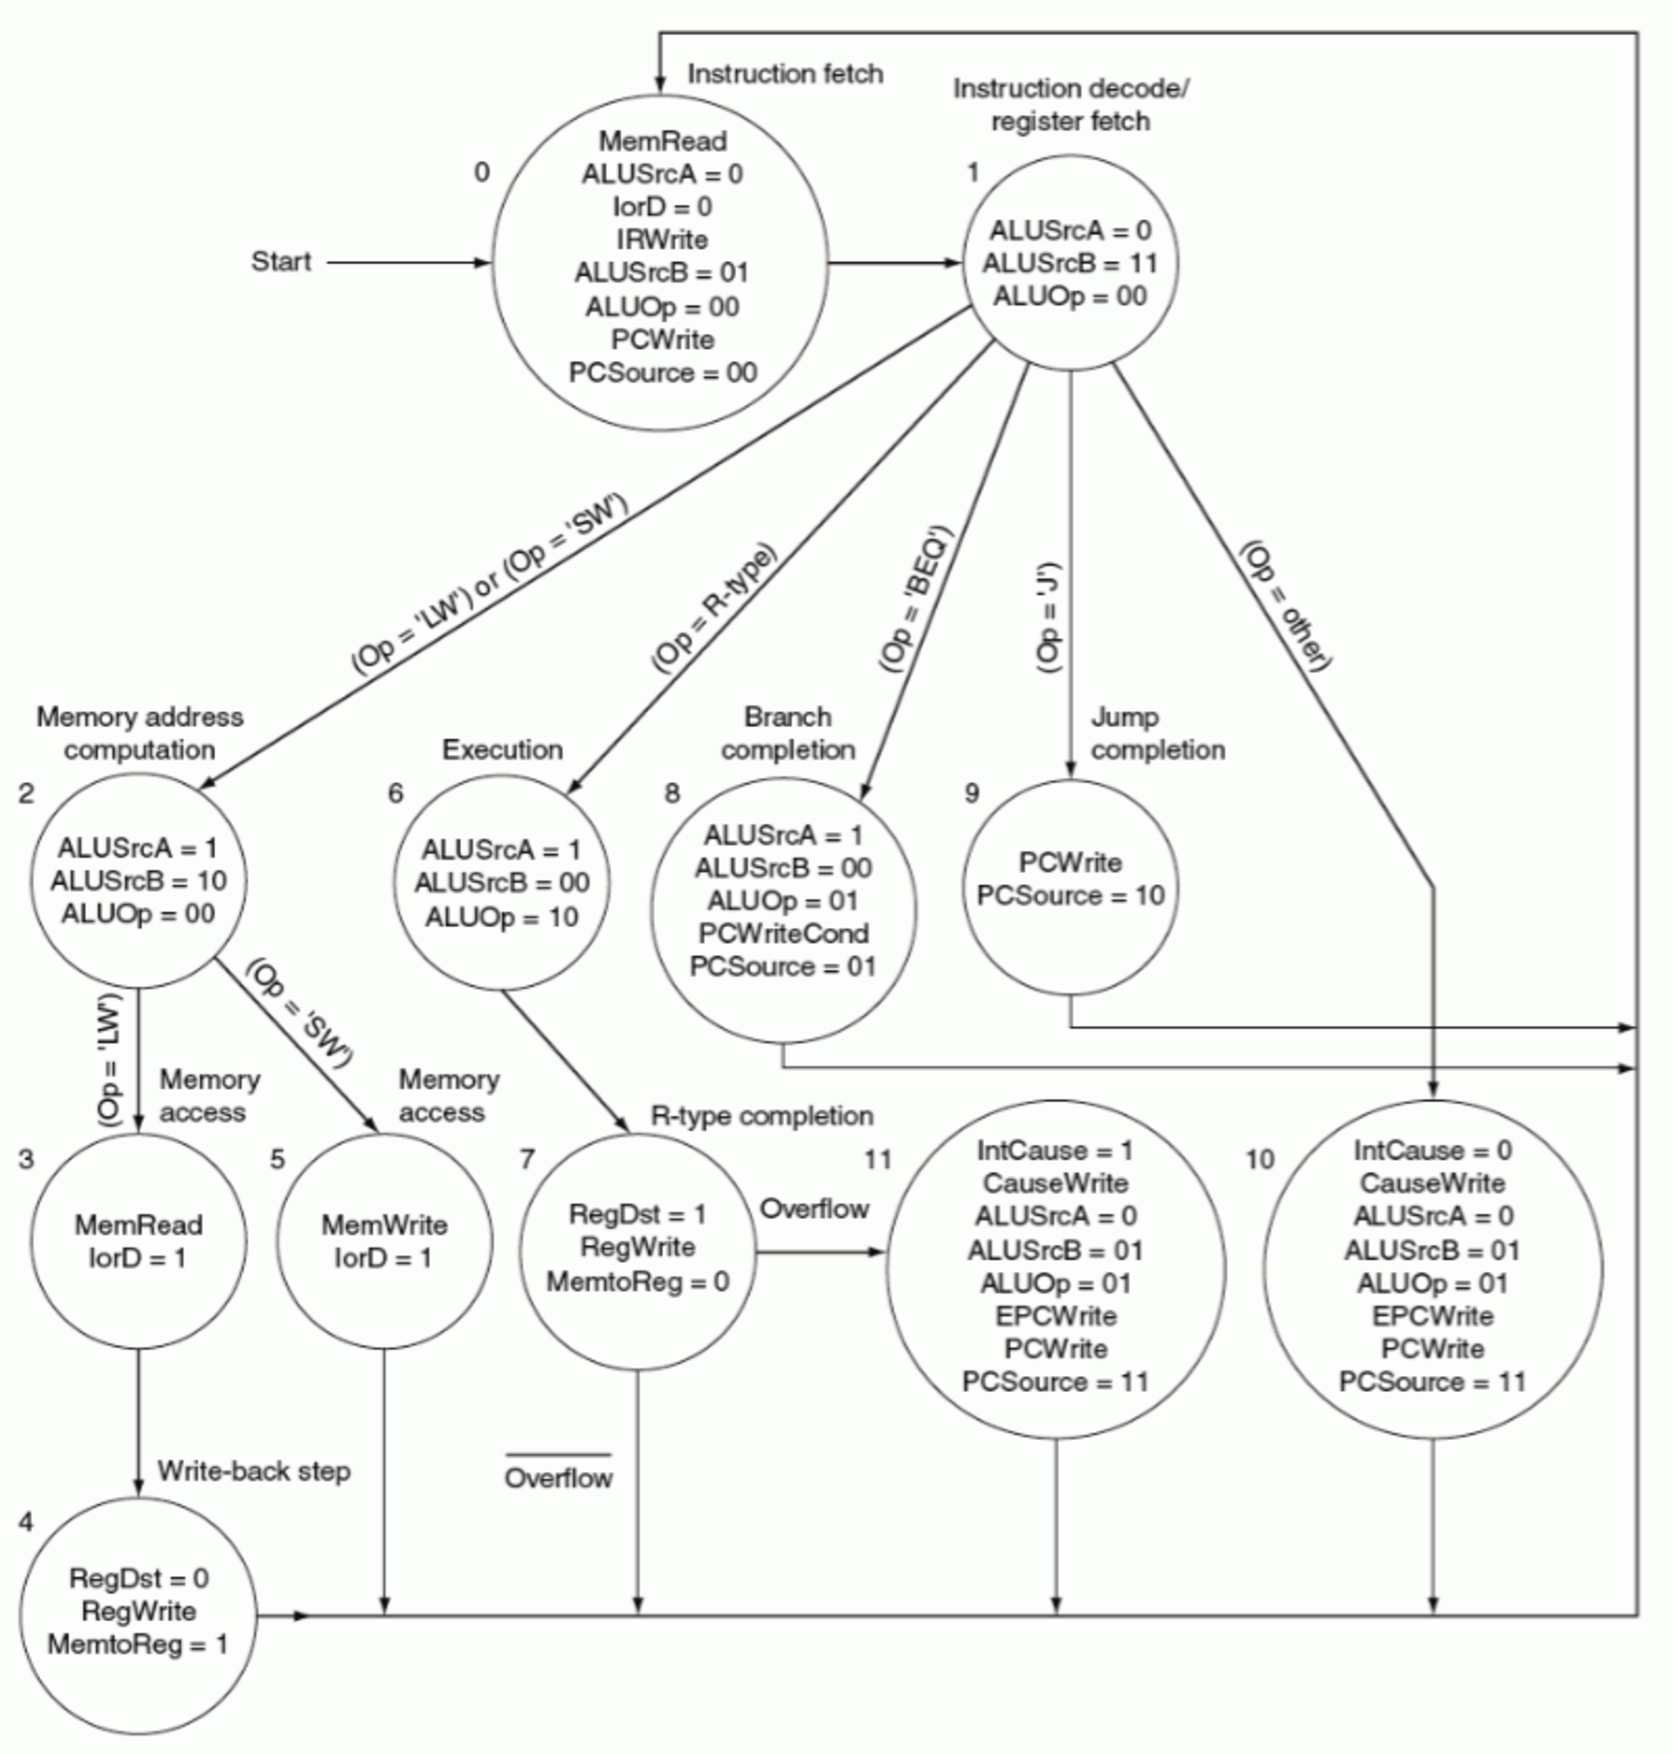
\includegraphics[width=6in]{./pics/multi-cycle-processor-fsm-ctrl-logic}
\caption{Finite state machine representation of the control unit for a multi-cycle {\it MIPS} processor \cite{Patterson2005,Patterson2005a}.}
\label{fig:multicycleprocessorfsmctrllogic}
\end{figure}
%	Figure 5.40, \cite{Patterson2005}, pp. 345

The control unit for a multi-cycle {\it MIPS} processor has multiple sequential states. Therefore, this control unit needs to be implemented as a sequential logic circuit. The sequential behavior of a sequential logic/digital circuit can be represented as a finite state machine (FSM) \cite{Patterson2005a}. Subsection \ref{sssec:FiniteStateControl} provides a description of transforming a FSM representation of the control unit into a sequential digital circuit. Alternatively, microprograms can be used to implement the control path of the processor and simplify the microarchitecture design of the multi-cycle processor (see \S\ref{ssec:Microprogramming}) \cite{Patterson2005}. \\


\begin{figure}[h]
\centering 
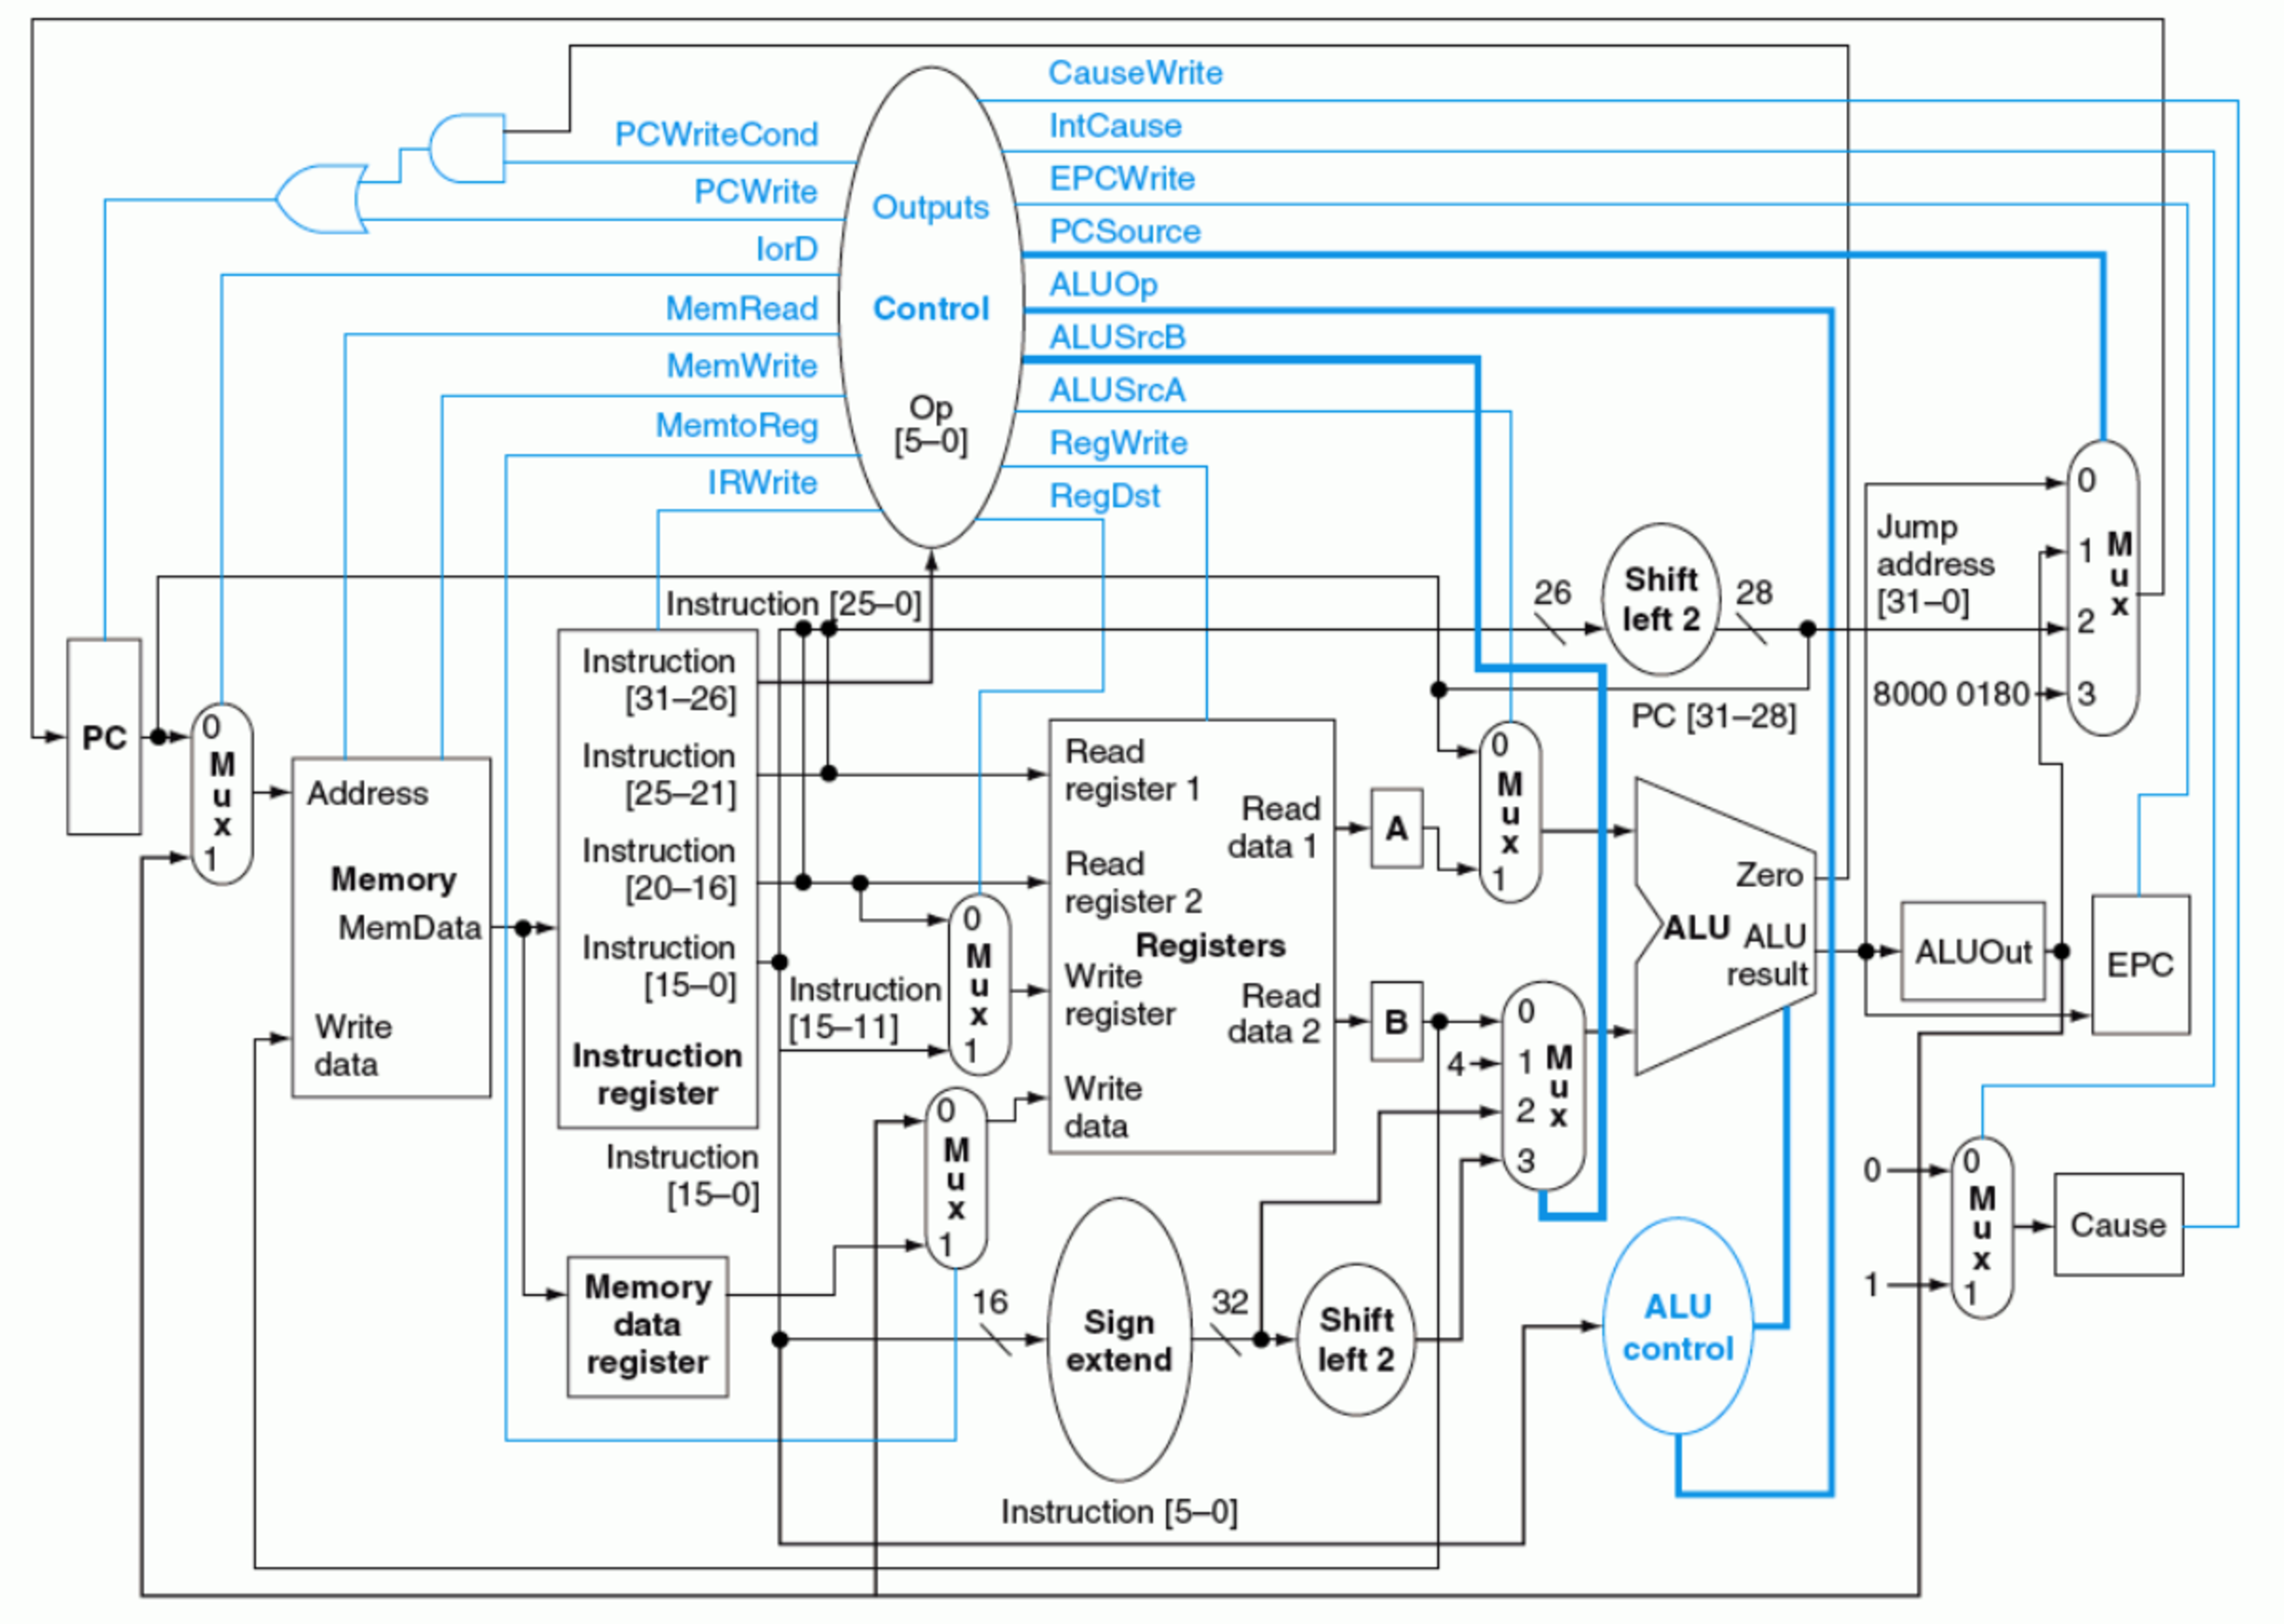
\includegraphics[width=6in]{./pics/multi-cycle-processor}
\caption{Microarchitecture for a multi-cycle {\it MIPS} processor \cite{Patterson2005}.}
\label{fig:multicycleprocessor}
\end{figure}



Figure \ref{fig:multicycleprocessorfsmctrllogic} shows the FSM for a multi-cycle {\it MIPS} processor \cite{Patterson2005,Patterson2005a}. It indicates the states that the processor can be in and how a state can transit to another state. The next state function determines the transition from the current state to the next state. The stages IF, ID, and WB are each represented as a stage in the FSM. Instructions that require the use of the ALU are categorized into memory access operations, execution, branch completion, and jump completion. Each category is represented as a state in the FSM. Similarly, the memory access operations for {\tt read} and {\tt write} are each represented as a state \cite{Patterson2005}. Subsection \ref{sssec:FiniteStateControl} briefly describes how this FSM can be mapped into a sequential circuit. \\

Figure \ref{fig:multicycleprocessor} shows the microarchitecture of the multi-cycle processor that includes the control path (colored in blue) and the datapath \cite{Patterson2005}. It integrates the datapath (see Figure \ref{fig:multicycleprocessordatapath2}) in Subsection \ref{ssec:DatapathDesignforMultiCycleProcessors} with the control logic (see Figure \ref{fig:controllogicmulticycleprocessor} in \S\ref{sssec:FiniteStateControl}) and associated wiring. It also has addition control logic for detecting and handling exceptions.








%%%%%%%%%%%%%%%%%%%%%%%%%%%%%%%%%%%%%%%%%%%
\subsubsection{Finite State Control}
\label{sssec:FiniteStateControl}

The process of implementing a FSM as a sequential circuit is described briefly as follows. \\

Firstly, label each state in the FSM as a binary number, which would be stored in a state register in the sequential circuit \cite{Patterson2005a}; a state register is a flip-flop circuit \cite{Kang2003a,Rabaey2003,Weste2011}. Next, represent each state and output signal in the FSM as a boolean variable. Determine a boolean function of states to obtain the boolean value for each output signal in the FSM. The combinational circuit derived from this boolean function is the output logic circuit for the FSM. Subsequently, design the combinational circuit needed to determine the next state for a given state in the FSM. That is, for each possible next state in the FSM, represent that state as a boolean variable. The value of the boolean variable is determined by a boolean function of the states and output signals of the FSM. Here, each state or output signal is represented as a boolean variable. The second boolean function is mapped to a combinational circuit. This combinational circuit is called the next state logic circuit for the FSM. \\


\begin{figure}[h]
\centering 
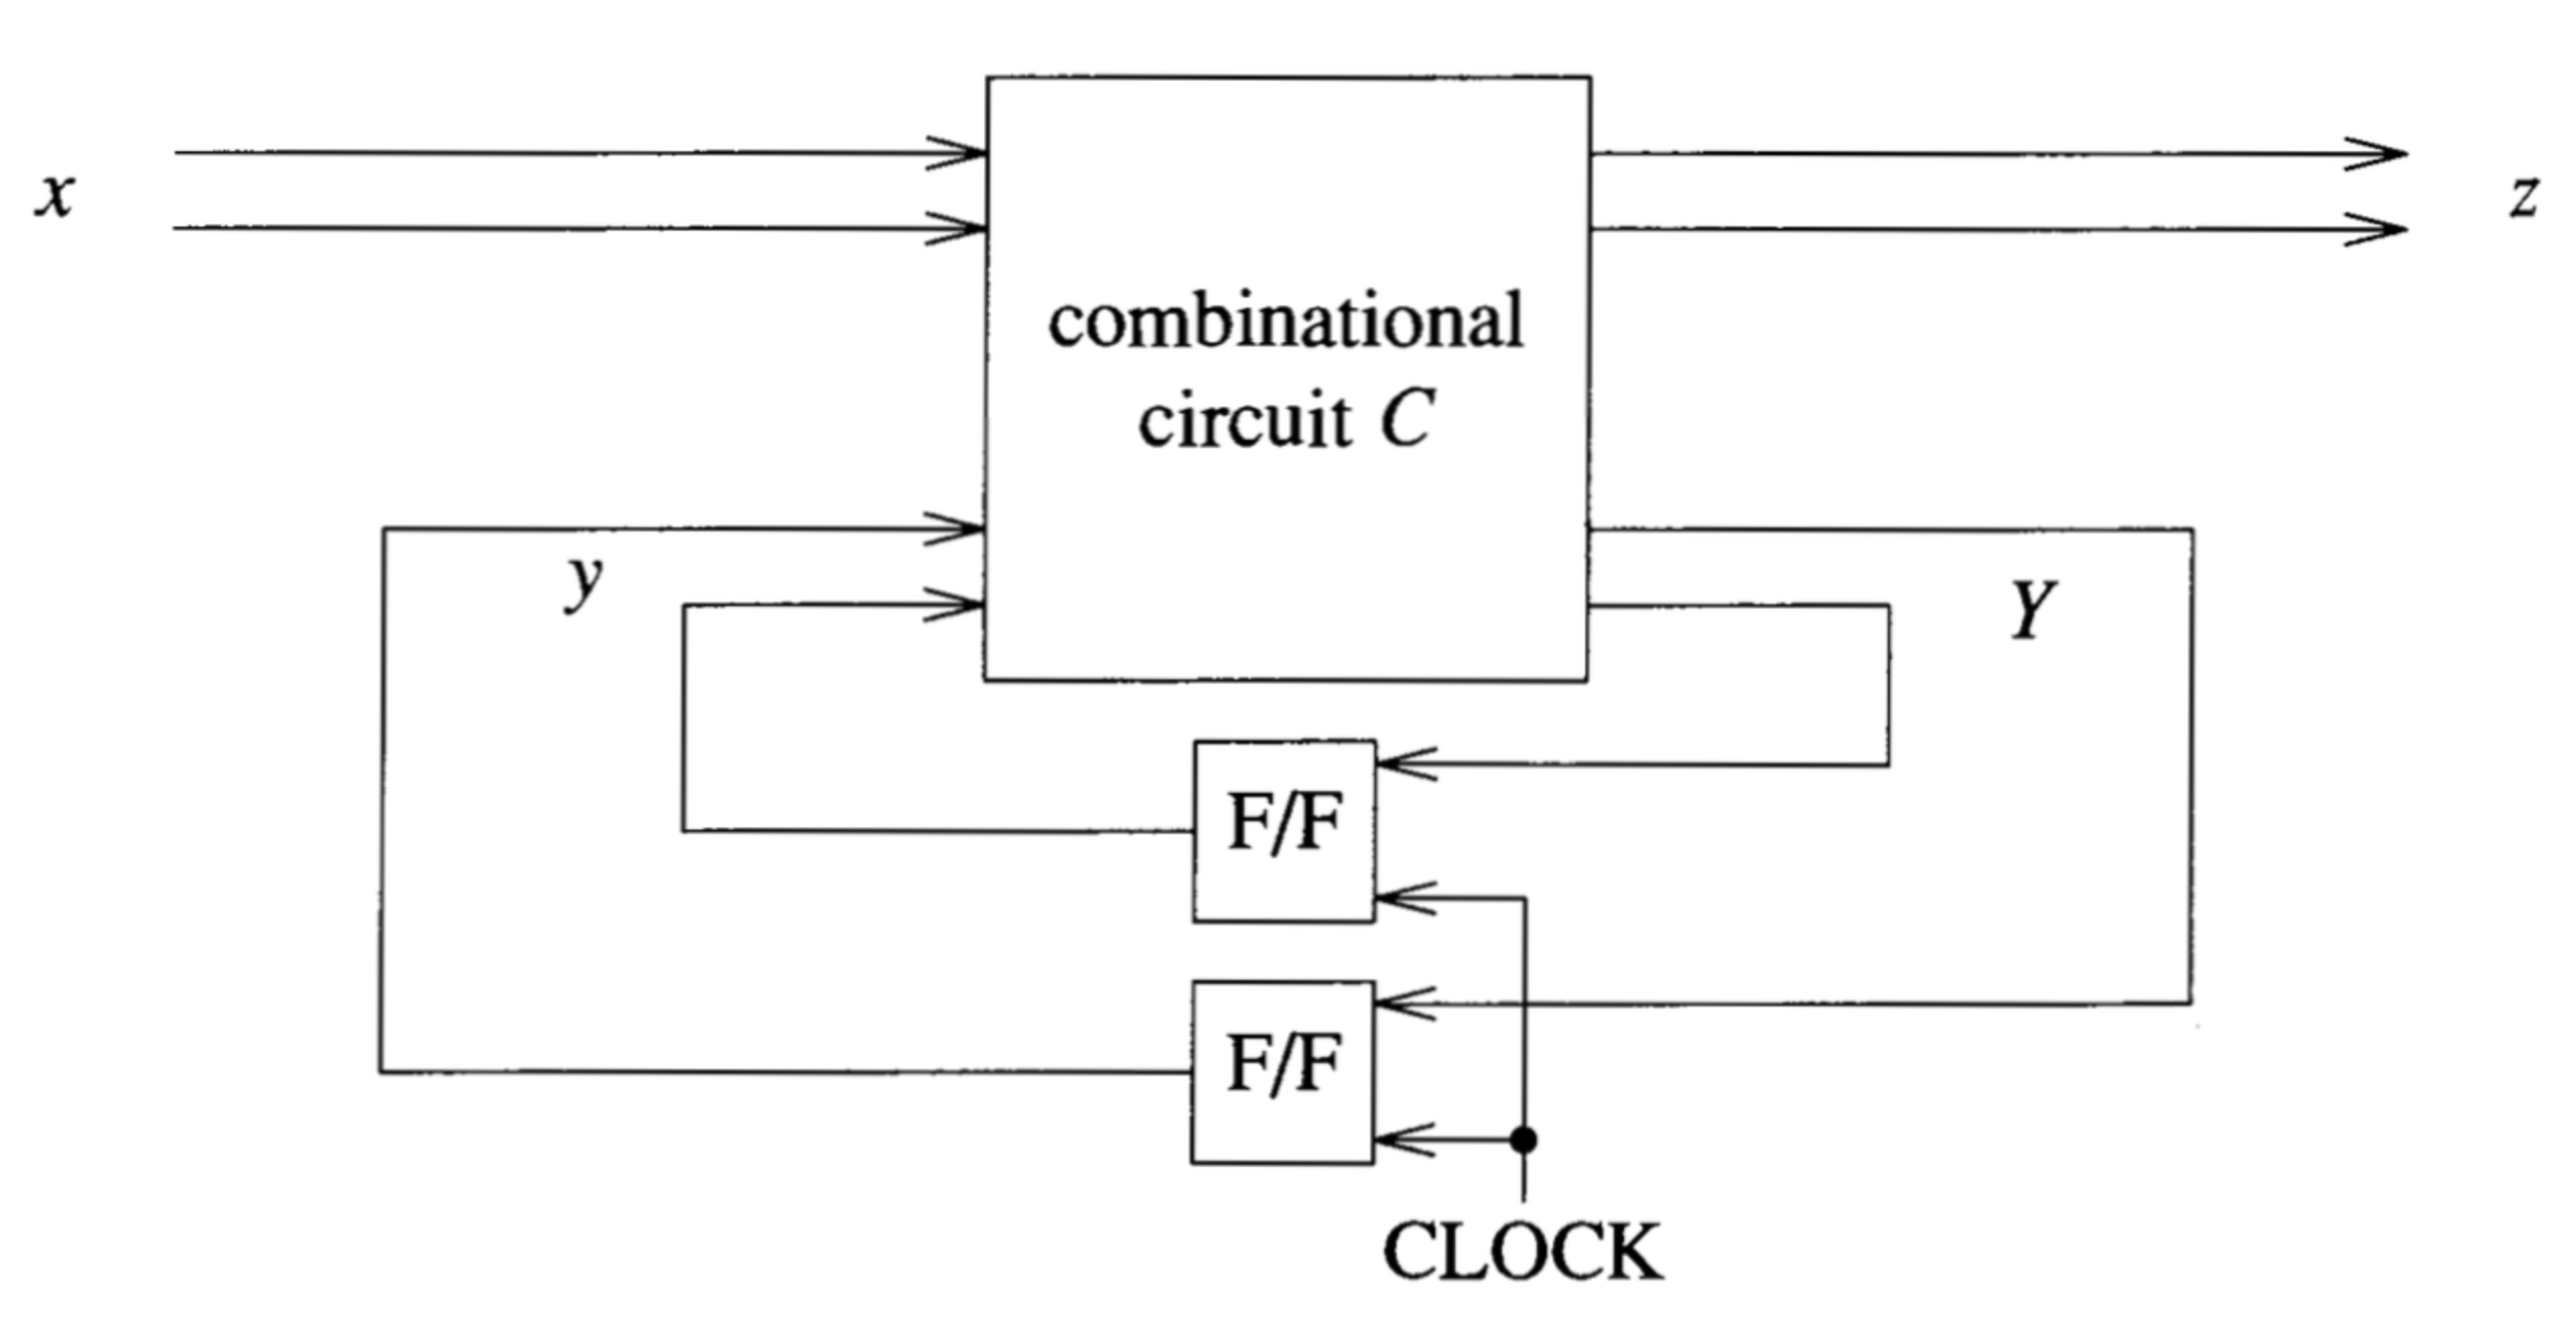
\includegraphics[width=4in]{./pics/canonical-sequential-logic-circuit}
\caption{A schematic for the canonical circuit topology for a synchronous sequential circuit. The clock signal {\tt CLOCK} provides synchrony for the sequential circuit. The combinational circuit {\it C} represents the next state logic and output logic circuits of the sequential circuit's finite state machine (FSM) representation, and the pair of flip-flops (F/F) provide the state storage for the FSM \cite{Abramovici1990}.}
\label{fig:canonicalsequentiallogiccircuit}
\end{figure}
%	Figure 2.5, pp. 14, \cite{Abramovici1990}

Figure \ref{fig:canonicalsequentiallogiccircuit} shows the canonical circuit topology for a synchronous sequential circuit, which encapsulates the next state logic and the output logic circuits as the combinational circuit {\it C} and represents state storage as a pair of flip-flops (F/F). The clock signal {\tt CLOCK} indicates that this sequential circuit is synchronous. Figure \ref{fig:controllogicmulticycleprocessor} shows a schematic for a sequential circuit implementing the FSM (see Figure \ref{fig:multicycleprocessorfsmctrllogic}) of the multi-cycle {\it MIPS} processor's control unit in this canonical structure. \\

\begin{figure}[h]
\centering 
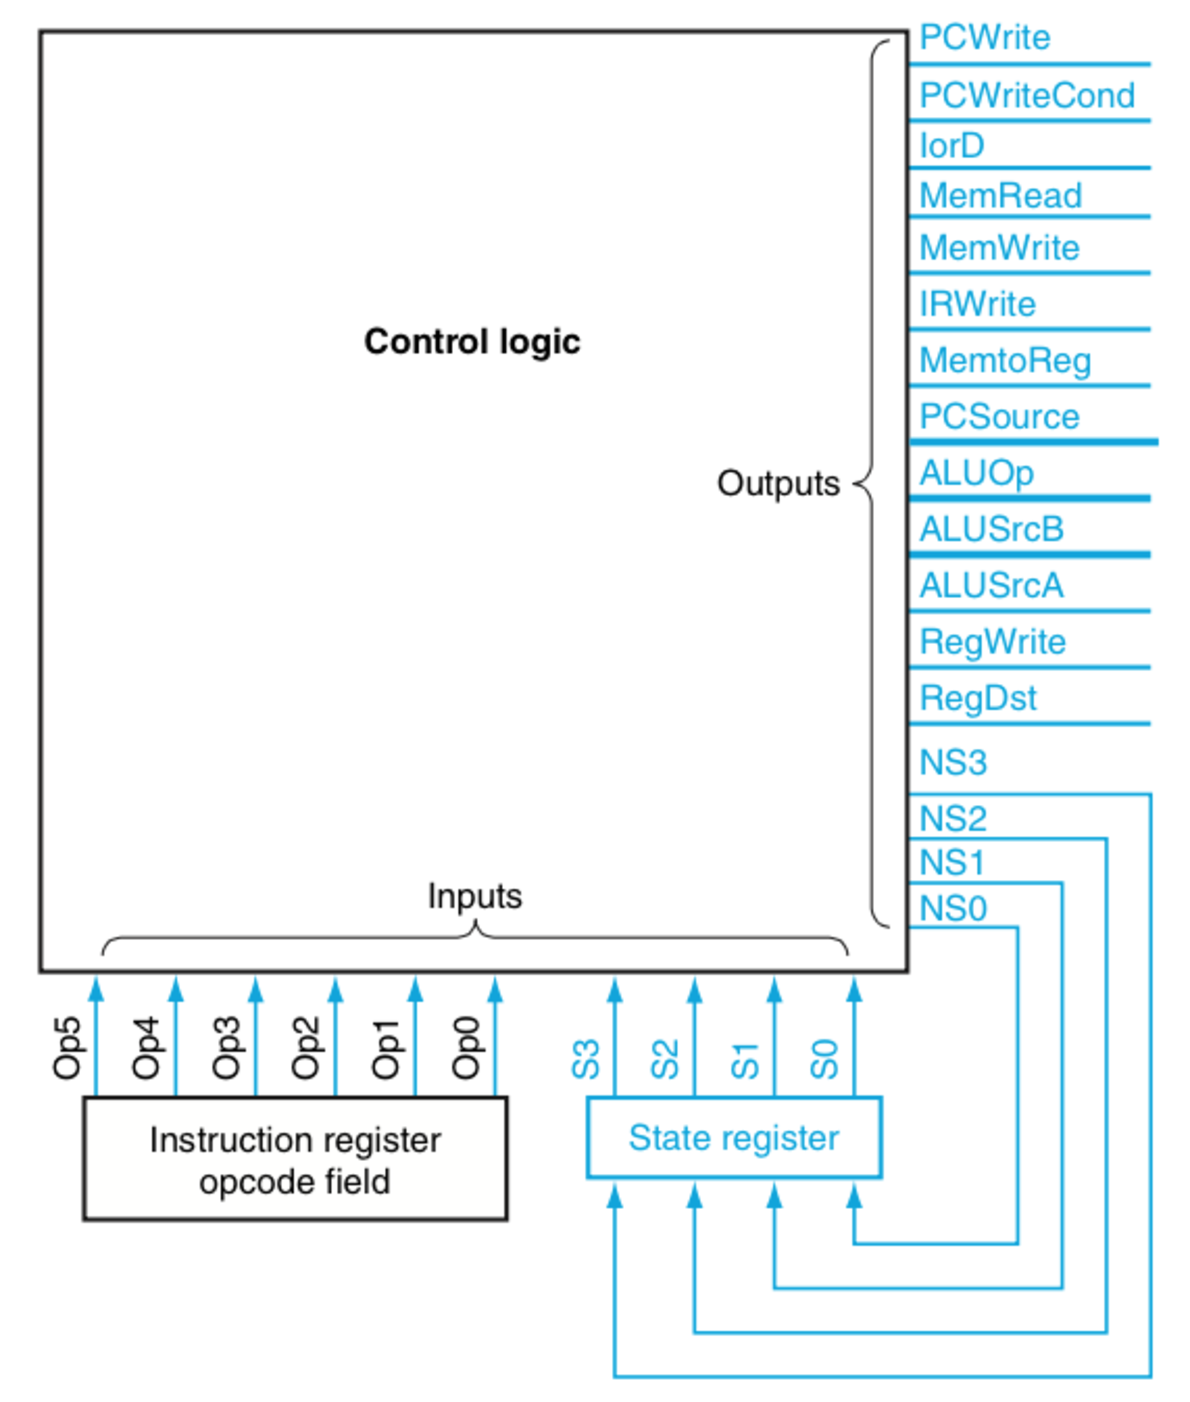
\includegraphics[width=4in]{./pics/control-logic-multi-cycle-processor}
\caption{A sequential circuit representing the FSM for the control unit of the multi-cycle {\it MIPS} processor \cite{Patterson2005a}. Its circuit topology has the canonical structure of sequential circuits shown in Figure \ref{fig:canonicalsequentiallogiccircuit}. The state register provide the state storage, and the control logic includes the next state logic and the output logic circuits needed to implement the FSM for the control unit of the processor.}
\label{fig:controllogicmulticycleprocessor}
\end{figure}
%	Figure D.3.2, pp. D-10, \cite{Patterson2005a}

The combinational circuit {\it C} in Figure \ref{fig:canonicalsequentiallogiccircuit} or the control logic in Figure \ref{fig:controllogicmulticycleprocessor} can be implemented using standard cells\cite{Kang2003a,Rabaey2003,Weste2011}, a read-only memory (ROM) device, or a programmable logic array (PLA). The ROM device or PLA encodes the truth tables for the boolean functions in the combinational circuit {\it C}.

%%%%%%%%%%%%%%%%%%%%%%%%%%%%%%%%%%%%%%%%%%%
\subsection{Advantages and Disadvantages of Multi-Cycle Processor Design}
\label{ssec:AdvantagesandDisadvantagesofMultiCycleProcessorDesign}

The advantage of the multi-cycle processor design over the microarchitecture for the single-cycle microarchitecture is the lower amount of hardware resources that are required in the datapath. From Equation \ref{eqn:ironlaw}, we can relatively compare the performance of the multi-cycle processor with the single-cycle processor. The CPI for the multi-cycle processor is higher than that of the single-cycle processor, since the multi-cycle processor takes multiple cycles to complete executing each instruction. However, the multi-cycle processor has a lower clock cycle period. If the normalized decrease in the clock period of the multi-cycle processor is relatively greater than the normalized increase in the CPI of the multi-cycle processor, the multi-cycle processor would have better performance than the single-cycle processor.




%%%%%%%%%%%%%%%%%%%%%%%%%%%%%%%%%%%%%%%%%%%
\subsection{Microprogramming}
\label{ssec:Microprogramming}

%In contemporary processors, there are ISAs that include more than 100 instructions, and these instructions can have clock cycle latencies ranging from 1 to 20 CPI. Therefore, manually detailing the control signals in a schematic of the VLSI circuit implementation of a microarchitecture is error prone. Likewise, a FSM representation of the control unit of a processor would be cumbersome to manually describe, too. There would be too many states (i.e., more than 1000 states) in the FSM representation. This means that it would be very difficult to verify such large FSMs \cite{Patterson2005a}. \\

Contemporary processors implement ISAs that include more than 100 instructions, and these instructions can have clock cycle latencies ranging from 1 to 20 CPI. Therefore, manually detailing the control signals in a schematic of the VLSI circuit implementation of a microarchitecture is error prone. Likewise, a FSM representation of the control unit of a processor would be cumbersome to manually describe too. There would be too many states (i.e., more than 1000 states) in the FSM representation. This means that it would be very difficult to verify such large FSMs \cite{Patterson2005a}. \\

Therefore, microprogramming is used to address this processor design challenge by treating each set of control signals as a microinstruction (or low-level control instruction) that can be executed by the datapath. This instruction would represent a state in the FSM for the control unit. That is, for each state in the FSM of the control unit, represent the output control signals from that state as a microinstruction to be executed in the datapath. It allows a set of (datapath) control signals to be symbolically represented as a microprogram, which consists of multiple microinstructions. Since many instructions in an ISA, such as the {\it MIPS} ISA, would share common sequences of microinstructions, a lot of code reuse of these common sequences (or microcode) occurs. Representing control signals as microcode/microprograms instead of wires, buses, and digital circuits allow the design of a microarchitecture to have a simpler control path \cite{Patterson2005a}. \\





















%%%%%%%%%%%%%%%%%%%%%%%%%%%%%%%%%%%%%%%%%
%	Pipeline Processor Design
%	This is written by Zhiyang Ong as a template for writing reports.

%	The MIT License (MIT)

%	Copyright (c) <2014> <Zhiyang Ong>

%	Permission is hereby granted, free of charge, to any person obtaining a copy of this software and associated documentation files (the "Software"), to deal in the Software without restriction, including without limitation the rights to use, copy, modify, merge, publish, distribute, sublicense, and/or sell copies of the Software, and to permit persons to whom the Software is furnished to do so, subject to the following conditions:

%	The above copyright notice and this permission notice shall be included in all copies or substantial portions of the Software.

%	THE SOFTWARE IS PROVIDED "AS IS", WITHOUT WARRANTY OF ANY KIND, EXPRESS OR IMPLIED, INCLUDING BUT NOT LIMITED TO THE WARRANTIES OF MERCHANTABILITY, FITNESS FOR A PARTICULAR PURPOSE AND NONINFRINGEMENT. IN NO EVENT SHALL THE AUTHORS OR COPYRIGHT HOLDERS BE LIABLE FOR ANY CLAIM, DAMAGES OR OTHER LIABILITY, WHETHER IN AN ACTION OF CONTRACT, TORT OR OTHERWISE, ARISING FROM, OUT OF OR IN CONNECTION WITH THE SOFTWARE OR THE USE OR OTHER DEALINGS IN THE SOFTWARE.

%	Email address: echo "cukj -wb- 23wU4X5M589 TROJANS cqkH wiuz2y 0f Mw Stanford" | awk '{ sub("23wU4X5M589","F.d_c_b. ") sub("Stanford","d0mA1n"); print $5, $2, $8; for (i=1; i<=1; i++) print "6\b"; print $9, $7, $6 }' | sed y/kqcbuHwM62z/gnotrzadqmC/ | tr 'q' ' ' | tr -d [:cntrl:] | tr -d 'ir' | tr y "\n"

%%%%%%%%%%%%%%%%%%%%%%%%%%%%%%%%%%%%%%%%%%%%%%


%%%%%%%%%%%%%%%%%%%%%%%%%%%%%%%%%%%%%%%%%%%
\section{Pipelined Processor Design}
\label{sec:PipelinedProcessorDesign}

%    Hennessy2012
%    Appendix C (pipelining)

%    Hennessy2007
%    Appendix A (pipelining)

%    Hennessy2003
%    Appendix A (pipelining)

%	6.27, microarch; 6.32; 6.36; 6.41; 6.42
%	3e, figure 6.17, microarchitecture, datapath



\begin{figure}[h]
\centering 
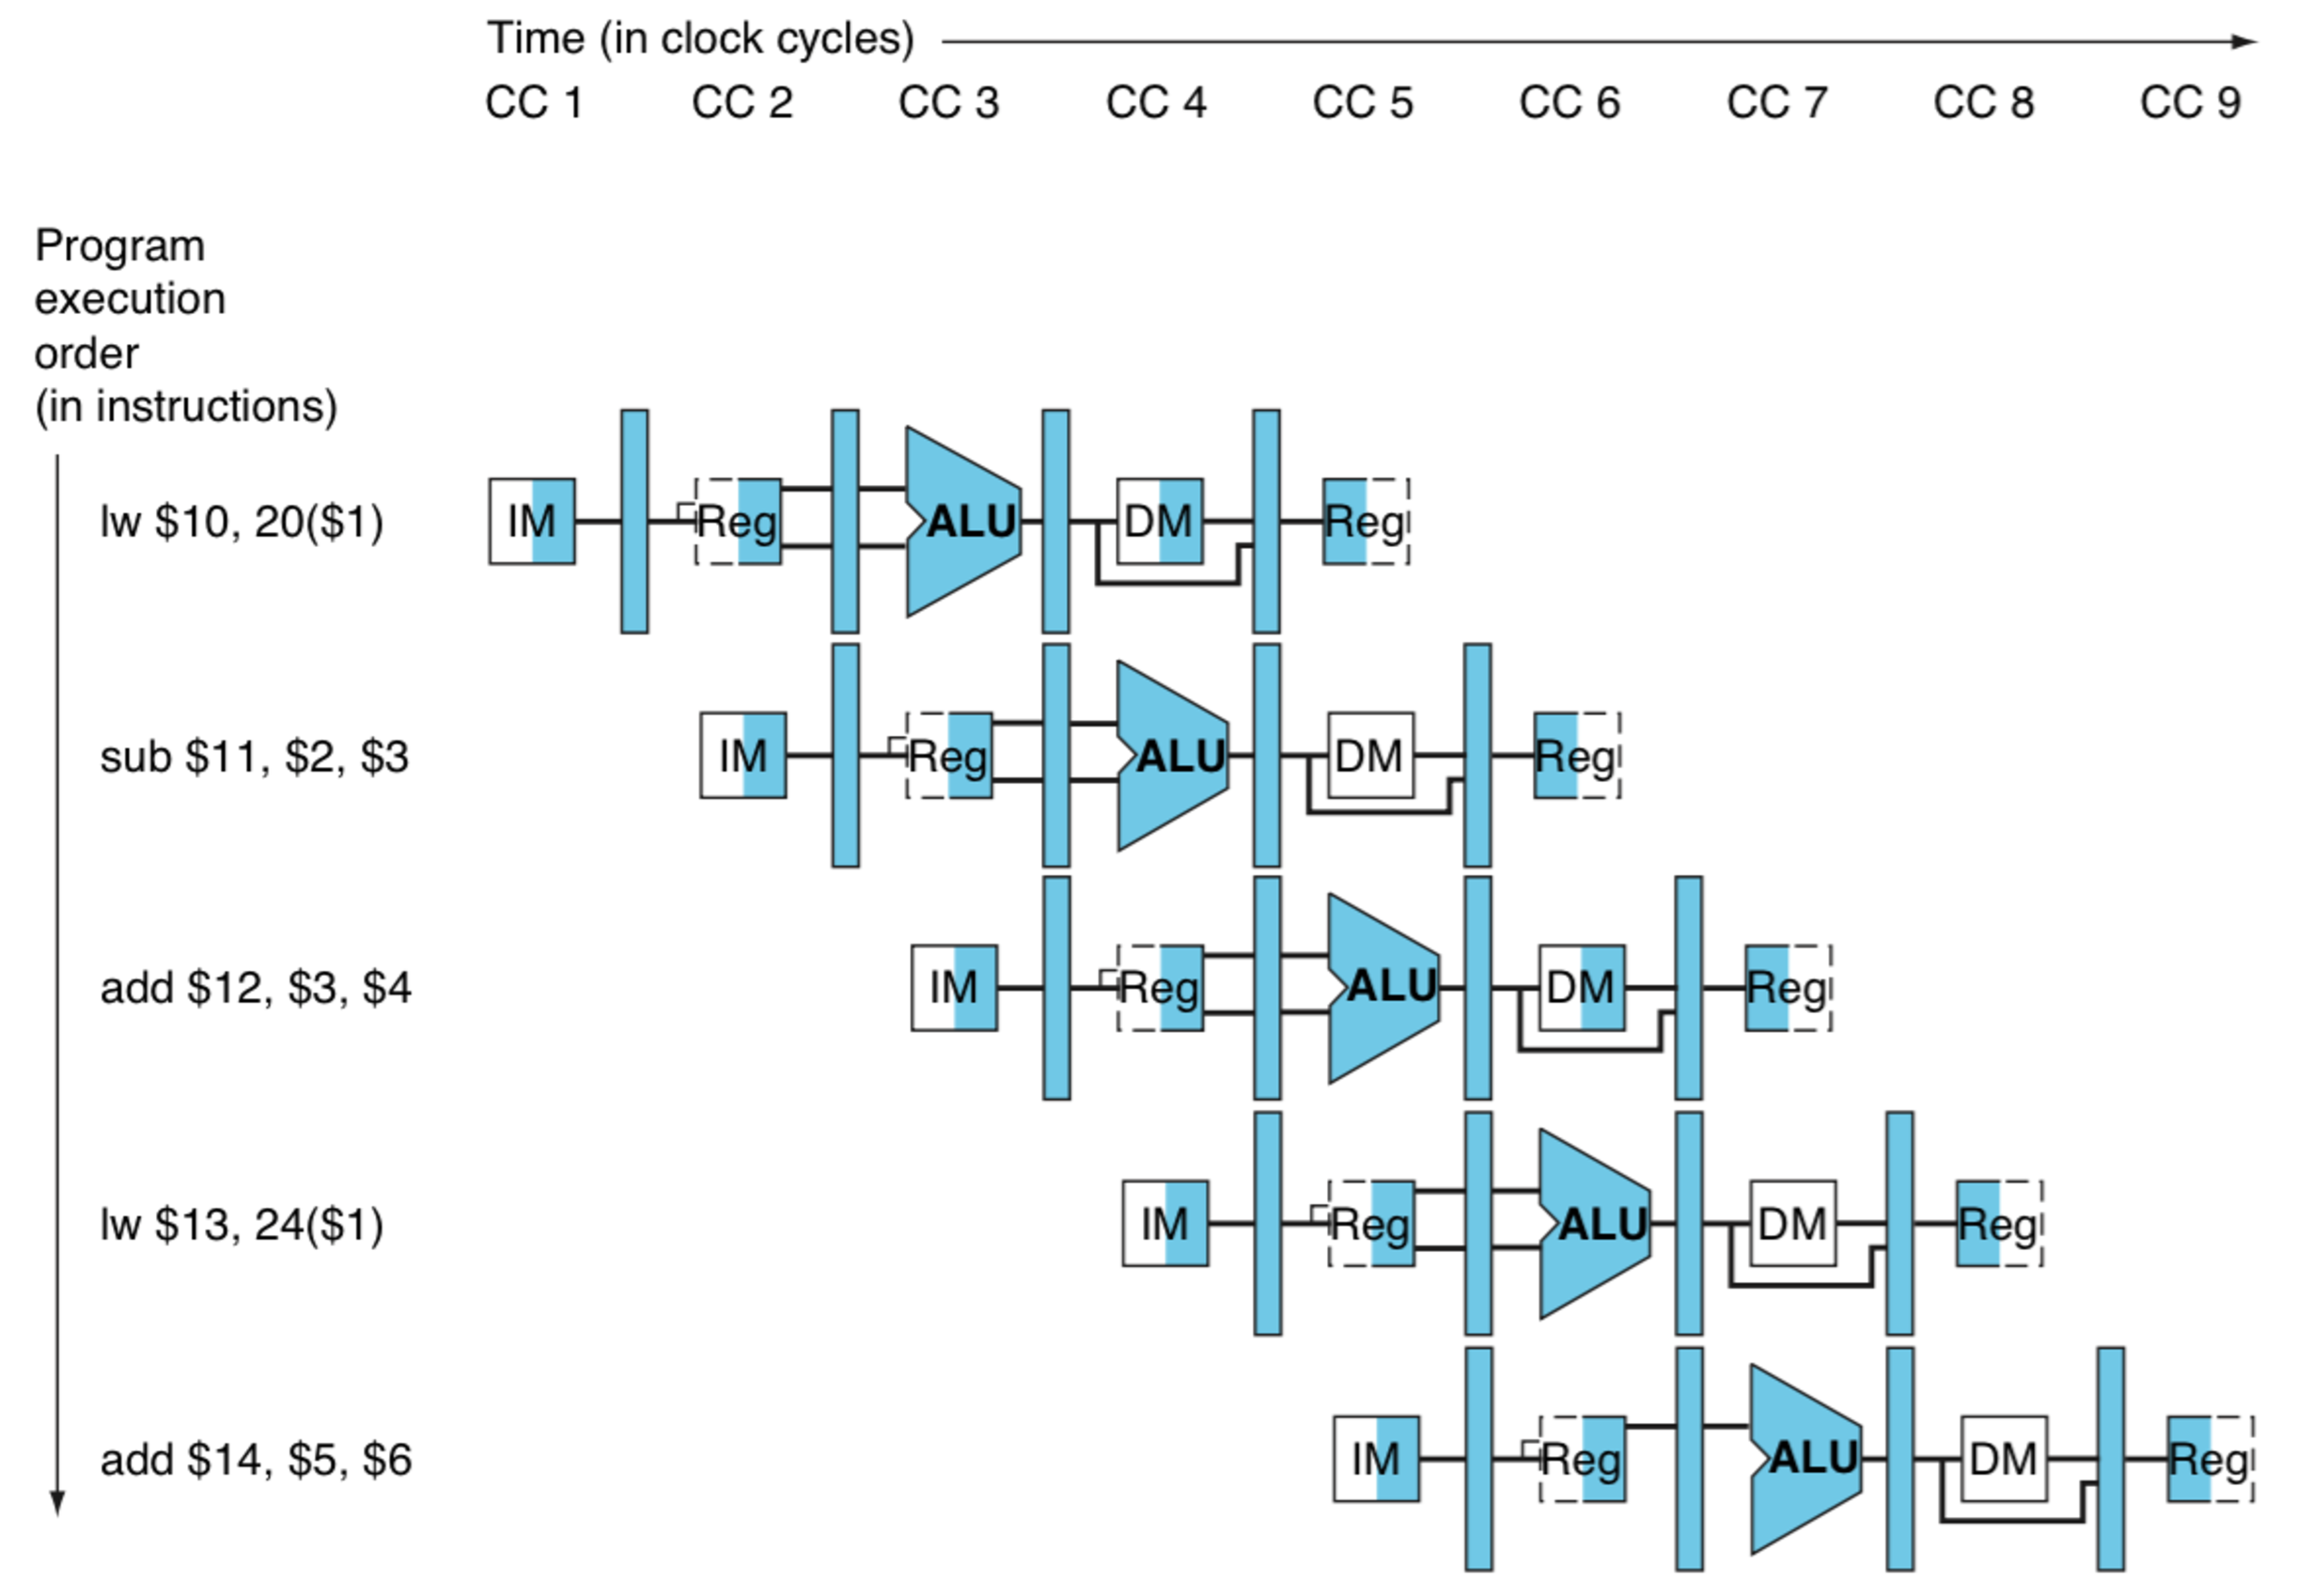
\includegraphics[width=6in]{./pics/pipelined-processor-pipelining}
\caption{A diagram of the datapath pipeline of the pipelined {\it MIPS} processor that shows the order of instruction execution for a sequence of five {\it MIPS} instructions. This datapath pipeline shows that each instruction would take at at least 5 clock cycles to execute \cite{Patterson2012}.}
\label{fig:pipelinedprocessorpipelining}
\end{figure}
%    pipeline diagram, 
%    Figure 6.19, Patterson2005, pp. 397
%    Figure 4.43, Patterson2012, pp. 357

Pipelining is a microarchitecture design technique that overlaps instructions, so that more hardware resources (or datapath components) in the datapath pipeline can be utilized. This allows computer programs to execute faster, and improve the performance of the pipelined processor. Figure \ref{fig:pipelinedprocessorpipelining} shows how the datapath of a pipelined {\it MIPS} processor can be pipelined to utilize more datapath components in each clock cycle. This pipelined {\it MIPS} processor fetches a new instruction every clock cycle, and each pipelined stage of the processor is processed in a clock cycle. At the next clock cycle, a given stage in the pipelined datapath would process the next instruction. An example of maximizing the usage of datapath components is shown in the fifth clock cycle, when all pipeline stages of the processor are being utilized. Therefore, pipelined processors are faster than multi-cycle processors, since the throughput of executing instructions is increased \cite{Patterson2012} to reduced the average execution time per instruction \cite{Hennessy2012}. \\

The performance speedup for a pipelined {\it MIPS} processor over an unpipelined {\it MIPS} processor is given as follows \cite{Hennessy2012}:\begin{equation}
\label{eqn:pipelinedprocessorspeedup}
{\rm performance\ speedup\ from\ pipelining} = \frac{\rm average\ execution\ time\ per\ unpipelined\ instruction}{\rm average\ execution\ time\ per\ pipelined\ instruction}
\end{equation}


\begin{figure}[h]
\centering 
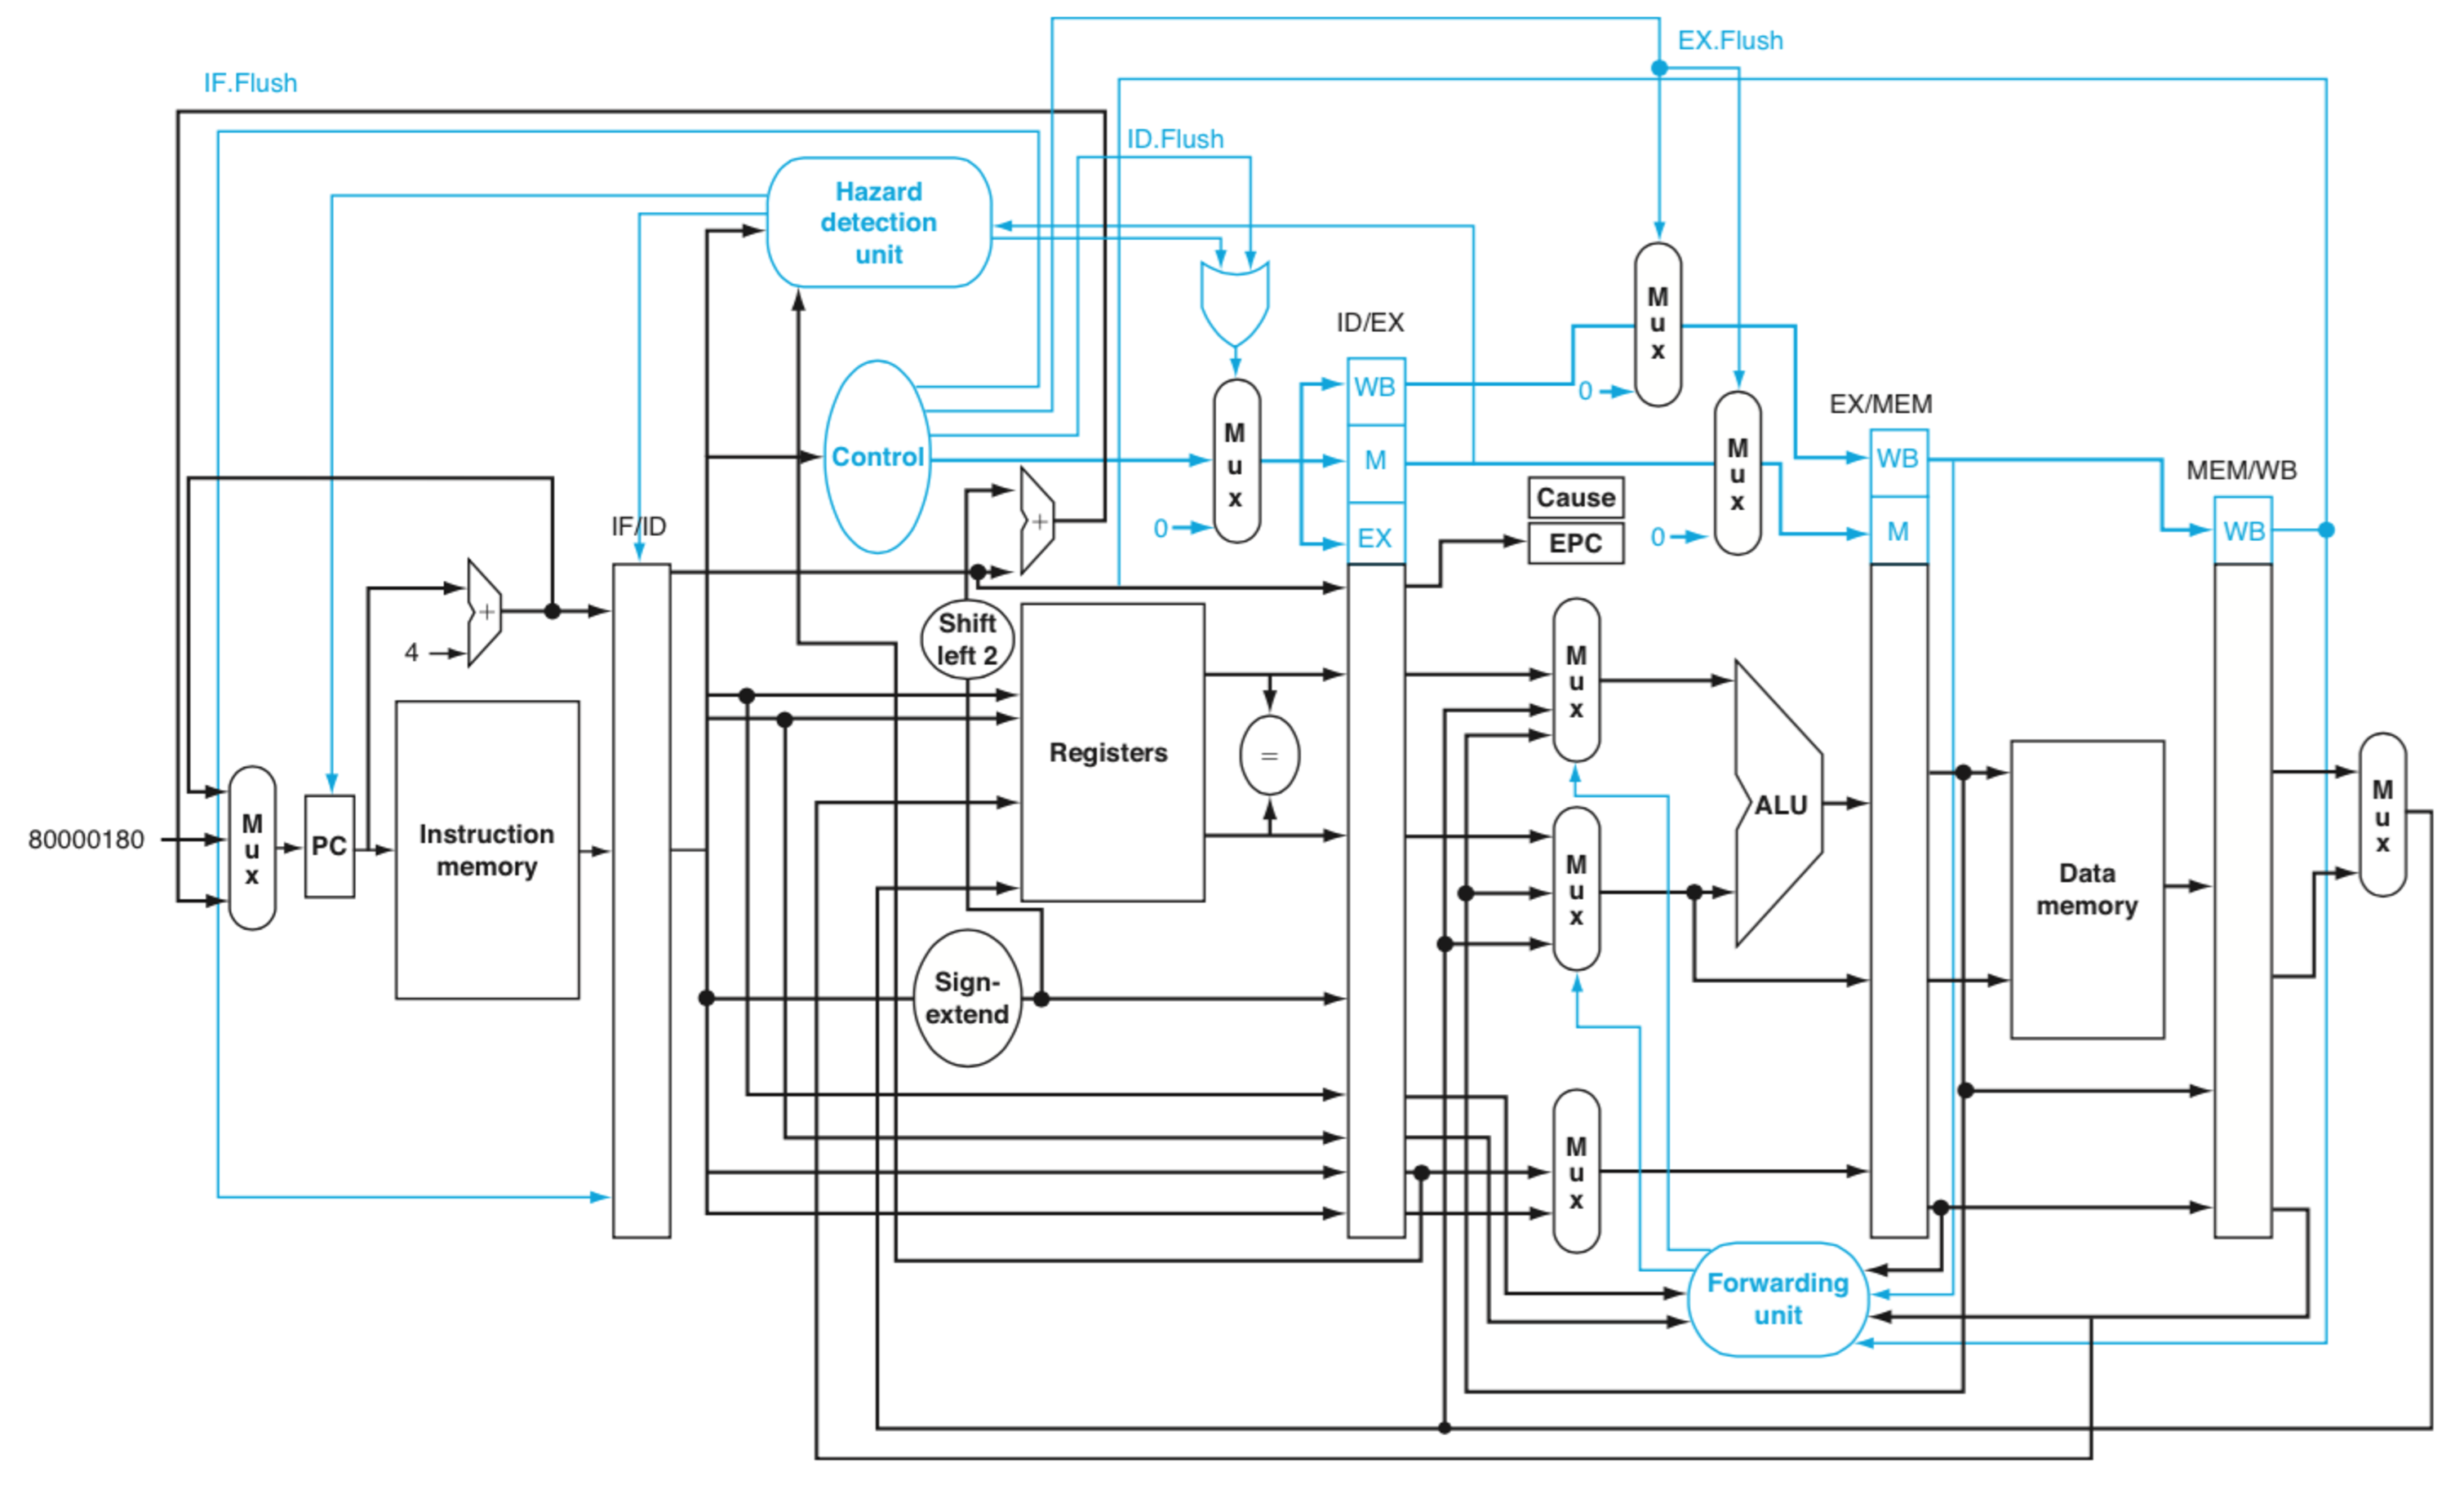
\includegraphics[width=6in]{./pics/pipelined-processor}
\caption{Microarchitecture of a pipelined {\it MIPS} processor that includes the datapath and the control path. It supports detection and handling of exceptions \cite{Patterson2012}.}
\label{fig:pipelinedprocessor}
\end{figure}
%    Datapath and control path 
%    Figure 6.42, Patterson2005, pp. 428
%    Figure 4.66, Patterson2012, pp. 387

%Figure \ref{fig:pipelinedprocessor} shows the microarchitecture of a pipelined {\it MIPS} processor that supports detection and handling of exceptions \cite{Patterson2012}. The pipelined stages of the pipelined {\it MIPS} processor's datapath are the same stages of the multi-cycle {\it MIPS} processor; see Section \ref{sec:MultiCycleProcessorDesign}. That is, the pipelined stages of the pipelined {\it MIPS} processor are: IF, ID, EX, MEM, and WB. In order to execute each pipelined stage in a clock cycle, pipelined registers are placed between pipelined stages to ensure that each pipelined stage will execute in one clock cycle.
Figure \ref{fig:pipelinedprocessor} shows the microarchitecture of a pipelined {\it MIPS} processor that supports detection and handling of exceptions \cite{Patterson2012}. The pipelined stages of the pipelined {\it MIPS} processor's datapath are the same stages of the multi-cycle {\it MIPS} processor; see Section \ref{sec:MultiCycleProcessorDesign}. That is, the pipelined stages of the pipelined {\it MIPS} processor are: IF, ID, EX, MEM, and WB. In order to execute each pipelined stage in a clock cycle, pipelined registers are placed between pipelined stages. \\

Pipeline hazards prevent the next instruction in the instruction sequence to execute during the clock cycle that it is supposed to. These pipeline hazards prevent the computer from achieving the ideal performance speedup. These hazards are categorized as follows \cite{Hennessy2012}: \vspace{-0.3cm}
\begin{enumerate} \itemsep -4pt
\item Structural hazards occur when multiple instructions need to use a datapath component in the same clock cycle. They prevent instructions from being overlapped in sequences, such that multiple instructions need to use a datapath component in the same clock cycle.
\item Data hazards occur when the computational results of an instruction are used or overwritten in subsequent instructions.
\item Control hazards occur when pipelined {\tt branch} and {\tt jump} instructions change the PC value.
\end{enumerate}


\begin{figure}[h]
\centering 
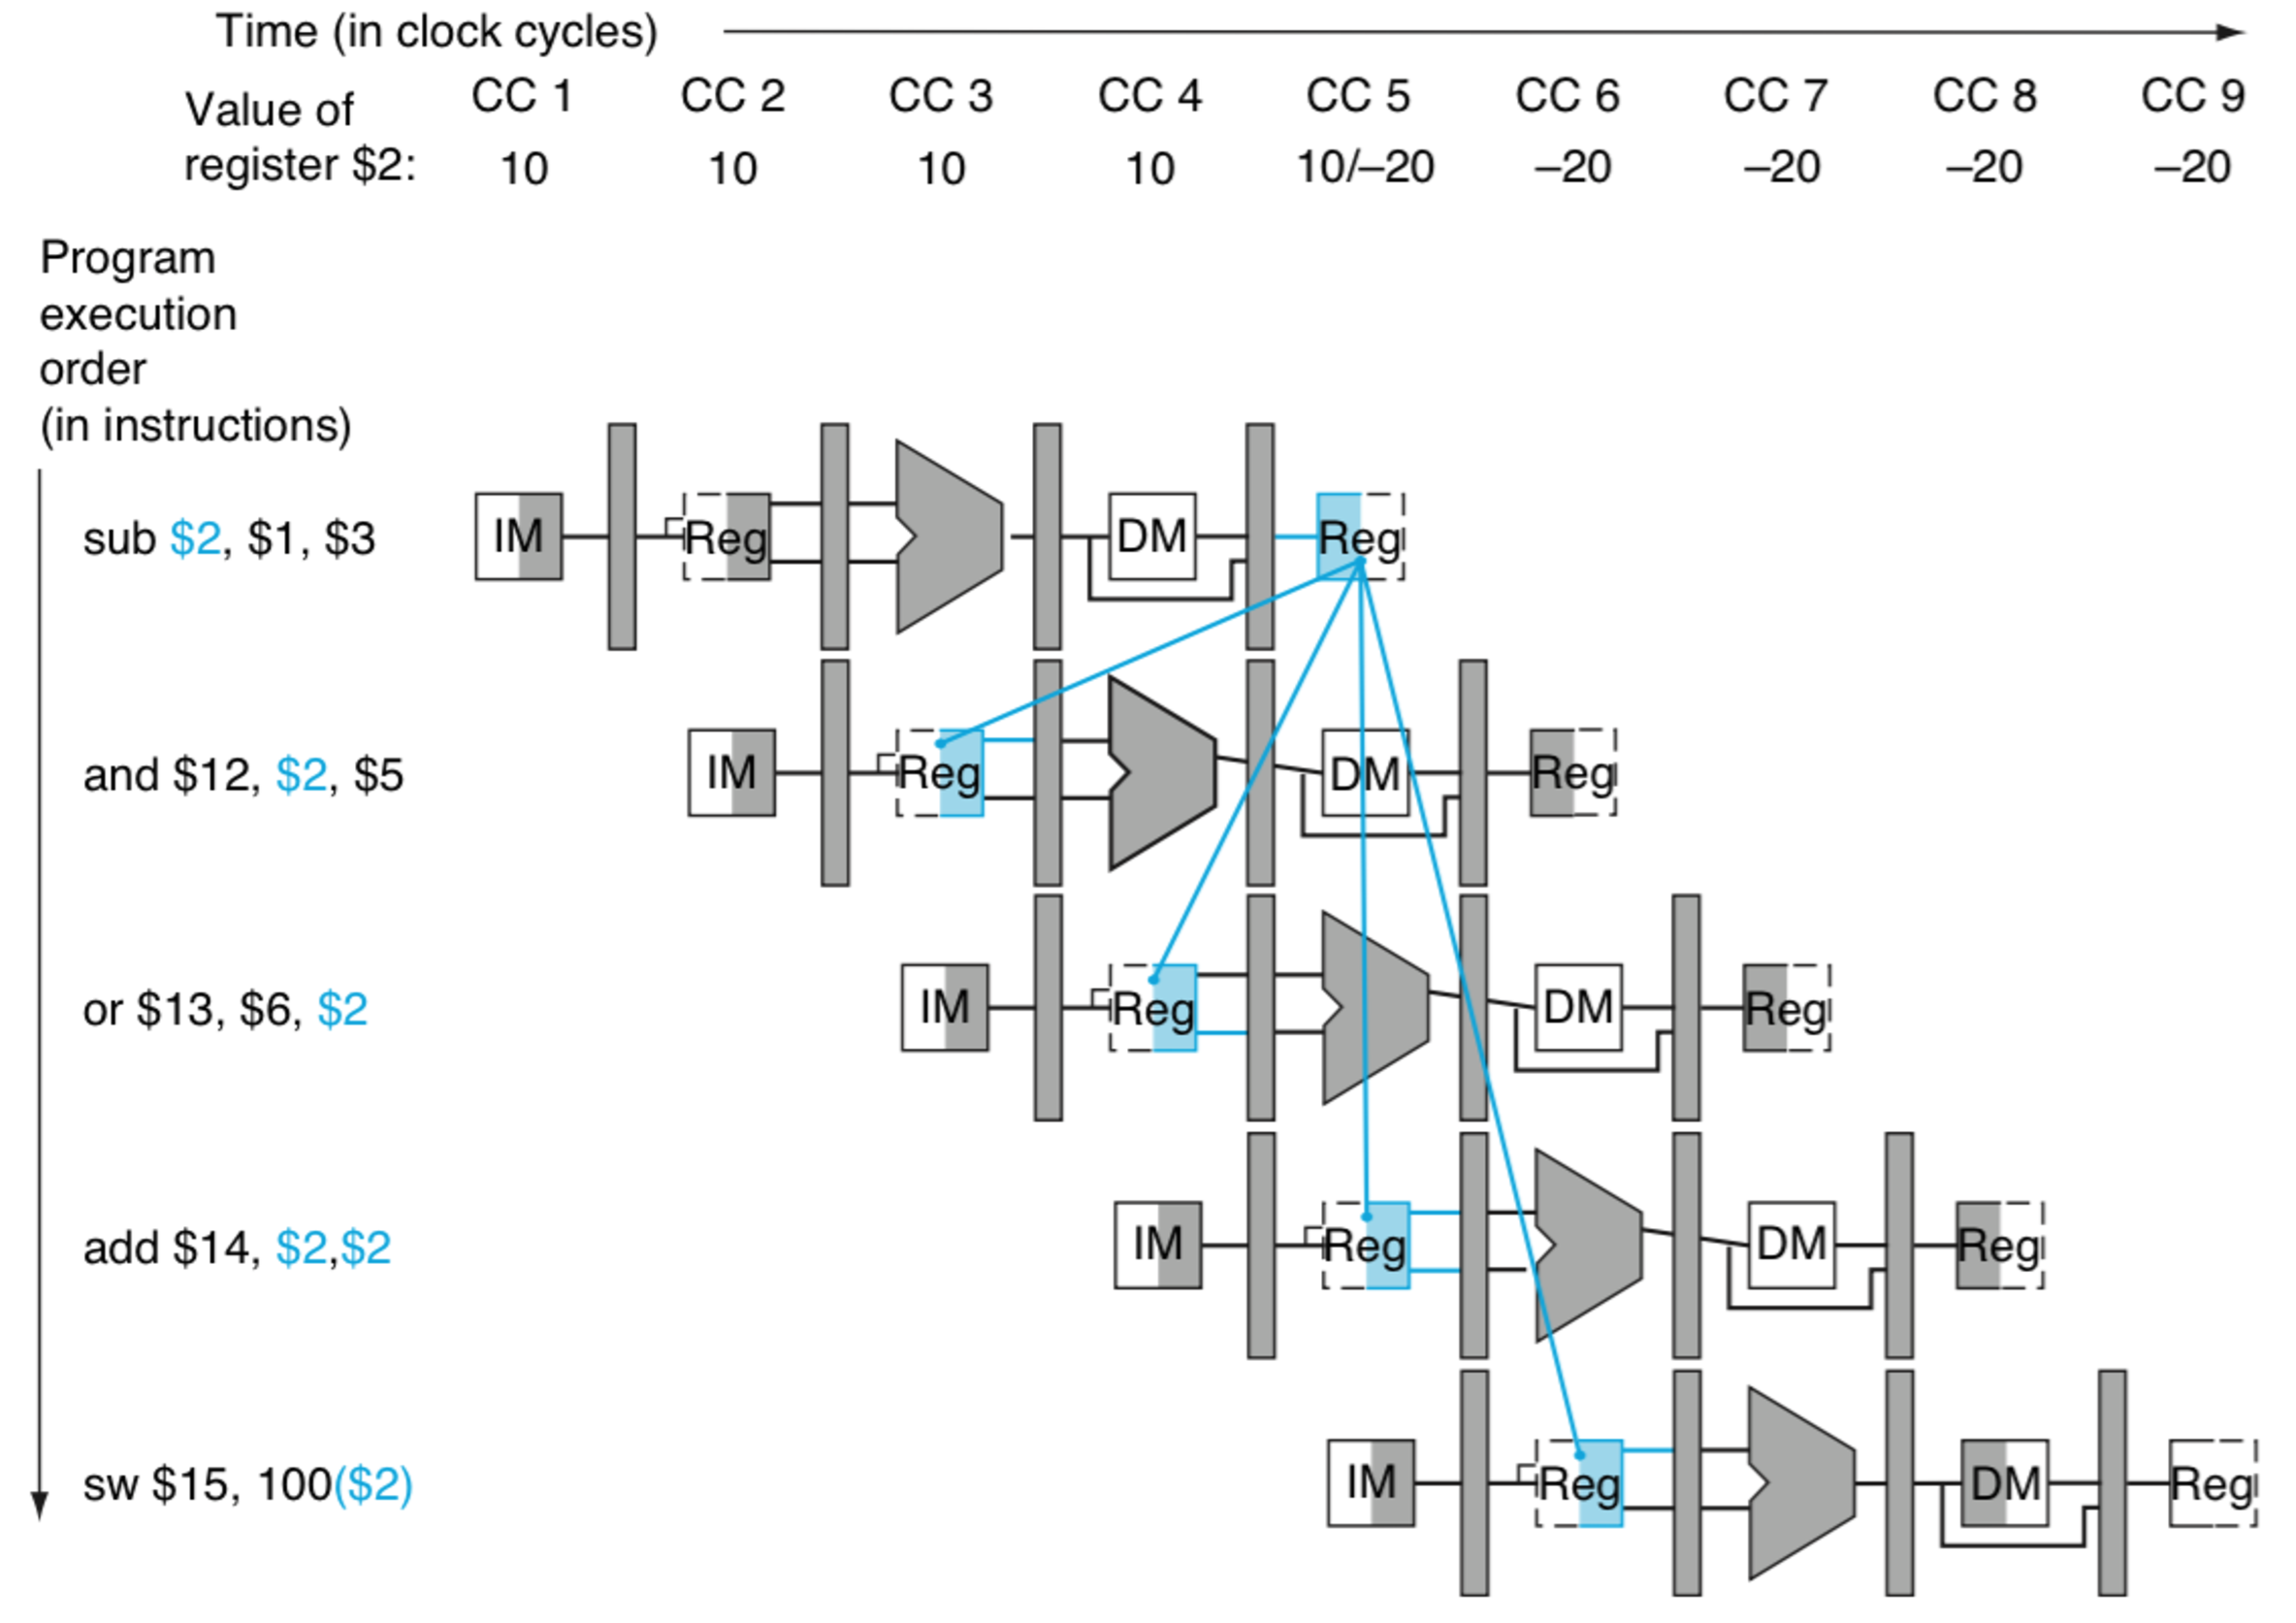
\includegraphics[width=6in]{./pics/pipelined-processor-raw-data-dependencies}
\caption{An example of Read-After-Write (RAW) data dependencies \cite{Hennessy2012,Shen2005a} between instructions in a snippet of a computer program \cite{Patterson2012}. There exists RAW data dependencies regarding register {\tt \$2} between the instruction {\tt sub \$2, \$1, \$3} and the following instructions: {\tt and \$12, \$2, \$5}; {\tt or \$13, \$6, \$2}; {\tt add \$14, \$2, \$2}; and {\tt sw \$15, 100(\$2)}. }
\label{fig:pipelinedprocessorrawdatadependencies}
\end{figure}
%    pipelined dependencies
%    Figure 6.28, Patterson2005, pp. 405
%    Figure 4.52, Patterson2012, pp. 364


\begin{figure}[h]
\centering 
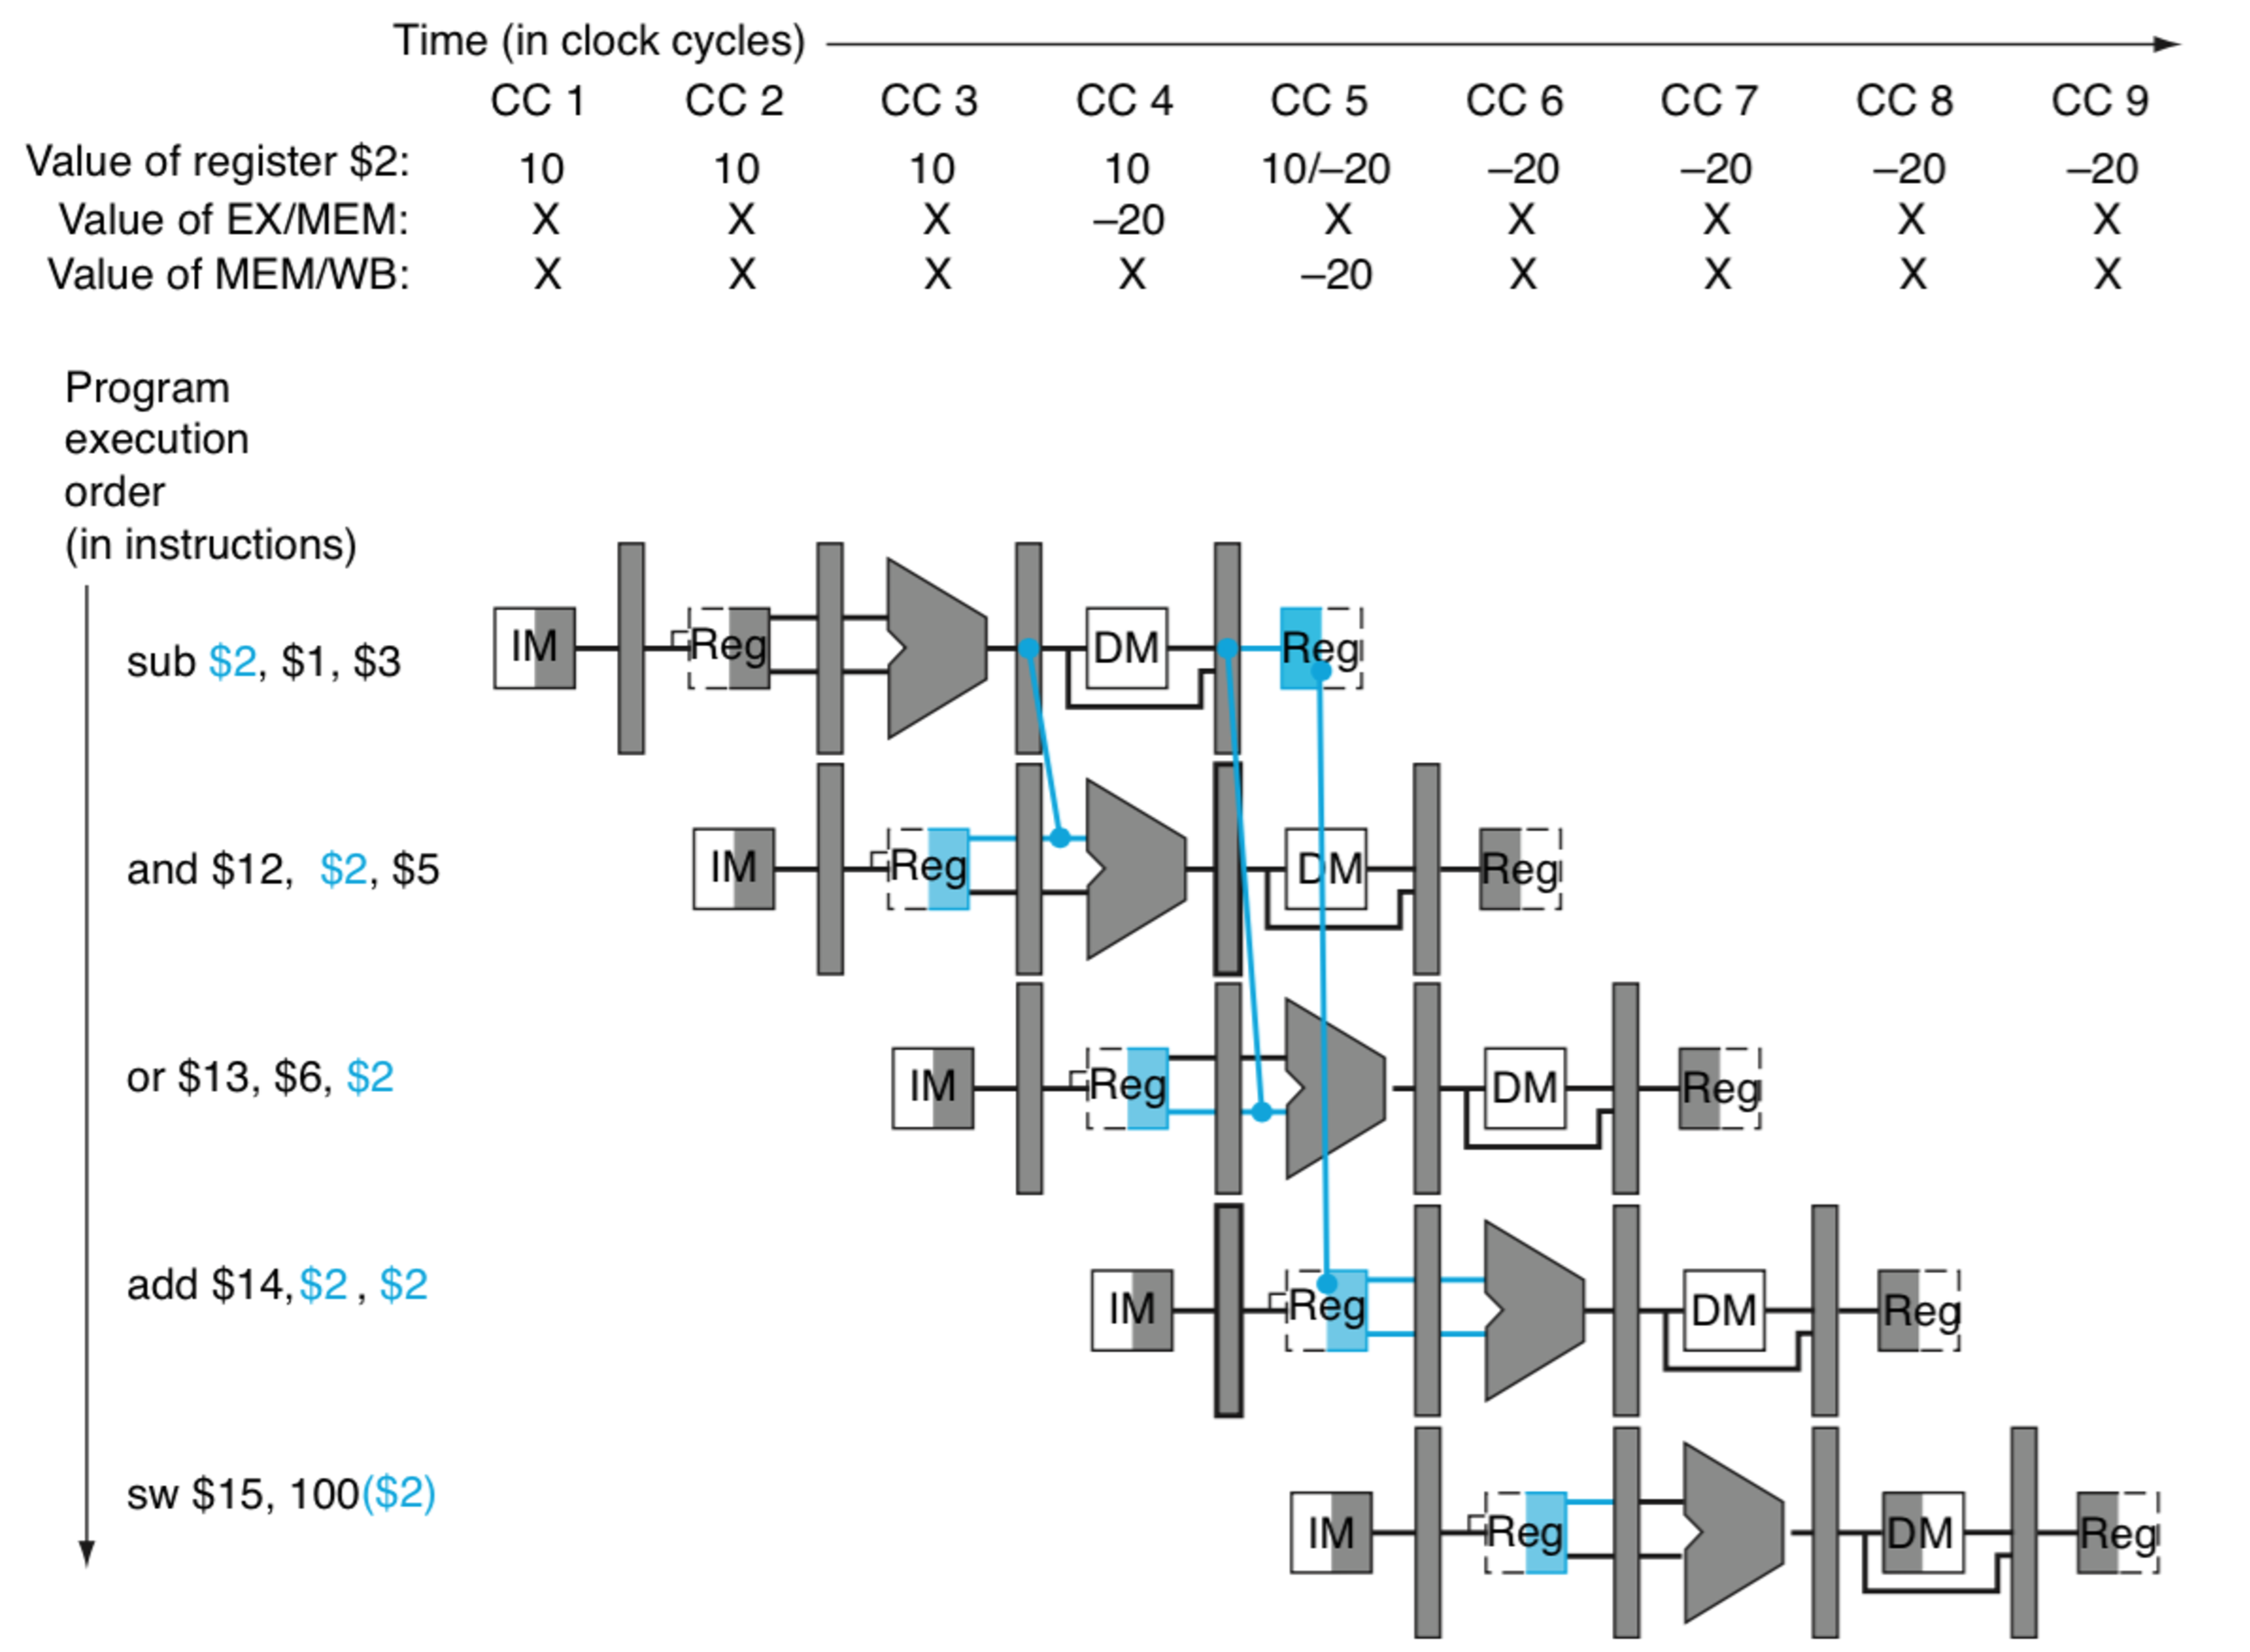
\includegraphics[width=6in]{./pics/pipelined-processor-forwarding}
\caption{An example of data dependencies that can be resolved by forwarding. This avoids data hazards \cite{Patterson2012}.}
\label{fig:pipelinedprocessorforwarding}
\end{figure}
%    dependencies resolution
%    Figure 6.29, Patterson2005, pp. 408
%    Figure 4.53, Patterson2012, pp. 367

%Figure \ref{fig:pipelinedprocessorrawdatadependencies} shows an example of Read-After-Write (RAW) data dependencies \cite{Hennessy2012,Shen2005a} between instructions in a snippet of a computer program \cite{Patterson2012}. There exist Read-After-Write (RAW) data dependencies \cite{Hennessy2012,Shen2005a} regarding register {\tt \$2} between the instruction {\tt sub \$2, \$1, \$3} and the following instructions: {\tt and \$12, \$2, \$5}; {\tt or \$13, \$6, \$2}; {\tt add \$14, \$2, \$2}; and {\tt sw \$15, 100(\$2)}. Figure \ref{fig:pipelinedprocessorforwarding} shows how these data dependencies can be resolved by forwarding dependent data from a datapath component to another datapath component in the same or next clock cycle. For example, there exists RAW data dependencies \cite{Hennessy2012,Shen2005a} regarding register {\tt \$2} between the instruction {\tt sub \$2, \$1, \$3} and the following instructions: {\tt and \$12, \$2, \$5}; {\tt or \$13, \$6, \$2}; and {\tt add \$14, \$2, \$2}. Therefore, forwarding is used to transfer the updated value of register {\tt \$2} to: the input of the ALU for the instruction {\tt and \$12, \$2, \$5}; the input of the ALU for the instruction {\tt or \$13, \$6, \$2}; and the register file at {\tt add \$14, \$2, \$2}. The RAW data dependency for register {\tt \$2} in last instruction {\tt sw \$15, 100(\$2)} will not cause a data hazard, since the value at register {\tt \$2} will be ready to be read from the register file at cycle six.
An extensive coverage of pipeline hazards is beyond the scope of this report. However, I will briefly address data dependencies and data hazards. Figure \ref{fig:pipelinedprocessorrawdatadependencies} shows an example of Read-After-Write (RAW) data dependencies \cite{Hennessy2012,Shen2005a} between instructions in a snippet of a computer program \cite{Patterson2012}. There exist Read-After-Write (RAW) data dependencies \cite{Hennessy2012,Shen2005a} regarding register {\tt \$2} between the instruction {\tt sub \$2, \$1, \$3} and the following instructions: {\tt and \$12, \$2, \$5}; {\tt or \$13, \$6, \$2}; {\tt add \$14, \$2, \$2}; and {\tt sw \$15, 100(\$2)}. Figure \ref{fig:pipelinedprocessorforwarding} shows how these data dependencies can be resolved by forwarding dependent data from a datapath component to another datapath component in the same or next clock cycle \cite{Patterson2012}. For example, there exists RAW data dependencies \cite{Hennessy2012,Shen2005a} regarding register {\tt \$2} between the instruction {\tt sub \$2, \$1, \$3} and the following instructions: {\tt and \$12, \$2, \$5}; {\tt or \$13, \$6, \$2}; and {\tt add \$14, \$2, \$2}. Therefore, forwarding is used to transfer the updated value of register {\tt \$2} to: the input of the ALU for the instruction {\tt and \$12, \$2, \$5}; the input of the ALU for the instruction {\tt or \$13, \$6, \$2}; and the register file at {\tt add \$14, \$2, \$2}. The RAW data dependency for register {\tt \$2} in last instruction {\tt sw \$15, 100(\$2)} will not cause a data hazard, since the value at register {\tt \$2} will be ready to be read from the register file at cycle six. \\


\begin{figure}[h]
\centering 
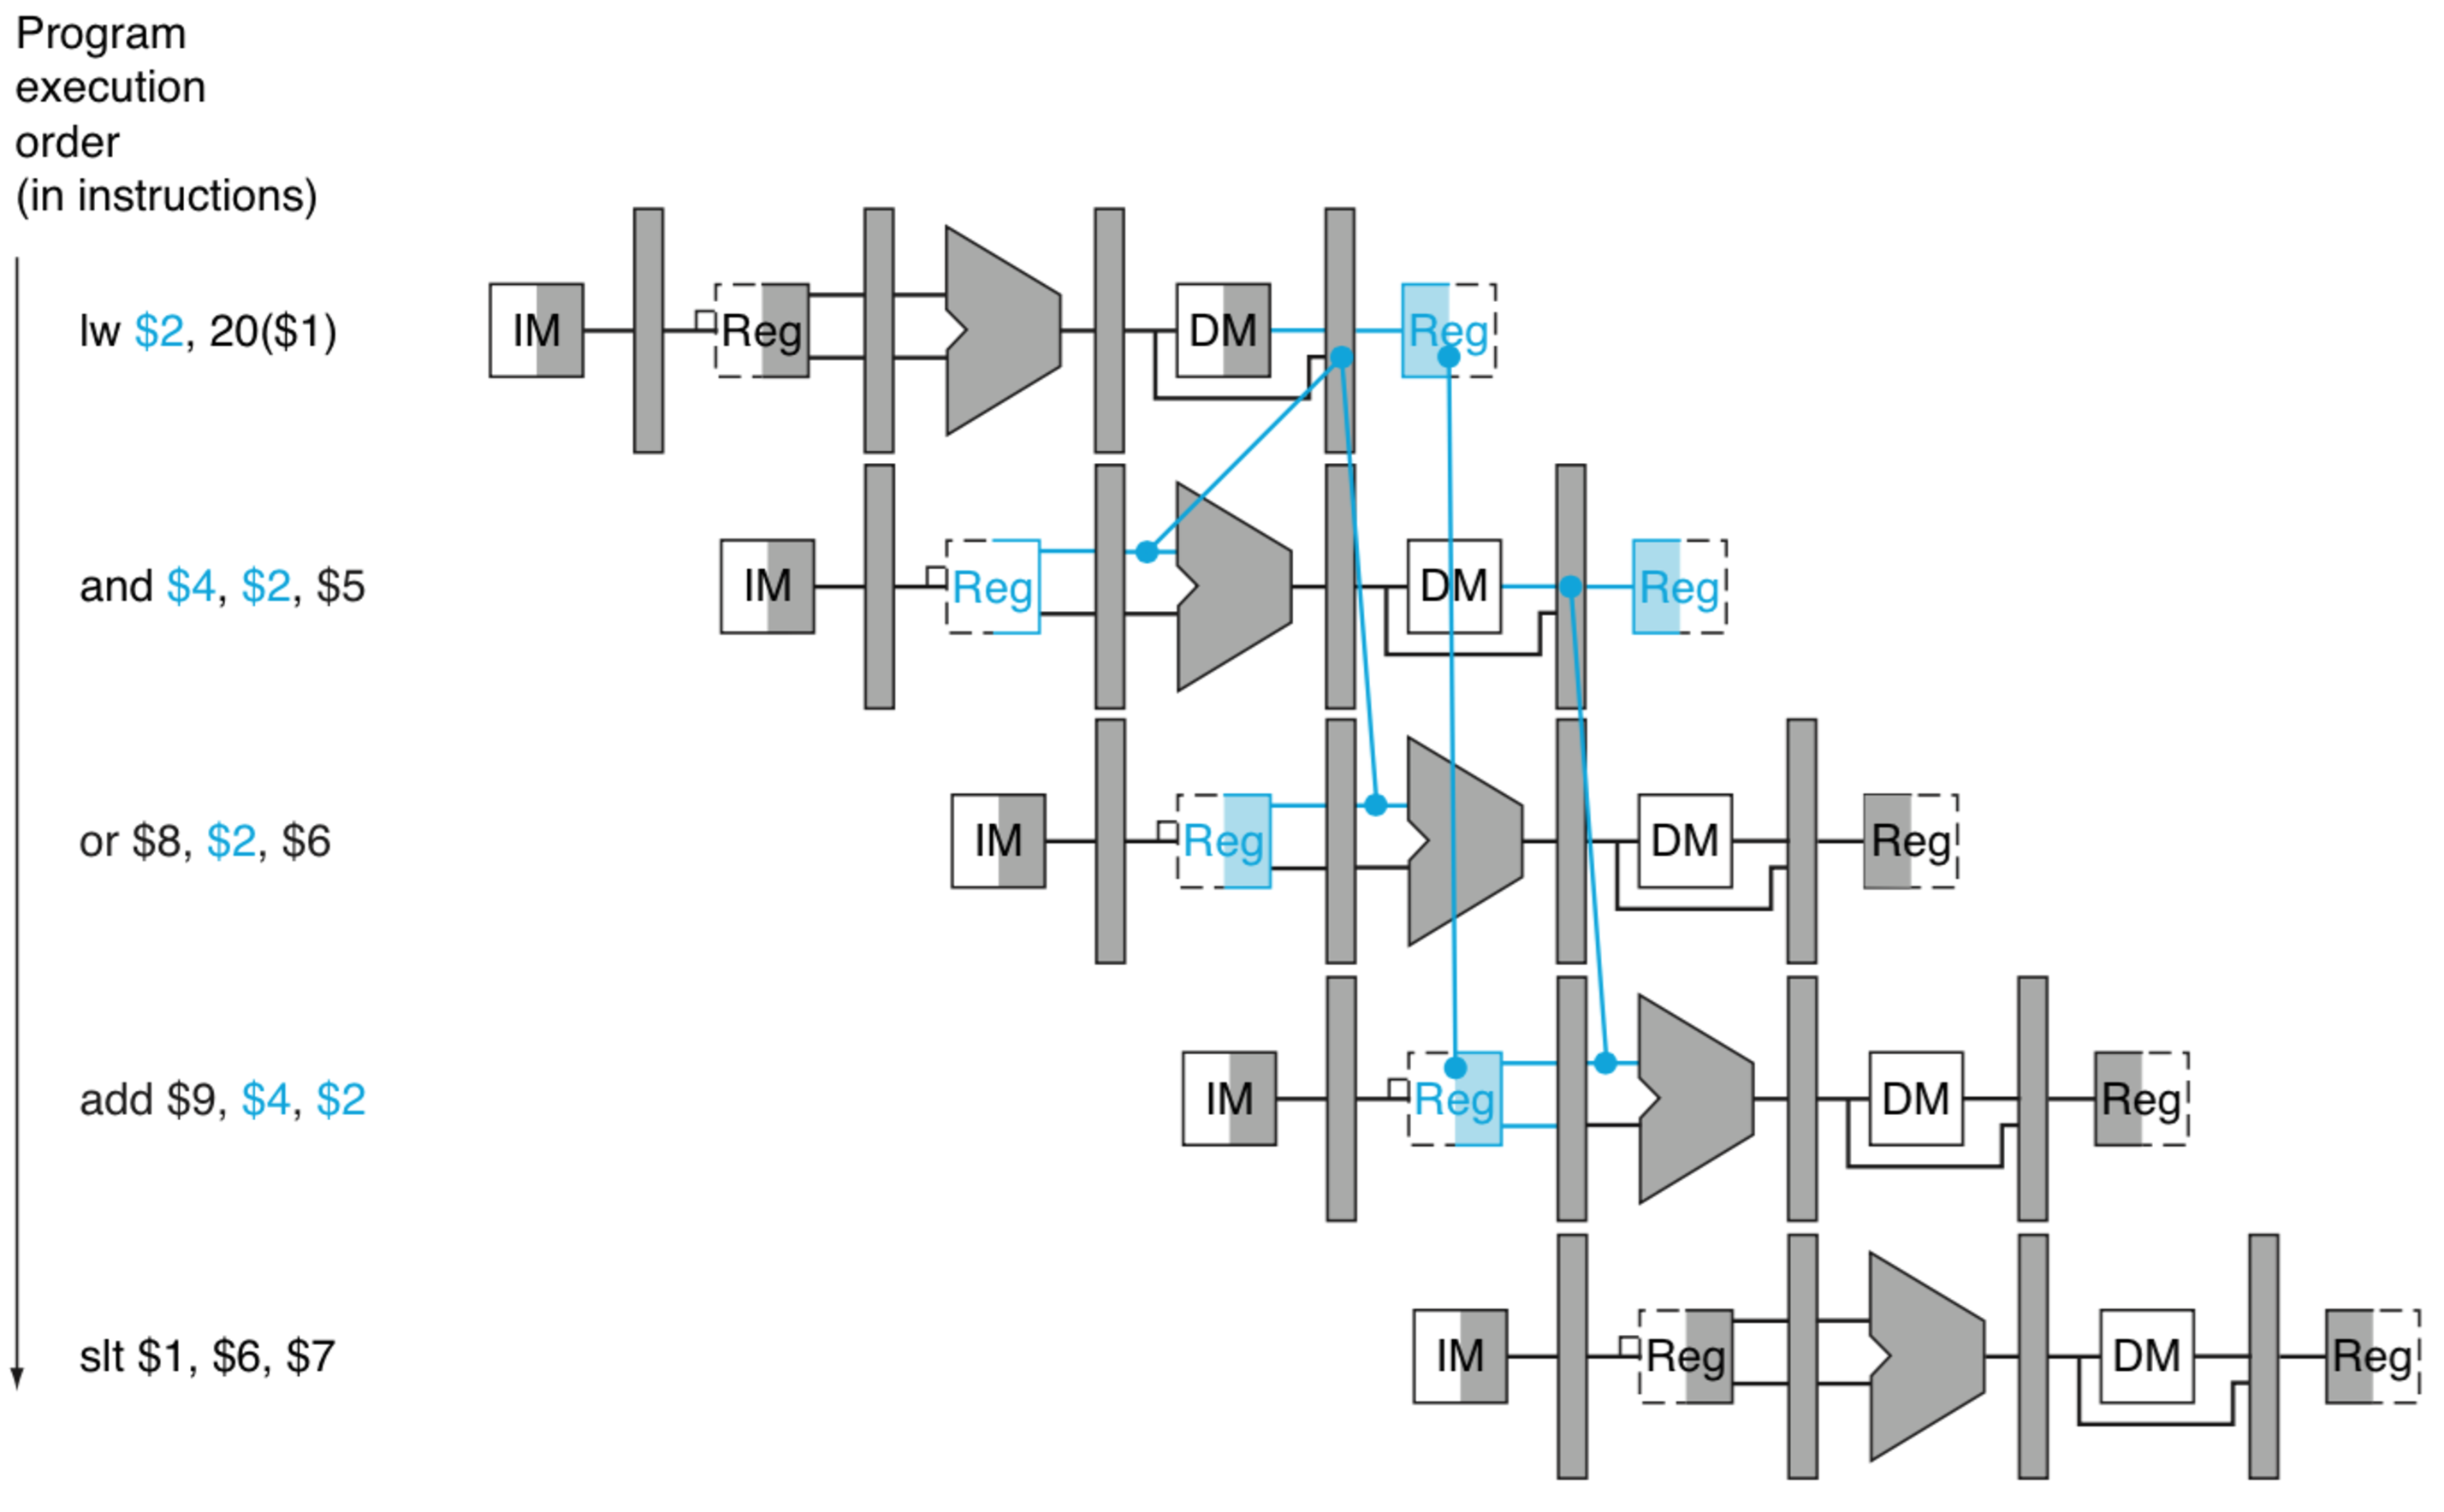
\includegraphics[width=6in]{./pics/pipelined-processor-data-hazards}
\caption{An example of data dependencies that cannot be resolved by forwarding and will cause data hazards \cite{Patterson2012}.}
\label{fig:pipelined-processor-data-hazards}
\end{figure}

\begin{figure}[h]
\centering 
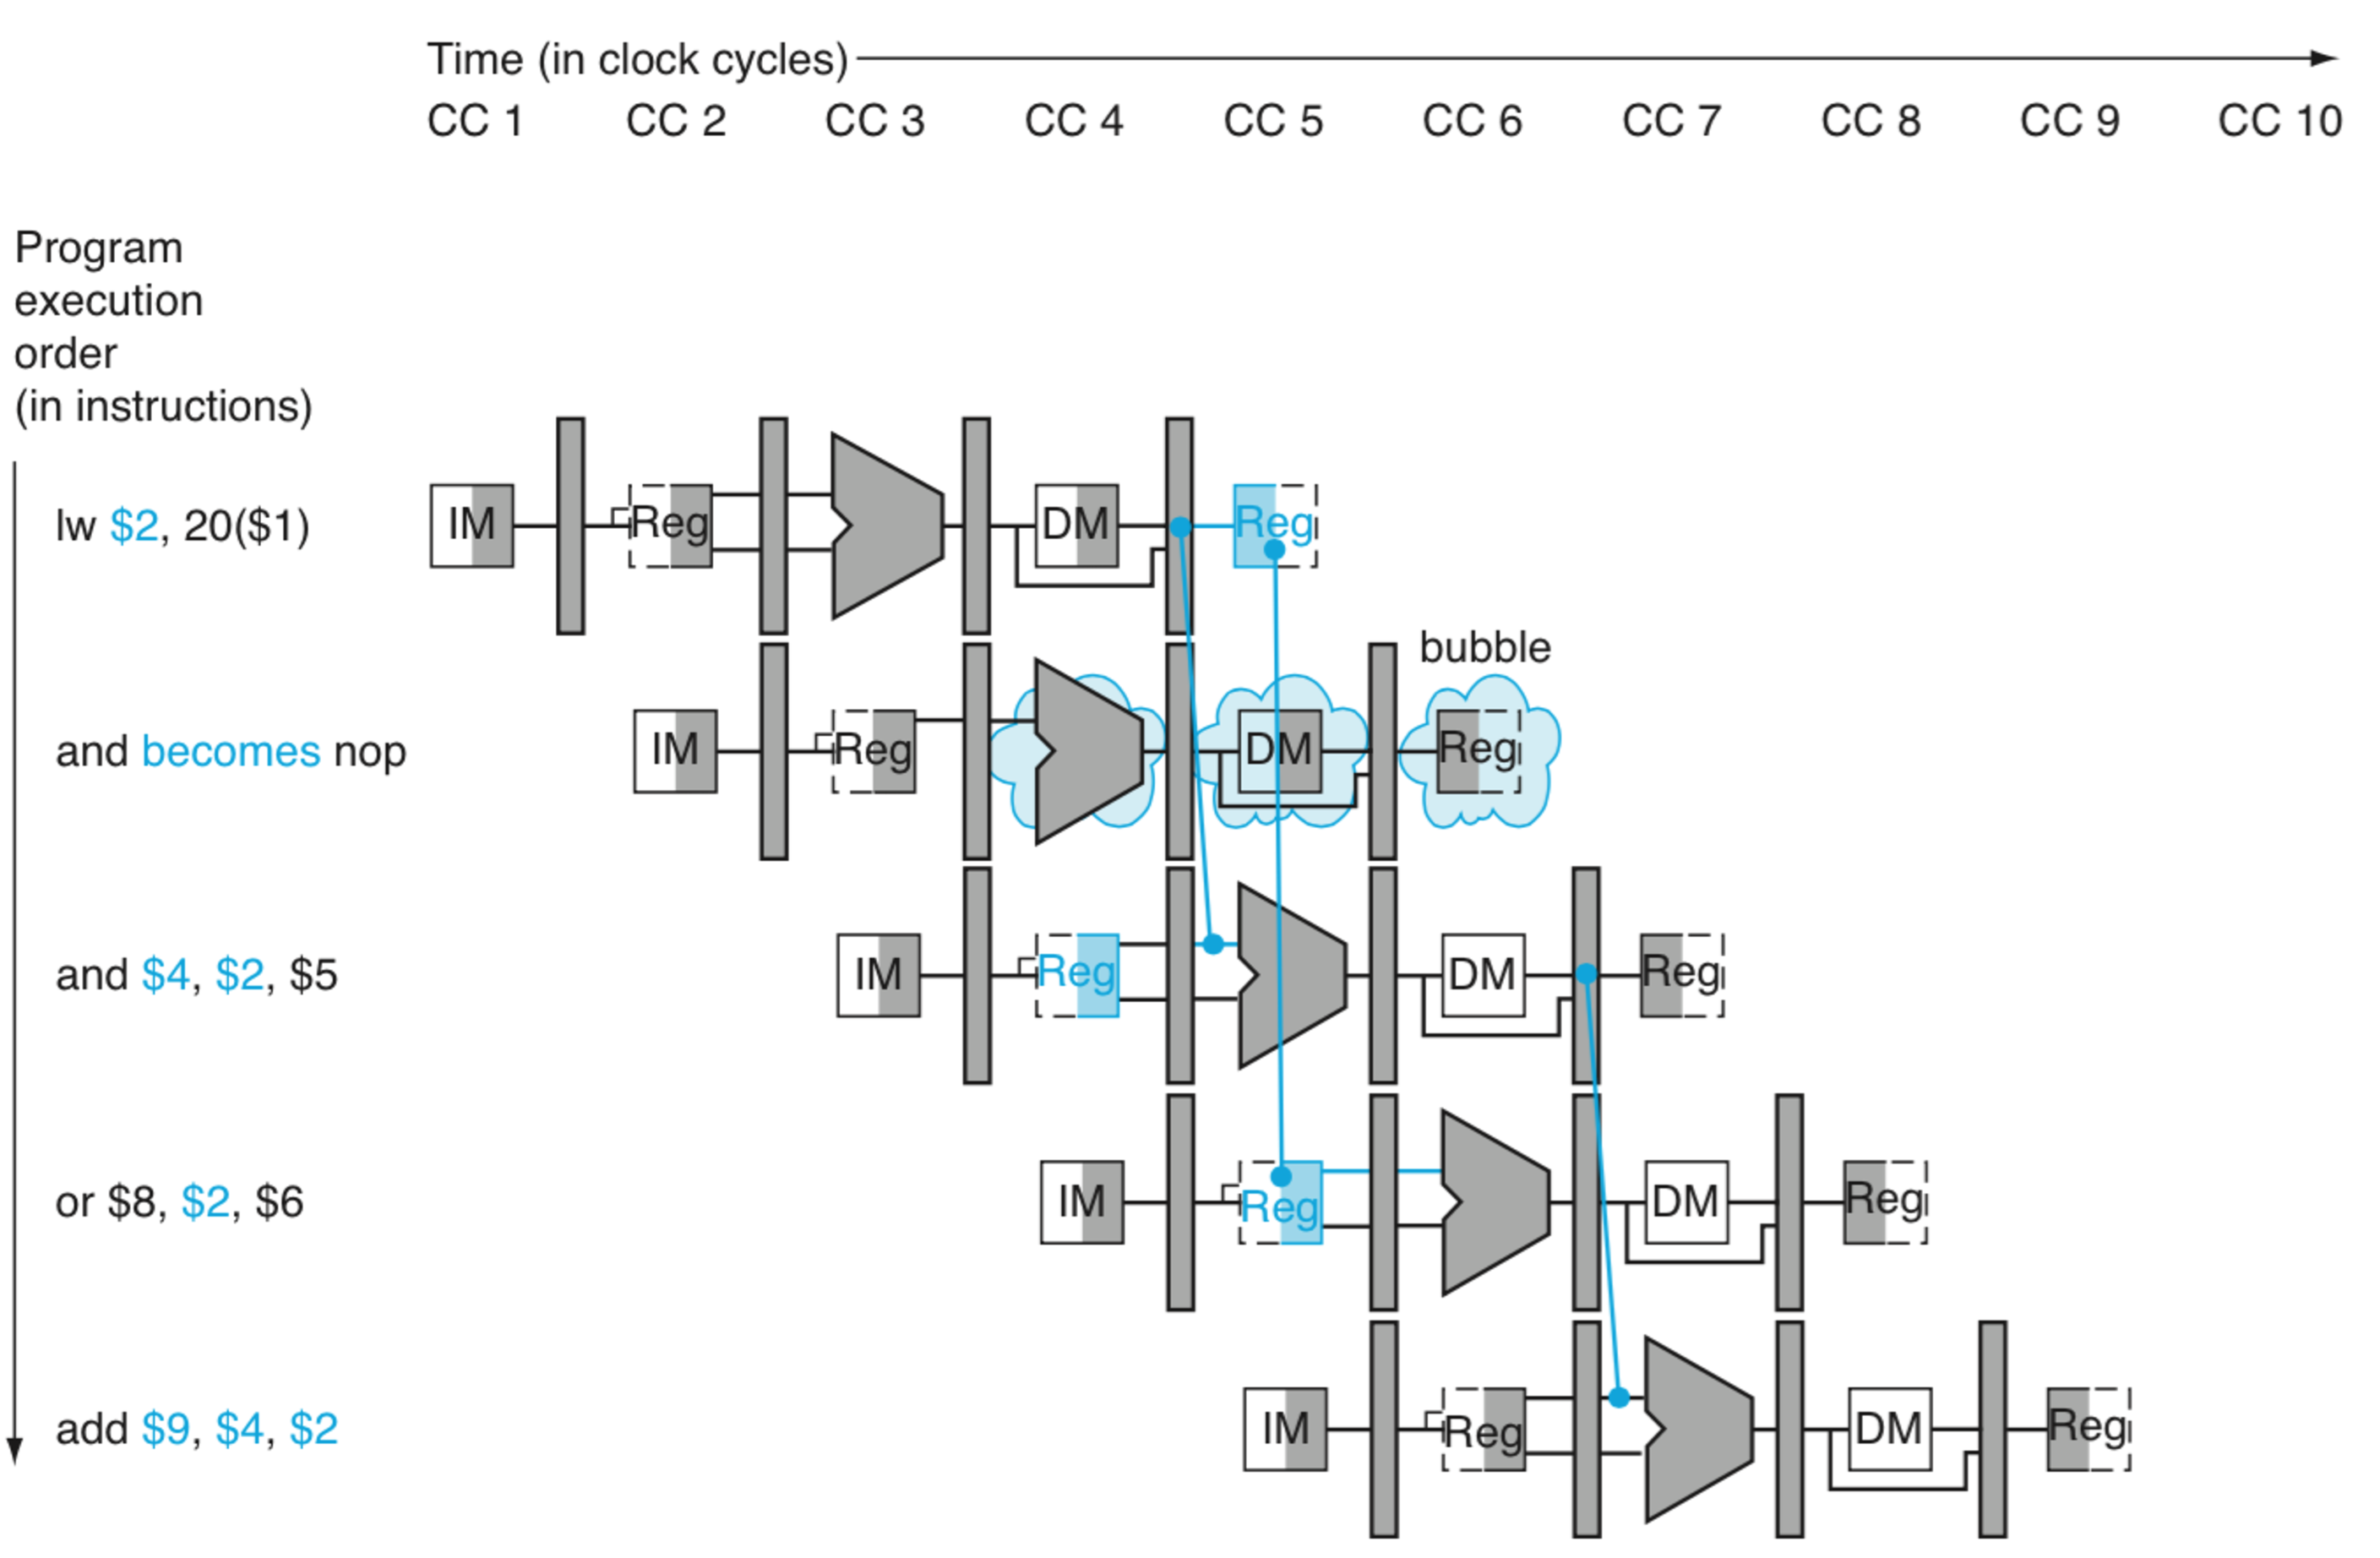
\includegraphics[width=6in]{./pics/pipelined-processor-bubbles}
\caption{An example of how bubbles/stalls can be inserted into a pipelined {\it MIPS} processor to avoid data hazards \cite{Patterson2012}.}
\label{fig:pipelinedprocessorbubbles}
\end{figure}
%    bubbles
%    Figure 6.34, Patterson2005, pp. 414
%    Figure 6.35, Patterson2005, pp. 415
%    Figure 4.58, Patterson2012, pp. 372
%    Figure 4.59, Patterson2012, pp. 374

Figure \ref{fig:pipelined-processor-data-hazards} shows an example of how some data dependencies cannot be resolved by forwarding of data values to another datapath component and these data dependencies will cause data hazards.
The register {\tt \$2} is written by the {\tt lw} instruction and is ready at the end of the fifth cycle. However, it is also required in the subsequent two instructions {\tt and} and {\tt or} in previous cycles. Hence, the data dependencies between these instructions have caused data hazards that will affect the correct functionality of the processor. To address the problem of data hazards, bubbles are used to delay the execution of instructions by flushing contents of the datapath pipeline that are associated with instructions causing these data hazards. Figure \ref{fig:pipelinedprocessorbubbles} shows how bubbles/stalls can be inserted into the datapath pipeline of a pipelined {\it MIPS} processor to avoid data hazards \cite{Patterson2012}. Bubbles (or {\tt nop} instructions) are inserted to flush contents of the ALU, memory device, and associated {\tt \$2} register in the register file. \\


Lastly, to improve the performance of pipelined processors regarding control hazards, techniques based on static branch prediction and dynamic branch prediction can be used. The former category of branch prediction techniques are carried out by compilers during compilation time, while the latter category of branch prediction techniques are carried out at run-time by the branch prediction unit in the pipelined microarchitecture \cite{Hennessy2012,Shen2005a}.










%%%%%%%%%%%%%%%%%%%%%%%%%%%%%%%%%%%%%%%%%
%	Superscalar Processor Design
%	This is written by Zhiyang Ong as a template for writing reports.

%	The MIT License (MIT)

%	Copyright (c) <2014> <Zhiyang Ong>

%	Permission is hereby granted, free of charge, to any person obtaining a copy of this software and associated documentation files (the "Software"), to deal in the Software without restriction, including without limitation the rights to use, copy, modify, merge, publish, distribute, sublicense, and/or sell copies of the Software, and to permit persons to whom the Software is furnished to do so, subject to the following conditions:

%	The above copyright notice and this permission notice shall be included in all copies or substantial portions of the Software.

%	THE SOFTWARE IS PROVIDED "AS IS", WITHOUT WARRANTY OF ANY KIND, EXPRESS OR IMPLIED, INCLUDING BUT NOT LIMITED TO THE WARRANTIES OF MERCHANTABILITY, FITNESS FOR A PARTICULAR PURPOSE AND NONINFRINGEMENT. IN NO EVENT SHALL THE AUTHORS OR COPYRIGHT HOLDERS BE LIABLE FOR ANY CLAIM, DAMAGES OR OTHER LIABILITY, WHETHER IN AN ACTION OF CONTRACT, TORT OR OTHERWISE, ARISING FROM, OUT OF OR IN CONNECTION WITH THE SOFTWARE OR THE USE OR OTHER DEALINGS IN THE SOFTWARE.

%	Email address: echo "cukj -wb- 23wU4X5M589 TROJANS cqkH wiuz2y 0f Mw Stanford" | awk '{ sub("23wU4X5M589","F.d_c_b. ") sub("Stanford","d0mA1n"); print $5, $2, $8; for (i=1; i<=1; i++) print "6\b"; print $9, $7, $6 }' | sed y/kqcbuHwM62z/gnotrzadqmC/ | tr 'q' ' ' | tr -d [:cntrl:] | tr -d 'ir' | tr y "\n"

%%%%%%%%%%%%%%%%%%%%%%%%%%%%%%%%%%%%%%%%%%%%%%


%%%%%%%%%%%%%%%%%%%%%%%%%%%%%%%%%%%%%%%%%%%
\section{Superscalar Processor Design}
\label{sec:SuperscalarProcessorDesign}


%    Hennessy2012
%    Chapter 3, 
%    
%    Hennessy2007
%    Chapter 2, 3,
%    
%    Hennessy2003
%    Chapter 3,

To improve the performance of pipelined processors, multiple instructions can be issued at the same time (i.e., superscalar instruction issue) in the pipelined microarchitecture; scalar processors can only issue one instruction per clock cycle. Therefore, superscalar processors allow the throughput of instruction execution to increase by exploiting instruction-level parallelism via instruction scheduling, loop unrolling, and branch prediction to reduce unnecessary stalls in the pipelined datapath \cite{Hennessy2012,Shen2005a}. However, the scope of literature on techniques to improve the performance of superscalar processors, including superpipelined and superscalar processors, is vast. Hence, I would only briefly mention the important concepts behind superscalar processors. \\



\begin{figure}[h]
\centering 
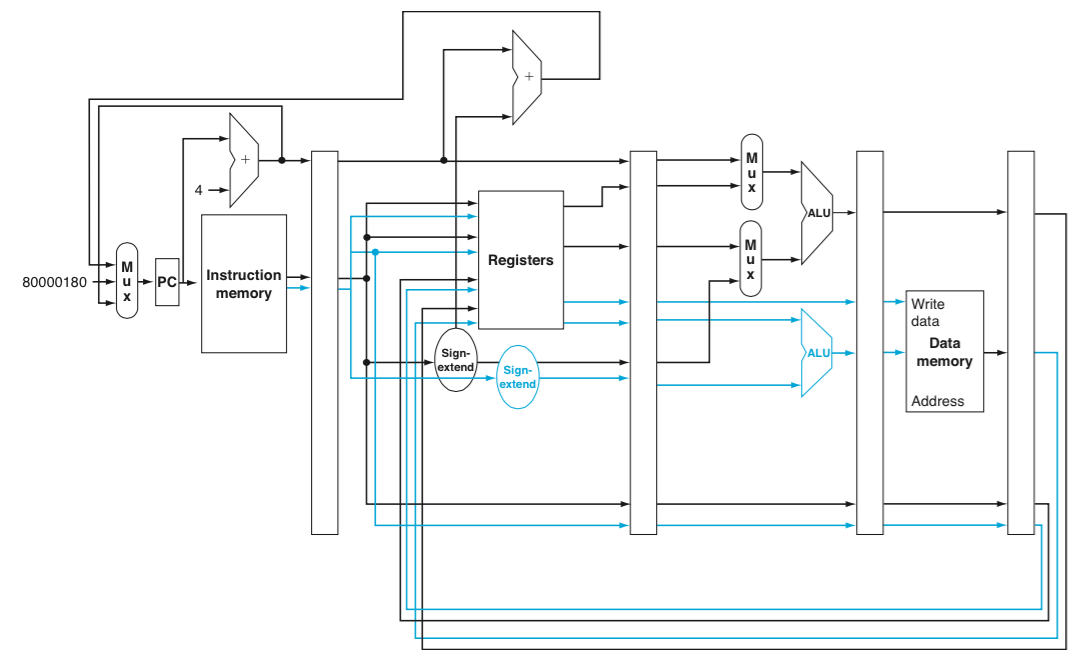
\includegraphics[width=6in]{./pics/superscalar-static-pipeline}
\caption{The static datapath pipeline of a superscalar processor \cite{Patterson2012}.}
\label{fig:superscalarstaticpipeline}
\end{figure}

\begin{figure}[h]
\centering 
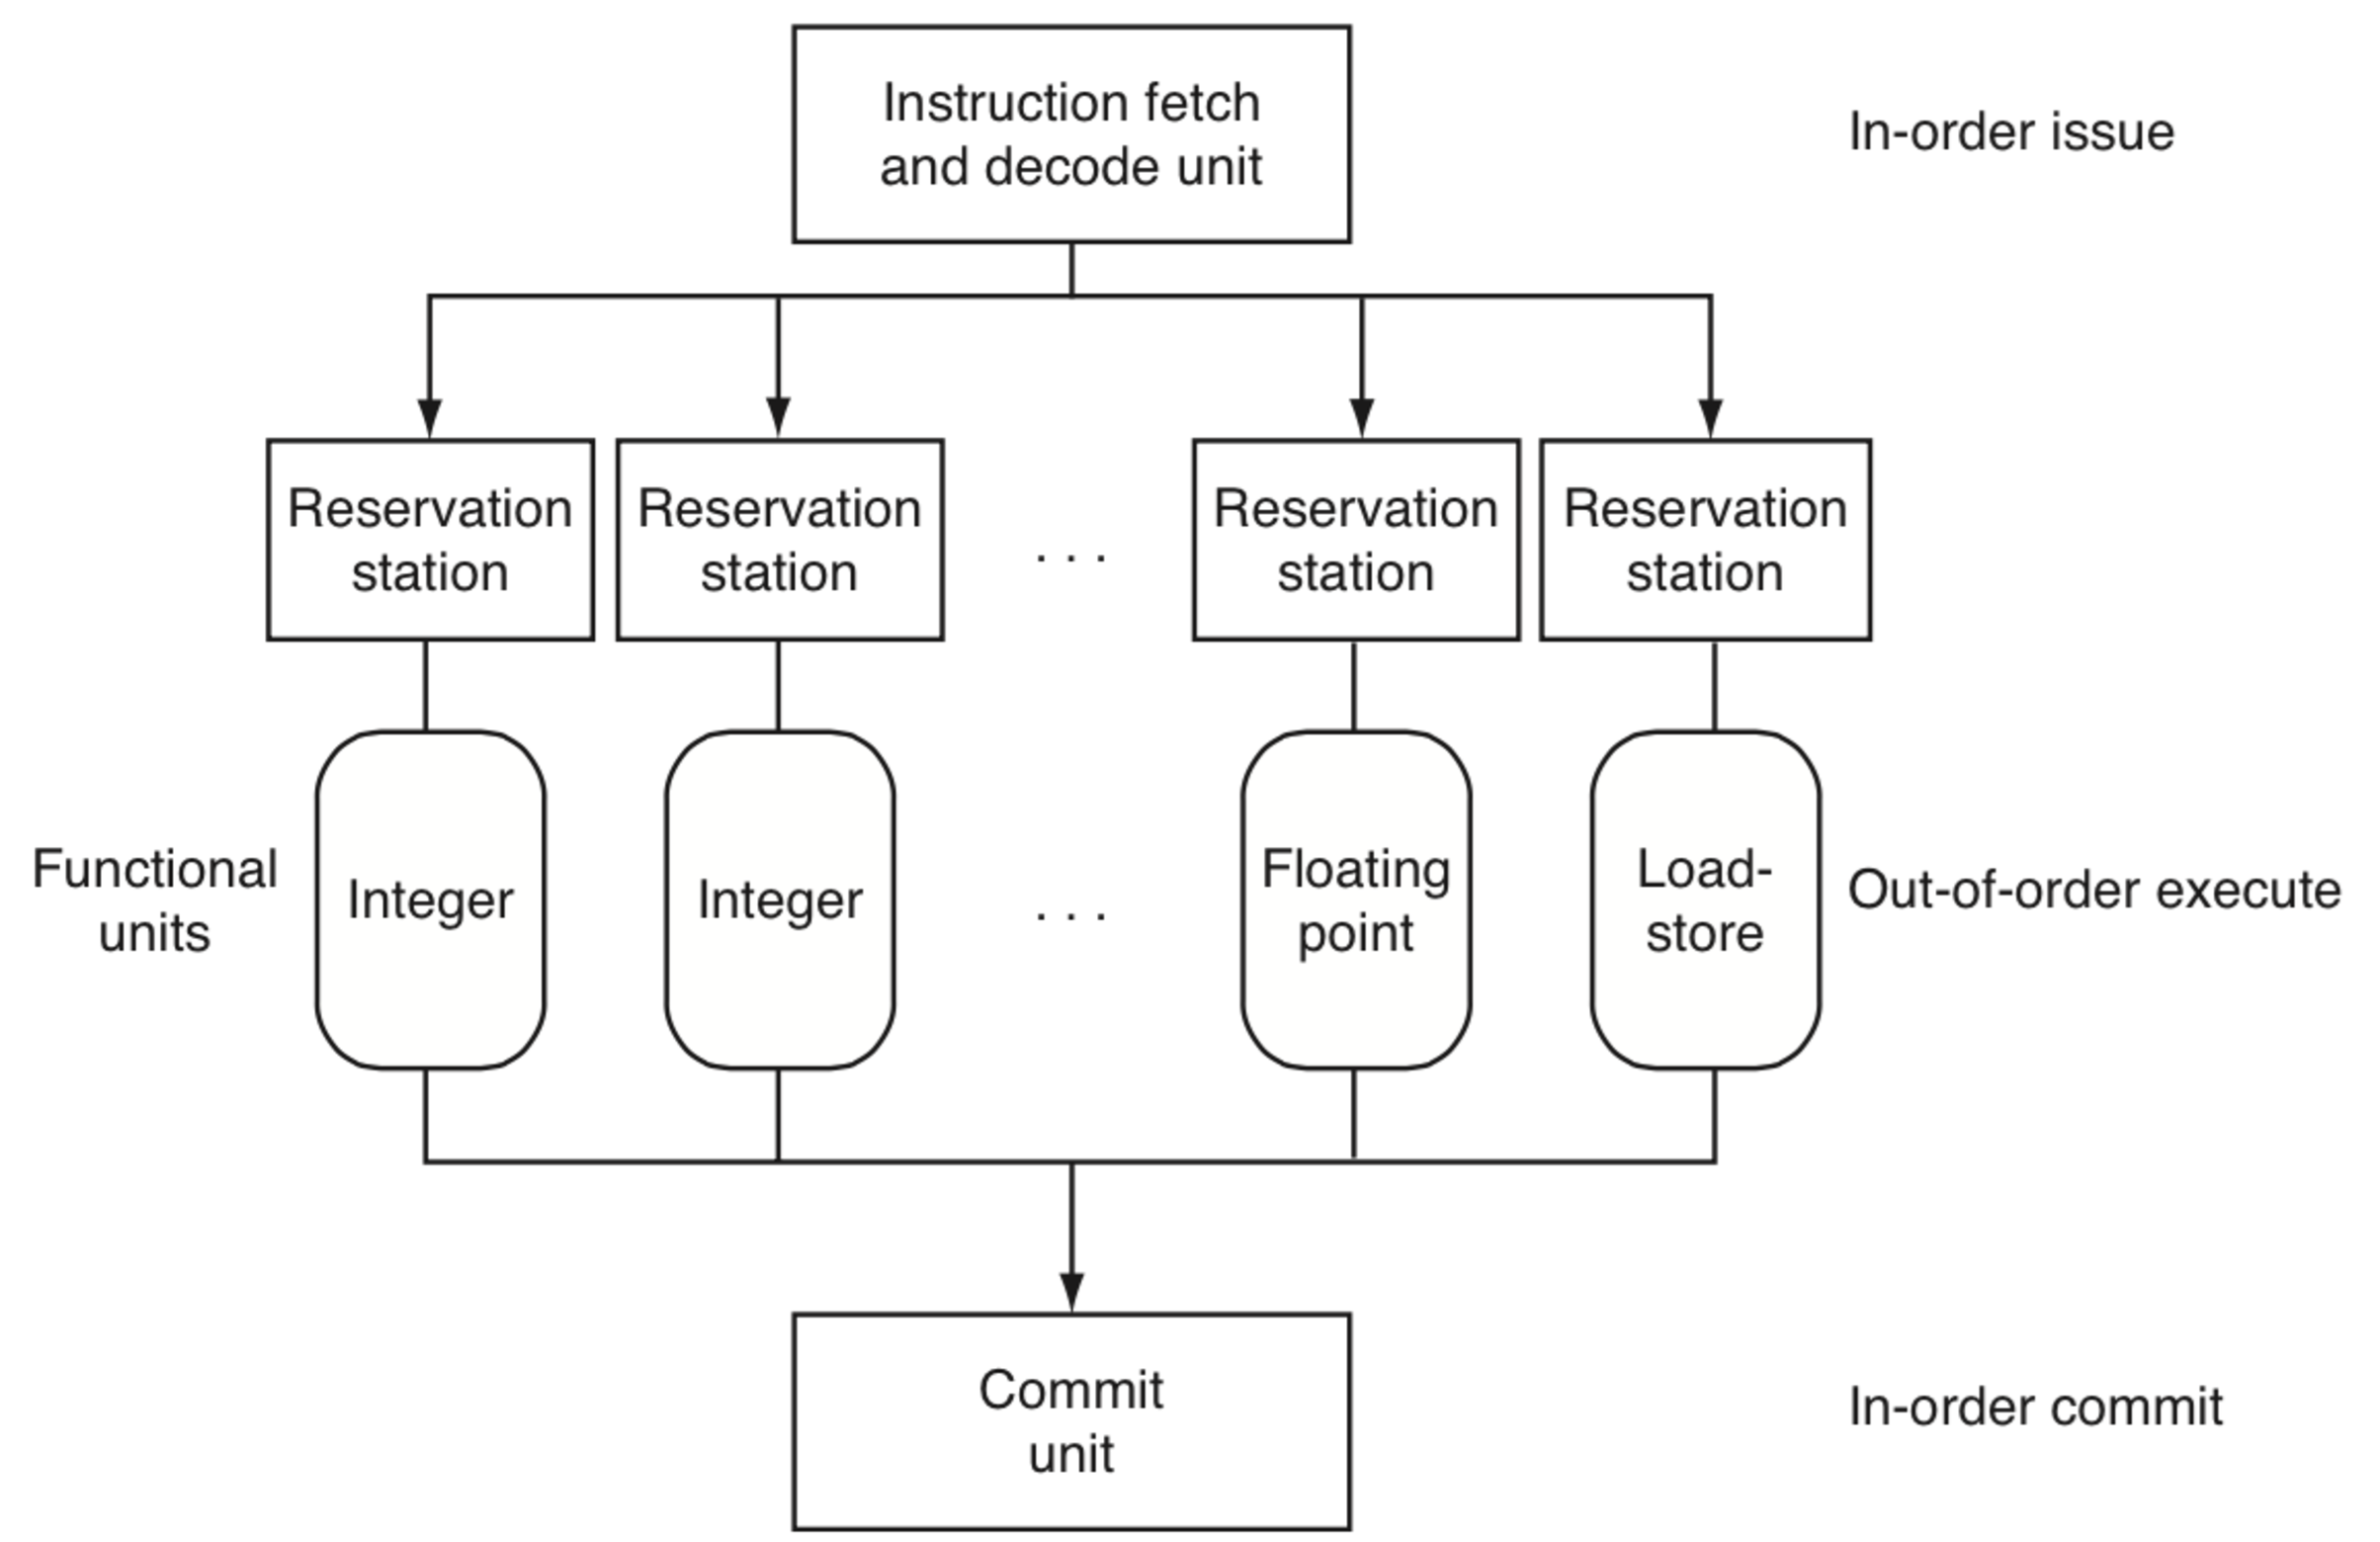
\includegraphics[width=6in]{./pics/superscalar-dynamic-pipeline}
\caption{The dynamic datapath pipeline of a superscalar processor \cite{Patterson2012}.}
\label{fig:superscalardynamicpipeline}
\end{figure}

%    static two-issue datapath 
%    Figure 6.45, Patterson2005, pp. 437
%    Figure 4.69, Patterson2012, pp. 395

%    Datapath of dynamically scheduled pipeline of $n$-issue superscalar processors
%    Figure 6.49, Patterson2005, pp. 444
%    Figure 4.72, Patterson2012, pp. 399


%    Pentium 4 datapath 
%    Figure 6.50, Patterson2005, pp. 449
%    AMD Opteron X4 microarchitecture
%    Figure 4.74, Patterson2012, pp. 405


\begin{figure}[h]
\centering 
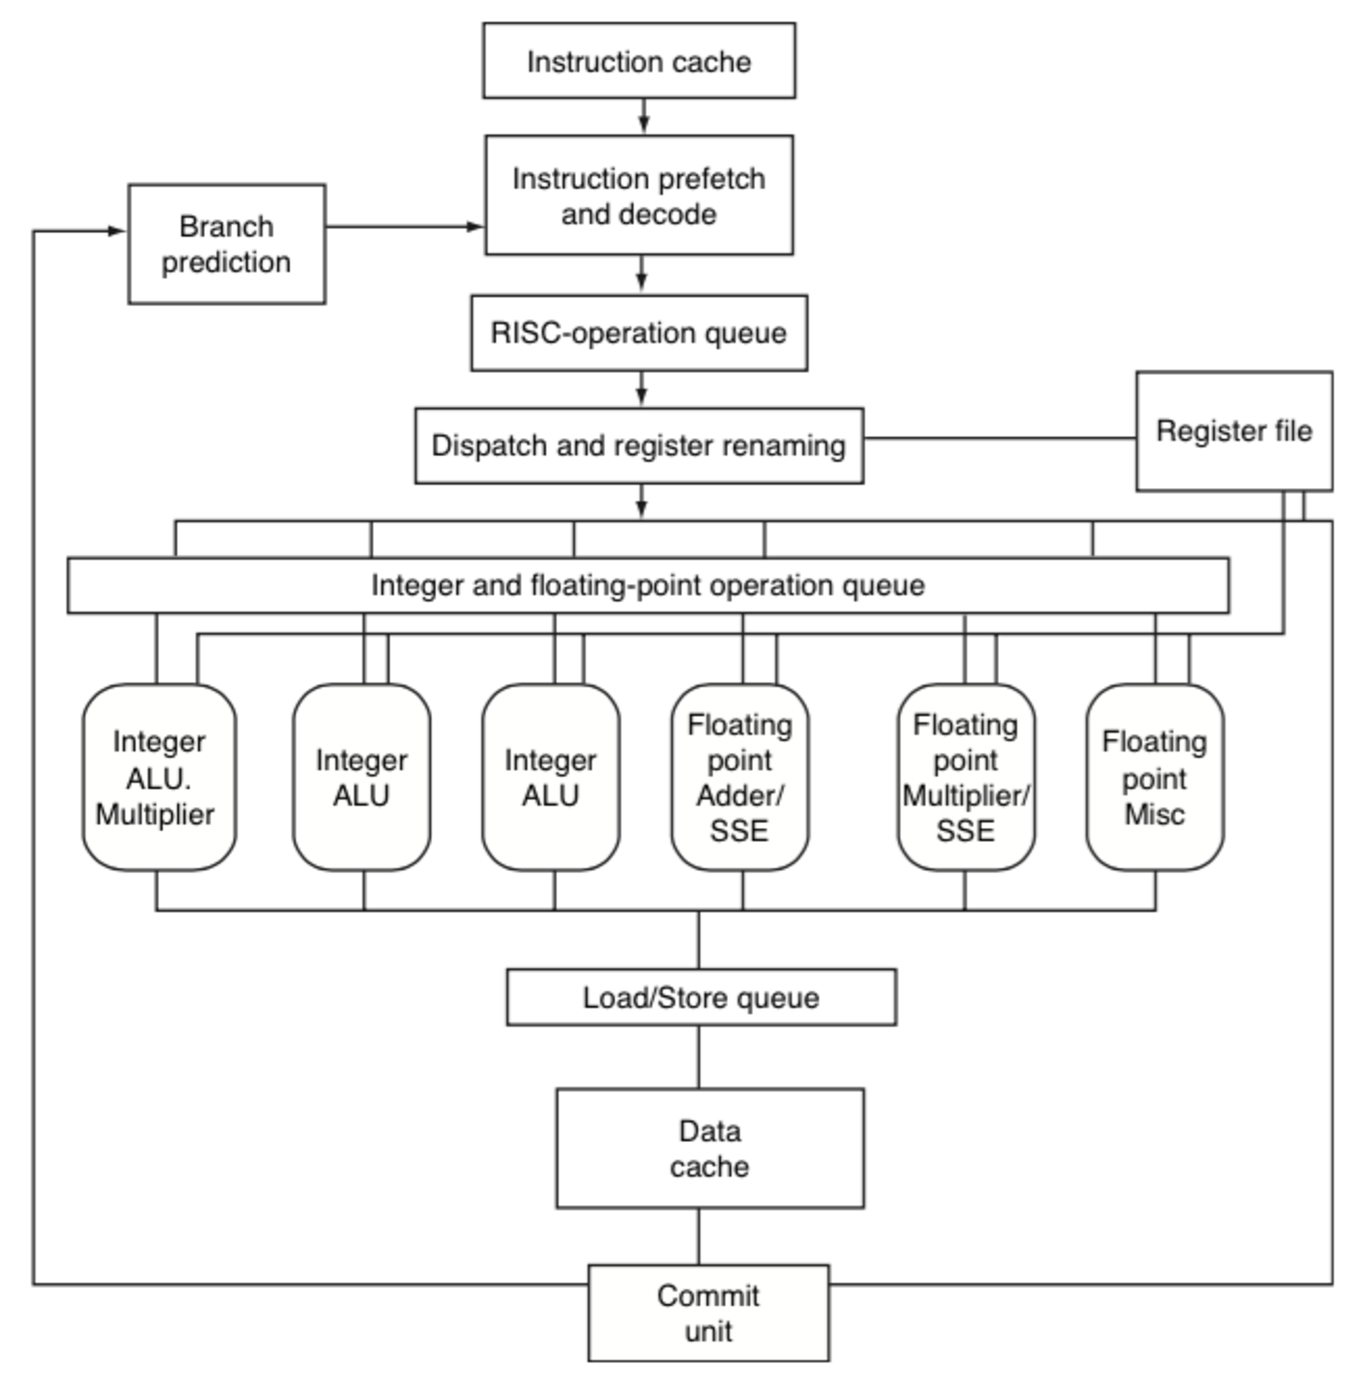
\includegraphics[width=6in]{./pics/amd-opteron-x4-uarch}
\caption{Dynamic pipelined datapath of the AMD Opteron X4 processor's microarchitecture \cite{Patterson2012}.}
\label{fig:amdopteronx4uarch}
\end{figure}

A brief description of static and dynamic pipelined, superscalar processors is provided as follows. Figure \ref{fig:superscalarstaticpipeline} shows the static datapath pipeline of a superscalar processor \cite{Patterson2012}. It issues multiple instructions per clock cycle, and has two separate datapath pipelines of functional units to support superscalar execution of instructions. In Figure \ref{fig:superscalardynamicpipeline}, a dynamic datapath pipeline of a superscalar processor is shown \cite{Patterson2012}; such superscalar processors are also known as out-of-order, superscalar processors. Instruction scheduling and loop unrolling are exploited to allow instructions to be issued in order, executed out of order (due to instruction scheduling), and completed in order so that less bubbles have to be issued in the datapath pipeline. Here, loop unrolling increases the window size of instructions that the compiler or corresponding hardware can use to carry out instruction scheduling. In order for dynamic pipelined, superscalar processors to function correctly, reservation stations (or a dispatch buffer) is placed between the front-end of the processor (for instruction fetch and decode) and the execution stage. They ensure that instructions are issued in order as they appear in the instruction stream. In addition, reorder buffers in the commit unit must be used to complete and retire the executed instructions in order. This in-order retirement of instructions guarantees the functional correctness of running computer programs on that out-of-order superscalar processor
\cite{Hennessy2012,Shen2005a}. Figure \ref{fig:amdopteronx4uarch} shows the dynamic pipelined datapath of the AMD Opteron X4 processor's microarchitecture \cite{Patterson2012}. It reflects multi-instruction issue in contemporary microarchitectures and the use of parallel functional units to support superscalar instruction issue, such as three integer ALUs in this example.




























































%%%%%%%%%%%%%%%%%%%%%%%%%%%%%%%%%%%%%%%%%
%	Conclusion
%	This is written by Zhiyang Ong as a template for writing reports.

%	The MIT License (MIT)

%	Copyright (c) <2014> <Zhiyang Ong>

%	Permission is hereby granted, free of charge, to any person obtaining a copy of this software and associated documentation files (the "Software"), to deal in the Software without restriction, including without limitation the rights to use, copy, modify, merge, publish, distribute, sublicense, and/or sell copies of the Software, and to permit persons to whom the Software is furnished to do so, subject to the following conditions:

%	The above copyright notice and this permission notice shall be included in all copies or substantial portions of the Software.

%	THE SOFTWARE IS PROVIDED "AS IS", WITHOUT WARRANTY OF ANY KIND, EXPRESS OR IMPLIED, INCLUDING BUT NOT LIMITED TO THE WARRANTIES OF MERCHANTABILITY, FITNESS FOR A PARTICULAR PURPOSE AND NONINFRINGEMENT. IN NO EVENT SHALL THE AUTHORS OR COPYRIGHT HOLDERS BE LIABLE FOR ANY CLAIM, DAMAGES OR OTHER LIABILITY, WHETHER IN AN ACTION OF CONTRACT, TORT OR OTHERWISE, ARISING FROM, OUT OF OR IN CONNECTION WITH THE SOFTWARE OR THE USE OR OTHER DEALINGS IN THE SOFTWARE.

%	Email address: echo "cukj -wb- 23wU4X5M589 TROJANS cqkH wiuz2y 0f Mw Stanford" | awk '{ sub("23wU4X5M589","F.d_c_b. ") sub("Stanford","d0mA1n"); print $5, $2, $8; for (i=1; i<=1; i++) print "6\b"; print $9, $7, $6 }' | sed y/kqcbuHwM62z/gnotrzadqmC/ | tr 'q' ' ' | tr -d [:cntrl:] | tr -d 'ir' | tr y "\n"

%%%%%%%%%%%%%%%%%%%%%%%%%%%%%%%%%%%%%%%%%%%%%%


%%%%%%%%%%%%%%%%%%%%%%%%%%%%%%%%%%%%%%%%%%%
\section{Conclusion}
\label{sec:Conclusion}

%By examining the different microarchitectural implementations of the {\it MIPS} ISA, we can conclude that the ISA determines various aspects of a microarchitecture for that ISA. For example, the microarchitecture for a RISC processor would have a simpler control unit/path than the microarchitecture for a CISC processor. Also, we can observe that the microarchitecture design of a processor affects the performance of the computer system, since the clock rate (CCT) and the CPI for the processor is determined by its microarchitecture \cite{Patterson2005}. \\
By examining the different microarchitectural implementations of the {\it MIPS} ISA, we can conclude that the ISA determines various aspects of a microarchitecture for that ISA. For example, the microarchitecture for a multi-cycle processor (see Figure \ref{fig:multicycleprocessor}) would have a simpler control unit/path than the microarchitecture for a pipelined processor (see Figure \ref{fig:pipelinedprocessor}). Also, we can observe that the microarchitecture design of a processor affects the performance of the computer system, since the clock rate (CCT) and the CPI for the processor is determined by its microarchitecture \cite{Patterson2005}. \\

Furthermore, there is a trade-off between hardware complexity (and hence, design effort and power consumption) and performance for the three scalar processor architectures (single-cycle, multi-cycle, and pipelined processors) that are considered. Microarchitectures that have better performance have more hardware complexity, in terms of the datapath and the control path. For example, the aforementioned multi-cycle processor performs better than the single-cycle processor at the cost of more hardware complexity (in the datapath and the control path). Also, the pipelined processor trades off more hardware complexity than the multi-cycle processor for better performance. However, as we add move to superscalar and superpipelined microarchitectures \cite{Jouppi1989}, we have to consider a more nuanced trade-off between hardware complexity for the issue logic, instructions per cycle (IPC) (see Equation \ref{eqn:ipcandcpi} for its definition), and computer performance \cite{Hrishikesh2002,Palacharla1998}. Comparing a heavily pipelined processor architecture to a not-so-heavily pipelined processor, the former may have worse performance than the latter, since the former would have a greater proportion of pipeline overhead per clock cycle. It means that the heavily pipelined processor wastes more computational resources for inefficient work than the not-so-heavily pipelined processor. Similarly, when comparing a superscalar processor with a wider instruction issue width to another superscalar processor of narrower instruction issue width, the former would have greater inefficiency than the latter. This is because the former would have greater hardware complexity (in terms of logic/circuit and wiring complexities) than the latter. Also, after issuing instructions in order, the former would spend more computational resources than the latter in trying to execute instructions out of order and retiring them in order \cite{Shen2005a,Hennessy2012}. \\
%An heavily pipelined processor architecture may have worse performance than a less pipelined processor, since the heavily pipelined processor architecture would have a greater proportion of pipeline overhead per clock cycle for inefficient work in comparison to the less pipelined processor. 
%Similarly, the hardware complexity (in terms of logic/circuit and wiring complexities) for a superscalar processor that has a wider instruction issue width would have greater inefficiency than superscalar processors of narrower instruction issue width in spending computational resources trying to execute instructions out of order and 

%	Figure 6.52 and 6.53, Patterson2005, pp. 453

\begin{figure}[h]
\centering 
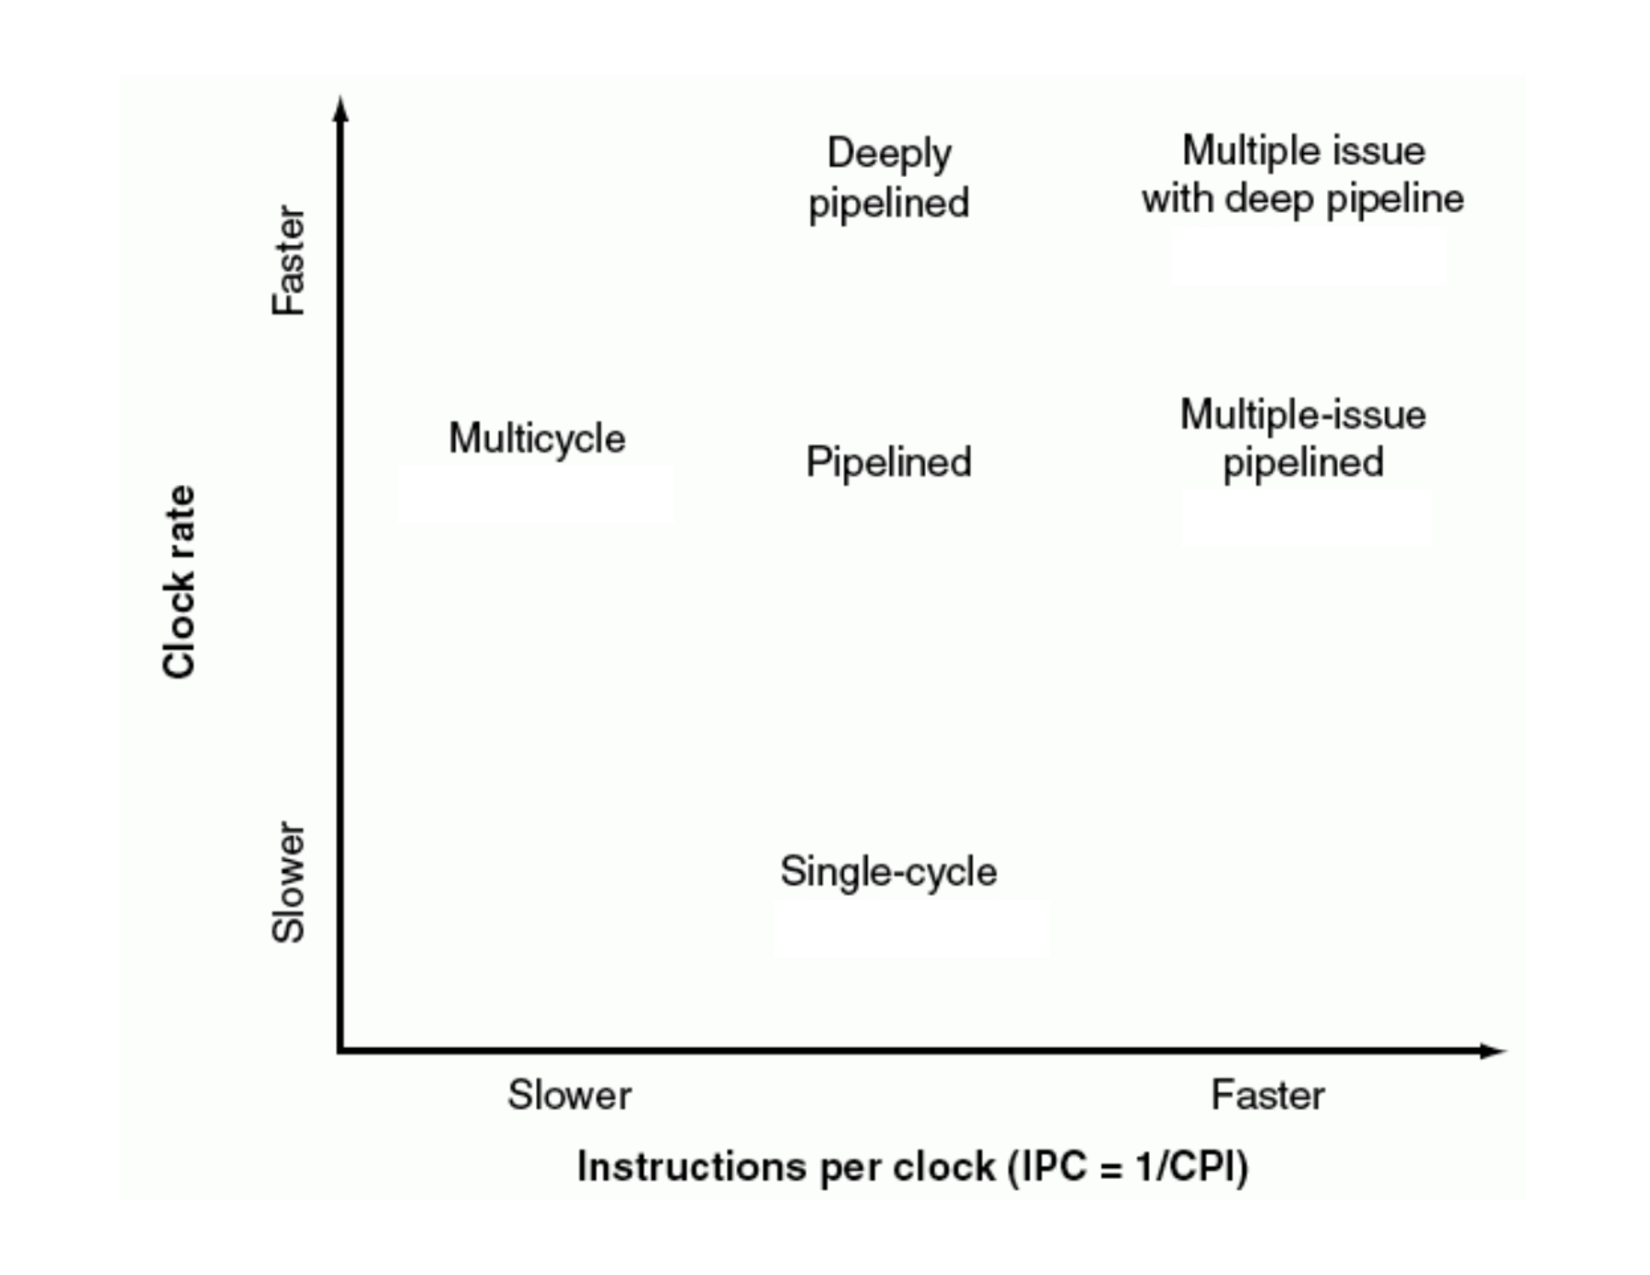
\includegraphics[width=6in]{./pics/frequency-vs-ipc}
\caption{Plot of clock frequency versus instructions per clock cycle (IPC) \cite{Patterson2005}. $IPC = \frac{1}{CPI}$ (see Equation \ref{eqn:ipcandcpi}), where {\it CPI} refers to clock cycles per instruction (see Section \ref{sec:IntroProcessorArchitecture}). From the ``iron law'' in Equation \ref{eqn:ironlaw}, the clock rate (CCT) and IPC (or $\frac{1}{CPI}$) affects the performance of the processor. Hence, as we move from design solutions in the bottom-left corner towards those in the top-right corner, we can find design solutions that have better computer performance.}
\label{fig:frequencyvsipc}
\end{figure}

%In Figure \ref{fig:frequencyvsipc}, a plot of clock frequency (i.e., clock rate) versus instructions per clock cycle (IPC) is shown \cite[Figure 6.52, pp. 453]{Patterson2005}. {\it IPC} is determined as follows \cite{Shen2005a}:
In Figure \ref{fig:frequencyvsipc}, a plot of clock frequency (i.e., clock rate) versus instructions per clock cycle (IPC) is shown \cite{Patterson2005}. {\it IPC} is determined as follows \cite{Shen2005a}:
\begin{equation}
\label{eqn:ipcandcpi}
IPC = \frac{1}{CPI},
\end{equation}

where {\it CPI} refers to clock cycles per instruction (see Equation \ref{eqn:ironlaw}). The performance of a processor architecture design improves as design choices are enumerated from the bottom-left corner of Figure \ref{fig:frequencyvsipc} towards its top-right corner. Data and control dependences of instructions in any given computer program limit how much instruction-level parallelism (ILP) can be exploited with pipelining and multiple instruction issue (i.e., superscalar processor design) for out-of-order execution. Therefore, in modern superscalar processor designs, instruction scheduling, dynamic branch prediction, and hardware speculation are used to improve processor performance \cite{Patterson2005,Shen2005a,Hennessy2012}. \\

A plot of the amount of hardware resource sharing versus instruction latency is shown in Figure \ref{fig:amountofhwsharingvsinstructionlatency}. Like in Figure \ref{fig:frequencyvsipc}, the performance of a processor architecture design improves as design choices are enumerated from the bottom-left corner towards the top-right corner. As aforementioned, pipelining and the width of instruction issue cannot be increased indefinitely without incurring performance penalty; this is the ``ILP wall''. Recent history indicates that the ``memory wall'' and the ``power wall'' have become bottlenecks in microarchitecture design; the ``memory wall'' refers to the diverging rates of performance improvement between the processor and physical memory (i.e., main memory), and the ``power wall'' refers to the increasing power consumption of advanced processor designs from the late 1980s till the early 2000s. Hence, the processor design industry has shifted towards designing chip multiprocessors to improve computer performance \cite{Hennessy2012,Wulf1995}. \\

\begin{figure}[h]
\centering 
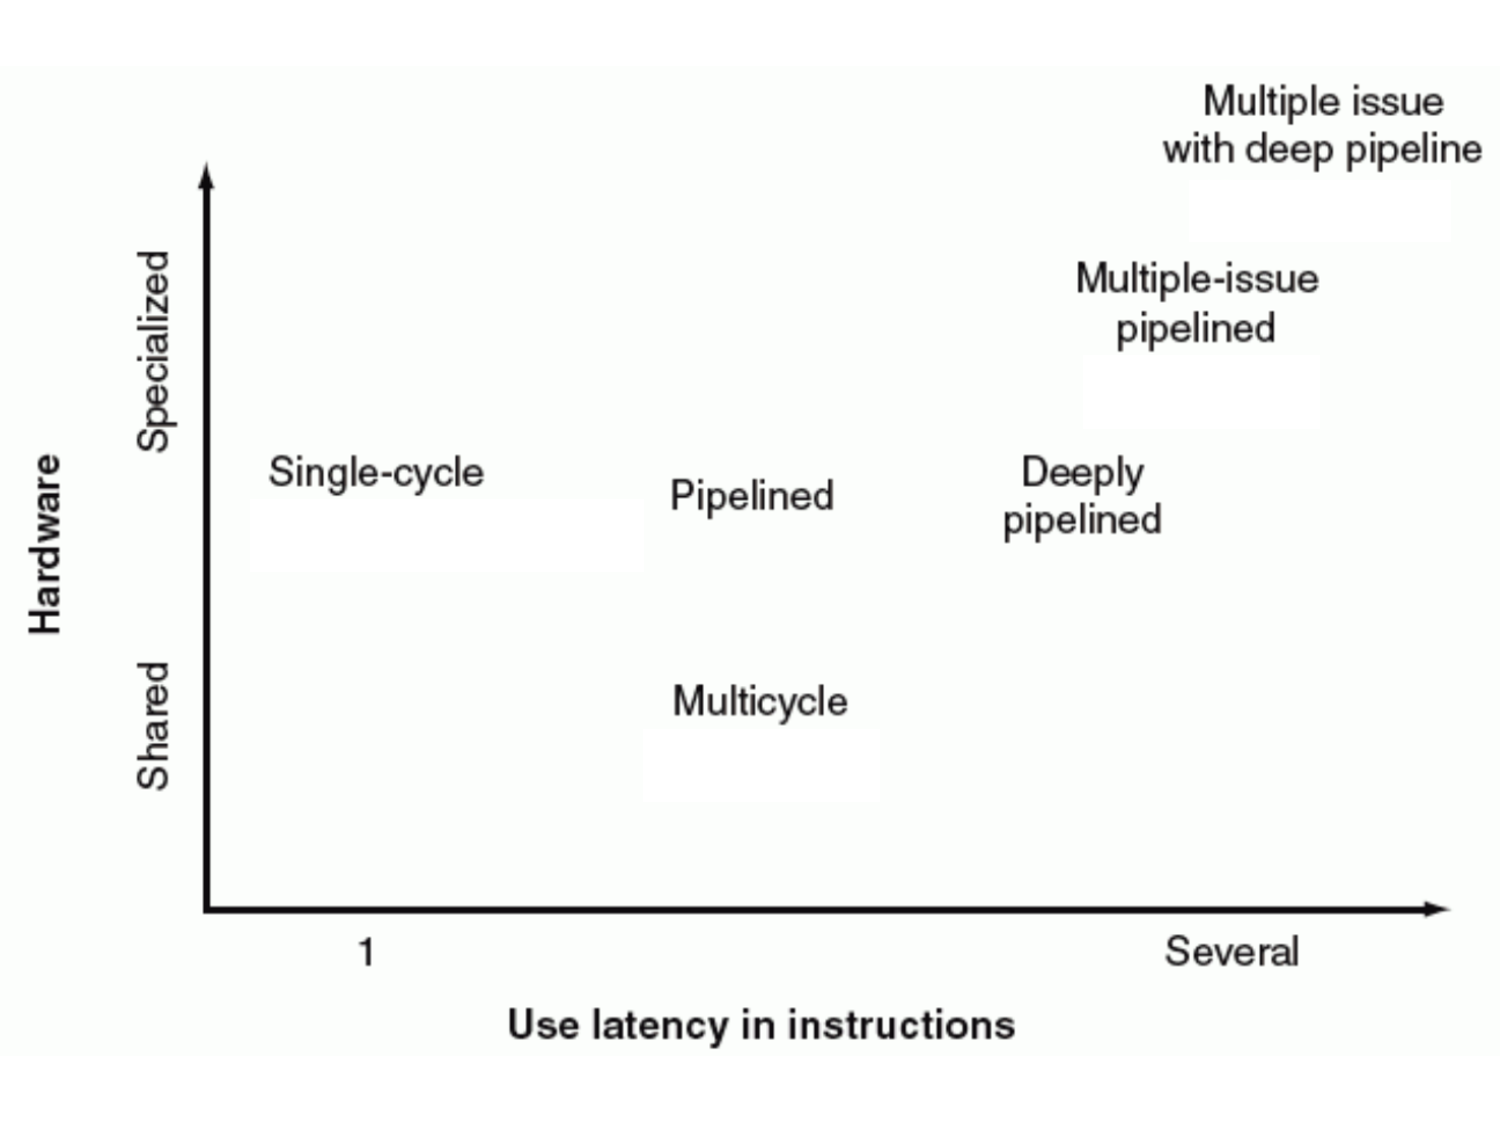
\includegraphics[width=6in]{./pics/amount-of-hw-sharing-vs-instruction-latency}
\caption{Plot of the amount of hardware resource sharing versus use latency in instructions \cite{Patterson2005}. The $y$-axis indicates the amount of specialized hardware that is used to execute instructions in a computer program, while the $x$-axis represents how easy it is to utilize all pipeline stages in a pipelined processor. As we move from design solutions in the bottom-left corner towards those in the top-right corner, we can find design solutions that have better computer performance.}
\label{fig:amountofhwsharingvsinstructionlatency}
\end{figure}



Hence, wisdom and insight about the applications that a processor would run can be used while considering trade-offs between hardware complexity (as well as design effort and power consumption) with performance. However, performance speedup need not come with only microarchitectural improvements. Performance speedup can also come from designing computer architectures for other computing paradigms (such as re-revisiting dataflow processor architectures \cite{Dennis1974}). It can also come using alternative computer system design paradigms, such as application-specific instruction set processors \cite{Gries2005,Karuri2011,Schliebusch2007}, neuromorphic processors \cite{Benjamin2014,Misra2010,Merolla2011,Seo2011,Kim2014,Kim2013a} and other cognitive computers, and general-purpose graphics processing units \cite{Altman2011,Kim2012,Kirk2010}. \\

Lastly, to paraphrase Prof. Roberto Sebastiani \cite{Sebastiani2007a}, neither the problem of designing an efficient processor architecture, nor that of acquiring a comprehensive background of microarchitecture is easy. The challenge of designing high-performance, energy-efficient processor architectures is not just a daunting engineering task, but also an art in itself.




























%%%%%%%%%%%%%%%%%%%%%%%%%%%%%%%%%%%%%%%%%%%
\section*{Acknowledgements}
\label{sec:Acknowledgements}
\addcontentsline{toc}{section}{Acknowledgements}

I would like to thank Prof. Richard McGuire and my classmates of my ``Scientific Writing'' class for helping me improve my technical writing skills. In addition, I would like to thank Ms. Kadie Henderson and Ms. Laura from the University Writing Center at Texas A\&M University for reviewing my work and for helping me to find mistakes and errors in my report. 

%%%%%%%%%%%%%%%%%%%%%%%%%%%%%%%%%%%%%%%%%
%	Bibliography
%\input{./others/bibliography}





%%%%%%%%%%%%%%%%%%%%%%%%%%%%%%%%%%%%%%%%%%%%%
%%%%%%%%%%%%%%%%%%%%%%%%%%%%%%%%%%%%%%%%%%%%%
%
%	End of document
%
%	Inserting references
%
%%%%%%%%%%%%%%%%%%%%%%%%%%%%%%%%%%%%%%%%%%%%%
%%%%%%%%%%%%%%%%%%%%%%%%%%%%%%%%%%%%%%%%%%%%%
%	Beginning of BACK MATTER: bibliography, indexes and colophon
%\backmatter
\appendix

{\linespread{1}
\bibliographystyle{plain}
%\bibliography{./references/references}
\bibliography{/data/research/antipastobibtex/references}
\addcontentsline{toc}{section}{Bibliography}
}
\end{document}